\documentclass{article}
\usepackage{longtable}
\usepackage{xcolor}
\usepackage{enumitem}
\usepackage{geometry}
\usepackage{float}
\usepackage{url}
\usepackage{graphicx}
\usepackage{amsmath}
\usepackage{listings}
\usepackage{microtype}
\usepackage{hyperref}
\usepackage{adjustbox}

\newcommand\ytl[2]{
    \parbox[b]{12em}{\hfill{\color{cyan}\bfseries\sffamily #1}~$\cdots\cdots$~}\makebox[0pt][c]{$\bullet$}\vrule\quad
    \parbox[c]{10cm}{\vspace{6pt}\color[RGB]{20, 20, 90}\raggedright\sffamily #2\par}
    \\[-2pt]
}

\title{Creating Software for Value at Risk}
\author{Benjamin Shearlock}

\begin{document}
\raggedright

\begin{titlepage}
  \begin{center}
    \vspace*{1cm}
    {\LARGE \textbf{Creating Software for Value at Risk} \par} 
    \vspace{1.5cm}
    {\Large \textit{Final Report} \par}
    \vspace{0.5cm}
    {\Large BSc Final Year Project \\ 2024 \par}
    \vspace{2cm}
    {\large \textbf{Author} \par}
    {\large Benjamin Shearlock \par}
    \vspace{2cm}
    {\large \textbf{Supervisor} \par}
    {\large Dr. Volodya Vovk \par}
    \vfill
    {\large Department of Computer Science \par}
    {\large Royal Holloway, University of London \par}
  \end{center}
\end{titlepage}

\setlength{\parindent}{0pt}

\section*{Declaration}
I have read and understood the Universities regulations on plagiarism and I hereby declare that all work submitted in this project is my own, except where explicitly stated otherwise, such as the references that have been cited. \\

\begin{itemize}
  \item Word Count:
  \item Name: Benjamin Charles Shearlock
  \item Submission Date: 12/04/2024
  \item Youtube Video showcasing Final Deliverable Program: \url{}
  \item All other programs included within my PROJECT Git repository are simple python programs that can just be ran normally, these mainly being found within the ``Command Line VaR Programs'' folder. The GUI program has been compiled into a .exe file within the main directory, called “Initial Design Test.exe”, it will open up a terminal when ran but please ignore it, it should work perfectly otherwise. The code for it is within the ``Kivy'' folder, that has other kivy tests inside it as well. It is all in the branch ``Master'', as I was having issues with my ``Main'' branch.
  \item ADD A SECTION HERE ON HOW TO RUN THE SOFTWARE, ALSO EDIT AND CHANGE THE ABOVE ETC.

  % \item Signature: \includegraphics[scale=0.1]{Signature.png}
\end{itemize}

\newpage

\tableofcontents

\newpage

\section{Abstract}
In the realm of financial risk management, understanding and evaluating the level of risk associated with any investment or portfolio is of extremely high importance. Perhaps the most universally regarded metric used for this purpose is Value at Risk (VaR). VaR provides a quantitative estimate of the potential losses that a portfolio may incur over a certain period of time (specified time horizon) at a given confidence level. \\\vspace{0.3cm}

Original widespread use of VaR came about in the early 1990s, the concept first being introduced by J.P. Morgan in 1994, since it helped provide an estimate of the maximum loss an investor is willing to accept for any given investment. Its historical roots can be traced back to the financial industry's increasing need for a standardized and comprehensive measure of risk following the 1987 stock market crash, so they sought a comprehensive way to assess risk in complex portfolios [\ref{ref3}]. \\

Mathematically, VaR is expressed as follows:
\begin{equation}
VaR(N, X) = -\text{Percentile}(L, 1 - X)
\end{equation}
Where:
\begin{align*}
N & : \text{Time horizon (in days)} \\
X & : \text{Confidence level (in percentage)} \\
L & : \text{Loss distribution over } N \text{ days}
\end{align*}

This formula captures the loss at the \((100-X)\)th percentile of the loss distribution over the specified time horizon [\ref{ref6}]. \\\vspace{0.3cm}

VaR can be mathematically computed through various methods, each with its own strengths and limitations. The most common approaches include the historical simulation method, parametric method, model building method and Monte Carlo simulation [\ref{ref1}], to list a few. For historical simulation, past data is used to estimate future risk by examining the historical returns of an asset or portfolio, while model building employs mathematical models to predict portfolio performance. The choice of algorithm depends on data availability, computational resources, and specific requirements.\\\vspace{0.3cm}

To implement VaR calculations, various pieces of software are essential. In this project, I will be utilising Visual Studio Code (VSCode) as the integrated development environment (IDE) and Python for its rich ecosystem of libraries. Python libraries like NumPy, Matplotlib, and Kivy will be invaluable for data manipulation, visualisation, and user interface design [\ref{ref9}].\\\vspace{0.3cm}

My inaugural proof of concept program will be created to visually demonstrate VaR calculations for  two initial methods, these being historical simulation and model building techniques to estimate VaR for a sample portfolio. Historical simulation would involve collecting historical data and computing VaR based on past performance (can involve acquiring stock data through an API), while model building would use a predefined model to forecast future losses. Visualisation tools like Matplotlib can help in presenting the results graphically, enabling me to generate informative charts and graphs. NumPy will facilitate data manipulation and efficient mathematical operations [\ref{ref10}]. Additionally, Kivy, a Python framework for developing multi-touch applications, will be used to create the interfaces for the visual representation of VaR, as well as giving it the option to possibly be viewed on other devices.\\\vspace{0.3cm}

Later on into the project, if there is enough time, I think it may be worth exploring some more advanced topics like the variance-covariance of returns, specifically employing GARCH (Generalized Autoregressive Conditional Heteroscedasticity) models. GARCH models provide a more nuanced understanding of volatility and can enhance the accuracy of VaR estimates [\ref{ref6}].\\\vspace{0.3cm}

The objective of my project is to gain a deeper understanding of VaR, develop a functional program to calculate and visualise it, and potentially extend the research to incorporate more advanced risk management techniques if possible. This project is a stepping stone towards a deeper understanding of the risk side of finances and will contribute to enhancing the knowledge and skills necessary for effective financial decision-making, since this is not a topic that I have delved much into before, but I have aways been very interested in learning more about it. This gives me a fantastic opportunity to learn about the financial sector, as well as create something that is applicable and useful to real life. \\


% \section{Specification}

\newpage
\section{Chapter 1 - Introduction}

\subsection{What is VaR?}

Value at Risk (VaR) is a statistical value used to quantify the level of financial risk within a portfolio of stocks/derivatives over a specified time horizon. It estimates the maximum potential loss that an investment portfolio could incur with a given probability, known as the confidence level, under normal market conditions. The VaR metric is typically expressed in monetary terms and is often used to assess the risk of a portfolio of financial instruments. From a banks perspective, they would say:
\begin{quote}
  ``With \textbf{X\% confidence (1-X\% Risk Level)}, we expect to not lose more than \textbf{V} over the next \textbf{N day(s)} on our entire \textbf{portfolio} of derivatives, worth \textbf{Z}'' - [\ref{ref4}]

\end{quote}

Where:
\begin{align*}
  \textbf{X} & : \text{Confidence Level} \\
  \textbf{V} & : \text{Value at Risk} \\
  \textbf{N} & : \text{Time Horizon} \\
  \textbf{Z} & : \text{Portfolio Value}
\end{align*}

This is incredibly useful as it allows for a simple and easy to understand metric to be used to assess the risk of a portfolio, which is extremely important in the financial sector, taking all the underlying complexities of any form of portfolio and being able to conform its financial risk into a single, universally used, number. \\\vspace{0.3cm}

To include actual numbers, to easier explain how it would look, a bank would say:
\begin{quote}
  ``With \textbf{95\%} confidence (\textbf{5\%} Risk Level), we expect to not lose more than \textbf{£3,000,000} over the next \textbf{1 day} on our entire portfolio of derivatives, worth \textbf{£100,000,000}''
\end{quote}

This is essential to help financial institutions understand the level of risk associated with their portfolios, as well as being able to compare the risk of different portfolios, which is why it is such a widely used metric in the financial sector, limiting the level of risk that a person/organisation is exposed to.\\\vspace{0.3cm}

The concept of VaR has its roots in the late 20th century, gaining prominence in the finance industry during the 1990s. It emerged from the need for more sophisticated risk management tools in the wake of financial market liberalisation and the increasing complexity of financial instruments. The widespread adoption of VaR was catalysed by the 1998 financial crisis, where it played a significant role in risk assessment and regulatory frameworks.\\\vspace{0.3cm}


VaR is significant for several reasons:
\begin{itemize}
    \item \textbf{Risk Measurement:} VaR provides a quantitative measure of potential losses in a portfolio.
    \item \textbf{Decision Making:} VaR aids financial managers in making informed decisions about risk tolerance and capital allocation.
    \item \textbf{Market Risk Management:} VaR is used to monitor and mitigate market risks, contributing to the overall stability of financial systems.
\end{itemize}

VaR has become a cornerstone in risk management for global financial markets. It is used by banks, investment firms, asset managers, and corporates to measure and control the level of risk exposure in their financial portfolios. VaR's adoption is partly driven by regulatory requirements, such as Basel Accords, which mandate financial institutions to calculate and maintain adequate capital reserves based on their risk exposure.[\ref{ref12}]\\\vspace{0.3cm} 


Developing software for VaR calculation offers numerous advantages:
\begin{itemize}
    \item \textbf{Accessibility:} It establishes a widespread access to sophisticated risk management tools.
    \item \textbf{Efficiency:} Automated VaR calculations save time and reduce the potential for human error.
    \item \textbf{Customization:} Software can be tailored to specific needs and types of portfolios.
    \item \textbf{Real-Time Analysis:} It enables rapid and up-to-date risk assessments.
\end{itemize}

VaR has become an essential tool in modern financial risk management. The development of software for VaR calculations aligns with the need for efficient, accurate, and accessible risk management tools in today's fast-paced financial markets. This is what I want to help contribute to within this project.\\

\subsection{Aims and Goals}
My aims and goals for this project are as follows:

\begin{enumerate}
    \item \textbf{Comprehensive Understanding of VaR:} To touch on VaR's theoretical underpinnings and why it has such a pivotal role in modern financial risk management. This includes commenting on its applications across different financial groups, market conditions, and regulatory environments.
    
    \item \textbf{Methodological Exploration:} To investigate various computational methods for calculating VaR, including historical simulation, model building (variance-covariance) approach, and Monte Carlo Simulation, assessing their efficacy in different market scenarios. This will first be explored through command line programs, then later on through a GUI\@.
    
    \item \textbf{Technical Implementation:} Development of a comprehensive program for calculating and presenting VaR. This entails creating a user-friendly interface, ensuring accurate and efficient computation, and integrating various methods of VaR calculation to provide a comprehensive tool.
    
    \item \textbf{Application in Diverse Financial Contexts:} To ensure the software's adaptability and applicability in different financial settings. This includes testing the software with various data sets, portfolio types, and market conditions, aiming to make it a versatile tool for different financial entities.
    
    \item \textbf{Industry Standard Tool Development:} Creating a software application that not only performs standard VaR calculations but also offers other stock-oriented features, such as advanced data visualisation. The goal is to make the tool align with industry standards, ensuring it is suitable for professional financial risk management and has been developed whilst adhering to to industry principles in regard to software engineering.
\end{enumerate}

The ambition of this thesis is to present a thorough understanding of VaR, culminating in the development of a robust, adaptable, and industry-relevant tool for financial risk assessment. It aims to be acceptable as an industry standard tool, 
  
\subsection{Milestone Plan}
Due to unfortunate circumstances, I had rough delays to the start of this Project as well as inconsistent health concerns, but that should not effect my overall final deliverable. In the first term, I want to research and create a working program to compute Value at Risk for small portfolios, that has a serviceable GUI that can be expanded on later. I will also make sure to have amply researched about back-testing and how to incorporate it into my program in some capacity. For the second term, I will research and implement applying Value at Risk for a portfolio of derivatives, as well as looking into using the Monte Carlo simulation and allowing for the computation of all this with as many stocks as necessary. I will finalise the GUI and plan to look into completing some of the extensions provided for the project, this will depend on the overall developmental scope of the project at the time, but these are the options I would be willing to explore:

\begin{itemize}
  \item \textbf{Computing Conditional VaR (Expected Shortfall):}  Beyond the standard VaR metric, exploring Conditional VaR could be considered to provide a more comprehensive risk assessment, as it accounts for the severity of losses in the tail of the distribution.

  \item \textbf{Parameter Selection for EWMA and GARCH(1,1) Models:} A detailed analysis of parameter selection for the Exponentially Weighted Moving Average and GARCH(1,1) models could be explored. The choice of parameters greatly influences model performance, and overall it would enhance the robustness of the risk assessment.
  
  \item \textbf{Empirical Study of Approaches to Historical Simulation for n-day VaR:} A comparative empirical study could be undertaken to examine different approaches to extending historical simulation from 1-day to n-day VaR, which can provide deeper insights into the performance of the methods.
  
  \item \textbf{Complementing Back-Testing by Stress Testing:} The robustness of the VaR model could be assessed not only through back-testing but also by applying stress testing techniques, allowing for the evaluation of the model's performance under extreme market conditions.
  
  \item \textbf{Computing Monetary Measures of Risk Different from VaR:} Other monetary risk metrics, which could complement or provide alternatives to VaR, such as Tail Value at Risk, could be considered to present a more complete picture of the risk landscape and enhance the risk management process.
\end{itemize}

\newpage
The project's milestones have been structured to ensure a systematic and efficient approach to the development of the Value at Risk software. This plan is divided into distinct phases, each with specific objectives and deliverables.

  \begin{enumerate}
    \item \textbf{Initial Research and Planning (Completed):} This phase involved a thorough investigation into the concept of Value at Risk, its calculation methods, and the requirements for the software development.
    \item \textbf{Software Design and Development (Ongoing):} Currently, the focus is on designing the software and developing the core functionalities of the VaR calculation tool. This includes building the initial graphical user interface and implementing various VaR models into it.
    \item \textbf{Expanded GUI, Testing and Refinement:} After the development phase, there will be a complete redesign/refinement of the Graphical Interface, followed by rigorous testing that will be conducted to ensure the accuracy and reliability of the software. This phase will also involve refining the user interface and the overall user experience.
    \item \textbf{Final Evaluation and Documentation:} The final phase involves a comprehensive evaluation of the software against the project's objectives and preparing detailed documentation as well as informational videos.
  \end{enumerate}

  \subsubsection{Timescale \& Timeline}
  The entire project is structured over two academic terms, allowing ample time for each phase while ensuring a steady progression towards the project's completion. This timescale is designed to balance the initial development and subsequent refinement and testing phases effectively, ensuring that each aspect of the software is given due attention.\\\vspace{0.3cm}

  Concurrent with the development, ongoing documentation is a critical aspect of this project. Documenting the process as it unfolds serves multiple purposes: it ensures a clear record of the development process and aids in identifying and resolving issues more efficiently. This approach to documentation not only enhances the quality and maintainability of the software but also ensures that the project's progress is well-documented and aligns with the overall objectives and milestones.
% \subsubsection{Timeline}

\vspace{-2\baselineskip}
\begin{table}[H]
  \centering
  \color{black}
  \begin{longtable}{p{1\linewidth}}
    \endfirsthead
    \endhead
    \hspace*{\dimexpr\linewidth-0.721\linewidth}\rule{0.7\linewidth}{0.4pt}
    \ytl{Weeks 1--3}{
      \textbf{Project Research}
      \vspace{8pt}
      \begin{itemize}
          \item Research the fundamentals of Value at Risk (VaR)
          \item Research best coding language to use (Python)
          \item Familiarize myself with LaTeX and prepare IDE \& Git for Project specified use
      \end{itemize}
    } \vskip-19pt\hspace*{\dimexpr\linewidth-0.721\linewidth}\rule{0.7\linewidth}{0.4pt}
    \ytl{Week 4}{
      \textbf{Finalize Plan and Start Coding}
      \begin{itemize}
          \item Complete Project Plan
          \item Continue researching VaR and Python
          \item Begin project coding
      \end{itemize}
    } \vskip-19pt\hspace*{\dimexpr\linewidth-0.721\linewidth}\rule{0.7\linewidth}{0.4pt}
    \ytl{Week 5--7}{
      \textbf{Coding and Data Preparation}      
      \begin{itemize}
          \item Continue to work on the VaR program (No GUI)
          \item Start collecting and organizing sample data for small portfolios so it can be used by the program
          \item Finalizing understanding of the two computational methods needed, this being model-building and historical simulation
      \end{itemize}
    } \vskip-19pt\hspace*{\dimexpr\linewidth-0.721\linewidth}\rule{0.7\linewidth}{0.4pt}
    \ytl{Week 8}{
      \textbf{Back-Testing Research \& Implementation}      
      \begin{itemize}
          \item Investigate methods and techniques for VaR back-testing
          \item Start integrating back-testing into the project
      \end{itemize}
    } \vskip-19pt\hspace*{\dimexpr\linewidth-0.721\linewidth}\rule{0.7\linewidth}{0.4pt}
    \ytl{Week 9--10}{
      \textbf{GUI Development}      
      \begin{itemize}
          \item Initiate the development of the GUI
          \item Ensure the GUI is robust for its current task as well as expandable for future enhancements
      \end{itemize}
    } \vskip-19pt\hspace*{\dimexpr\linewidth-0.721\linewidth}\rule{0.7\linewidth}{0.4pt}
    \ytl{Week 11}{
      \textbf{Interim Report and Presentation Preparation}      
      \begin{itemize}
          \item Fine-tune programs and report so they are at a satisfactory level, will also allow for easier preparation for the interim presentation 
          \item Prepare for the interim presentation 
      \end{itemize}
    } \vskip-19pt\hspace*{\dimexpr\linewidth-0.721\linewidth}\rule{0.7\linewidth}{0.4pt}
  \end{longtable}
\end{table}

\vspace{-2\baselineskip}
\begin{table}[H]
  \centering
  \color{black}
  \begin{longtable}{p{1\linewidth}}
    \endfirsthead
    \endhead
    \vskip-19pt\hspace*{\dimexpr\linewidth-0.721\linewidth}\rule{0.7\linewidth}{0.4pt}
    \ytl{Weeks 1--2}{
      \textbf{Reflection and Research}
      \vspace{8pt}
      \begin{itemize}
          \item Spend time to reflect on the progress of the project so far, make any changes that I think are warranted after having the winter break time to think about
          \item Research the Monte Carlo simulation method for VaR, as well as how I could start implementing derivatives as portfolios into the project
      \end{itemize}
    } \vskip-19pt\hspace*{\dimexpr\linewidth-0.721\linewidth}\rule{0.7\linewidth}{0.4pt} 
    \ytl{Week 3--4}{
      \textbf{Start Implementing New Features}
  
      \begin{itemize}
          \item Start implementing the Monte Carlo simulation method and continue derivative implementation
          \item Start researching Eigen \& Cholesky decomposition to allow for however many stocks are needed within a portfolio
      \end{itemize}
    } \vskip-19pt\hspace*{\dimexpr\linewidth-0.721\linewidth}\rule{0.7\linewidth}{0.4pt} 
    \ytl{Week 5--7}{
      \textbf{GUI Finalisation}
      \begin{itemize}
          \item Decide on the final visual product I want to represent with the GUI and start implementing it (if progress on this needs to continue into the next period, then it will be done so)
          \item Set the program up to work portably/allowing it to work on mobile OS's as well as different desktop OS's
      \end{itemize}
    } \vskip-19pt\hspace*{\dimexpr\linewidth-0.721\linewidth}\rule{0.7\linewidth}{0.4pt} 
    \ytl{Week 8--9}{
      \textbf{Extend Project Scope (if time permits)}
      \begin{itemize}
          \item Explore additional features or enhancements for the project, possibly decided upon at the start of Term 2
          \item Implement as many as can be appropriately managed, with all additional time spent within this period being used to ensure the project is at its most refined state
      \end{itemize}
    } \vskip-19pt\hspace*{\dimexpr\linewidth-0.721\linewidth}\rule{0.7\linewidth}{0.4pt} 
    \ytl{Week 10--11}{
      \textbf{Perfect Final Report}
      \begin{itemize}
          \item Make sure the program has been achieved to the best of its ability
          \item Finalise and perfect the final report
      \end{itemize}
    } \vskip-19pt\hspace*{\dimexpr\linewidth-0.721\linewidth}\rule{0.7\linewidth}{0.4pt} 
  \end{longtable}
\end{table}

\section{Chapter 2 --- Understanding VaR}

\subsection{Historical Simulation}

Historical Simulation is a method of estimating Value at Risk (VaR). It relies on historical market data to predict future risks, making it a straightforward yet powerful method for calculating VaR. The process of computing VaR through Historical Simulation involves several steps, as outlined below:

\begin{enumerate}
    \item \textbf{Data Collection:} Historical price data of the asset is collected for a specified time period. This can be done using an API or through a CSV file.
    \item \textbf{Calculate Percentage Differences:} The daily returns are calculated, this being done by comparing the closing price of the current day to the closing price of the previous day by dividing one by the other, the taking away 1. This is done for each day in the data set.
    \item \textbf{Sort Returns:} The calculated returns are sorted in ascending order.
    \item \textbf{Determine the VaR Threshold:} A percentile is chosen based on the confidence level (e.g. 95\%). This is used to work out 100\% - X percentile (e.g. 5th), this being the risk level of the portfolio and X being the confidence level. This is the VaR threshold.
    \item \textbf{VaR Estimation:} The Value at Risk is estimated as the value at the chosen percentile. For example, if you have 500 days of data, the 5th percentile would be the 25th value in the sorted list of returns, then multiplied by the portfolio value, simulating the worst percentage decrease that your portfolio could encounter based on the last Z days of data.
    \item \textbf{Correct Negative Number:} Since it takes the 5th percentile, it will be a negative percentage difference multiplied by the portfolio, since we need to represent VaR as a positive value of potential loss, it is multiplied by -1 to make it positive.
\end{enumerate}

As you can see, it takes a very literal approach, assuming that, since you've got all this historical data, then it is likely that the future will be similar to the data of the past. It is an empirical method, meaning it is based on historical data, and as such is a simple and easy to understand, but it does have its limitations, such as the fact that it does not take into account any changes in the market, such as a financial crisis, which could have a huge impact on the market.\\\vspace{0.3cm}

\begin{figure}[h]
  \centering
  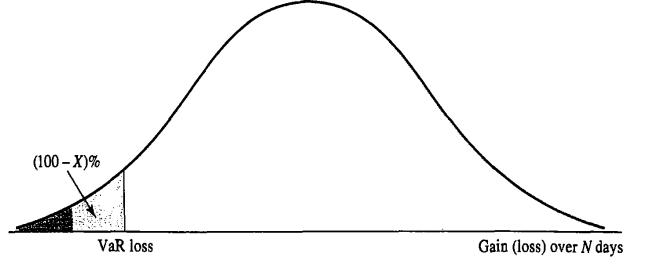
\includegraphics[width=0.5\textwidth]{Images/Image 1.png}
  \caption{The Value at Risk (VaR) is calculated from the probability distribution of the variations in the portfolio's value, where gains are represented as positive values and losses as negative. The confidence level for this calculation is set at X\%.[\ref{ref4}]}
  \label{VaR Distribution Curve}
\end{figure}

Refer to Figure~\ref{VaR Distribution Curve}, it expresses that:  
\begin{itemize}
  \item The bell-shaped curve represents the probability distribution of gains and losses for the asset or portfolio over the specified period.
  
  \item The left tail of the distribution marks the area of losses, where we can observe the VaR loss at a specific confidence level, say \( (100 - X)\% \). This tail area signifies the worst losses incurred in the historical period.
  
  \item The point where the left tail cuts the horizontal axis (gain/loss over N days) corresponds to the VaR at the chosen confidence level. For example, if \( X \) is 95, then the VaR would represent the maximum expected loss over the N days period that only 5\% of the time is expected to be exceeded.
  
  \item The graph assumes that the past can be a predictor of future risk, thus the frequency and magnitude of historical losses are directly used to estimate the VaR.
\end{itemize}

In the future, I could also use extreme value theory (EVT) to smooth our the distribution, which would allow for a more accurate estimation of the VaR, as it would allow for a better estimation of the tail of the distribution, which is where the worst losses are.[\ref{ref6}]\\\vspace{0.3cm}

\subsection{Model Building (Variance-Covariance)}

The Variance-Covariance method, used in this analysis for Value at Risk (VaR) calculation, is based on the assumption of normally distributed market returns. The key steps in the model are as follows:

\begin{enumerate}
    \item \textbf{Data Collection:} Historical price data of the asset is collected for a specified time period once again. This can be done using an API or through a CSV file.
    \item \textbf{Calculate Daily Returns:} Daily returns are computed as the percentage change in the adjusted closing prices of the stock.
    \item \textbf{Statistical Analysis:} The mean and standard deviation of the daily returns are calculated to represent the average return and the volatility of the stock, respectively.
    \item \textbf{VaR Calculation:} The Value at Risk is calculated using the formula:
    \begin{equation}
      VaR = - P \times (\text{norm.ppf}(rl, \text{mean}, \text{sD}) + 1) 
      \label{eq:Variance-Covariance VaR}
    \end{equation}
    where:
\begin{itemize}
    \item \( P \) represents the total value of the portfolio.
    \item \( \text{norm.ppf} \) is a function from the \texttt{scipy.stats} library that calculates the inverse of the cumulative distribution function (CDF) of the normal distribution, also known as the Percent Point Function (PPF).
    \item \( rl \) is the risk level, which corresponds to the confidence level for VaR. For example, a 95\% confidence level would use an \( rl \) of 0.05 (5\% risk level).
    \item \( \text{mean} \) and \( \text{sD} \) are the mean and standard deviation of the historical returns, respectively.
\end{itemize}
\end{enumerate}

\newpage
The Value at Risk (VaR) calculation in the Variance-Covariance method is executed using a specific equation that combines statistical measures with the portfolio value to estimate the potential loss over a specified time horizon. The equation is as follows:

\begin{enumerate}
    \item The \(\text{norm.ppf}\) function takes the risk level \( rl \), mean, and standard deviation of returns as inputs and outputs a Z-score. This score corresponds to the point on the normal distribution curve where the cumulative probability is equal to the risk level.
    \item The equation then multiplies this score with the portfolio value \( P \) and subtracts from \( P \). This represents the potential loss in value of the portfolio at the given confidence level.
    \item The addition of 1 in the formula adjusts for the fact that the \(\text{norm.ppf}\) function returns a negative value for typical VaR confidence levels. This is because the function calculates the Z-score for the left tail of the distribution, while VaR is the loss at the right tail. The addition of 1 converts the negative value to a positive one.
\end{enumerate}

Thus, the equation calculates the VaR as the maximum expected loss over a certain period, given normal market conditions and a specified confidence level. The Variance-Covariance method is a simple yet effective approach to VaR calculation, but it does have its limitations, such as the fact that it assumes that the returns are normally distributed, which is not always the case.\\\vspace{0.3cm}


% \\\vspace{0.3cm}


\subsection{Coding VaR Methods}
To validate that I could apply the knowledge I had gained from my research, I decided to code the two methods of VaR calculation that I had researched, this being the historical simulation and model building methods. I have decided to use Python (3.11.1) as my coding language, as it is a language that I am familiar with and has a rich ecosystem of libraries that I can use to help me with the project. I also decided to use command line to display the results, as it utilises pythons inbuilt \(\text{print()}\) command to easily display variables, allowing for a quick and easy way to display the results of the VaR calculations, as well as any tests run as well. %I have also decided to use yahoo finance as my data source, as it is a free and easy to use API that allows for the collection of historical stock data, which is exactly what I need for this project.

\subsubsection{Command Line --- Historical Simulation}
I decided to get the stock data I wanted to use for this directly from \href{https://finance.yahoo.com/}{Yahoo Finance's} online website, since it would allow me to specify the days I wanted to use, as well as the stock I wanted to use. I decided to use Nike (NKE) as my stock, as it is a company that I am familiar with and I know has been around for a long time, so it would have a lot of historical data to use. I decided to use the last 500 days of data, as it would allow for a good amount of historical stock data coverage, but not too much that it would take a long time to run.\\\vspace{0.3cm}

To start, I imported the libraries I would need, this being \texttt{numpy} and \texttt{csv}. I then created an empty array called \texttt{closes}, which would be used to store the closing prices of the stock. I then opened the CSV file that I had downloaded from Yahoo Finance, and used a \texttt{for} loop to iterate through each row of the CSV file, adding the closing price of the stock to the \texttt{closes} array.\texttt{diffs} array, this being stored in the 6th column of the CSV file.\\\vspace{0.3cm}
\begin{verbatim}
  closes = np.array([])
  with open('NKE.csv', 'r') as file:
      reader = csv.reader(file)
      for row in reader:
          closes = np.append(closes, float(row[5]))
  \end{verbatim}

I then created an empty array called \texttt{diffs}, which would be used to store the percentage differences of the closing prices of the stock, followed by a \texttt{for} loop to iterate through each element of the \texttt{closes} array, calculating said percentage difference between the current element and the previous element, then adding it to the \texttt{diffs} array. Finally, I used the \texttt{np.percentile()} function to calculate the 5th percentile of the \texttt{diffs} array, which would be the VaR for the portfolio (this meaning I didn't need to manually order it to find the 25th worst case result result, I can just use this useful function). I multiplied this by the portfolio value, which in this case was 100,000,000, to get the VaR for the portfolio and then multiplied this by -1, as VaR is always represented as a positive value, to get the final VaR value.\\\vspace{0.3cm}

  \begin{verbatim}
    diffs = np.array([])
    for i in range(1, len(closes)): 
        diffs = np.append(diffs, (closes[i]/closes[i-1] - 1))
    print("500 Day stock history, for 1 day time horizon, 95% certainty, 
           Portfolio of 100,000,000, VaR for the 23/10/2023: £" + 
           str(round(np.percentile(diffs, 5)*100000000*-1, 3)))
    \end{verbatim}

This results in this output, which appears to be a reasonable VaR result. \\\vspace{0.3cm}

  \begin{figure}[h]
    \centering
    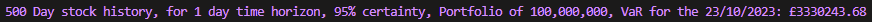
\includegraphics[width=1\textwidth]{Images/Historical Command Line Result.png}
    \caption{Historical Simulation VaR Result}
    \label{fig:Historical Command Line Result}
  \end{figure}

For this project, I did not look up any online VaR results for this stock or any other further stock used, since I believe the methods were robust enough to be reliable. Since I also create multiple methods for calculating VaR, I was able to cross-reference them with each other, with them mostly showing similar results for the same stock, so I am confident that 
these are accurate VaR predictions.

\subsubsection{Command Line -- Model Building  (Variance-Covariance)}\label{Command Model}

To begin with this method, I discovered that I could import the historical stock price data conveniently by using the \href{https://pypi.org/project/yfinance/}{yfinance} package, which provides a convenient way to download financial market data from Yahoo Finance directly into Python. I selected Nike (NKE) as the target stock so I could compare it to the previous result given by Historical Simulation. A time span of the last 500 trading days was once again chosen to balance between a sufficient data sample size and computational efficiency, as well as for comparative reasons.\\\vspace{0.3cm}

The first step was to import the necessary libraries and download the stock data using the \texttt{yf.download()} function, one of these additional libraries being scipy, which is a used for scientific and technical computing, due to it allowing the user to manipulate and visualize data with a wide range of high-level commands, one of such being the \texttt{norm.ppf()} function, which is used to calculate the inverse of the cumulative distribution function (CDF) of the normal distribution, also known as the Percent Point Function (PPF) that I will need to utilise in a future step. I then discovered that you can use the inbuilt \texttt{pct\_change()} function to calculate the daily returns/percentage changes for the whole data set, which is a much more efficient way of doing it than the method I used for Historical Simulation. I also used the \texttt{dropna()} function to remove any missing values from the data set, in case using the API rather then the CSV could cause this issue.\\\vspace{0.3cm}

\begin{verbatim}
  from scipy.stats import norm
  import yfinance as yf
  
  stock = yf.download('NKE', dt.datetime(2021, 10, 26), dt.datetime(2023, 10, 24))
  closeDiffs = stock['Adj Close'].pct_change()
\end{verbatim}

I then proceeded to define the necessary variables to calculate the VaR, following the formula outlined in Equation~\ref{eq:Variance-Covariance VaR}. The portfolio and risk level were set to 100,000,000 and 0.05 (5\%) respectively, since these were the value's used in Historical Simulation, then the mean was calculated using the \texttt{np.mean} function, followed by the standard deviation using the \texttt{np.std} function.\\\vspace{0.3cm}

\begin{verbatim}
  portfolio = 100000000
  rlPercent = 0.05
  mean = np.mean(closeDiffs)
  sD = np.std(closeDiffs)
\end{verbatim}

Finally, calculating the VaR result takes place with the negative portfolio value multiplied by the \texttt{norm.ppf()} function, which takes the risk level, mean, and standard deviation of returns as inputs and outputs a Z-score, which corresponds to the point on the normal distribution curve where the cumulative probability is equal to the risk level, giving us the VaR estimation.\\\vspace{0.3cm}

\begin{verbatim}
  print("500 Day stock history, for 1 day time horizon, 95% certainty, 
         Portfolio of 100,000,000, VaR for the 23/10/2023: £" + 
         str(round(-portfolio*(norm.ppf(rlPercent, mean, sD)), 3)))
\end{verbatim}

The output of this computation provides a VaR estimate under the assumption of normally distributed returns and a linear correlation between the assets. This assumption is a of course a simplification and might not hold during periods of financial turmoil, which I acknowledge as a limitation of the model, but for this data it is acceptably accurate.\\\vspace{0.3cm}

\begin{figure}[h]
  \centering
  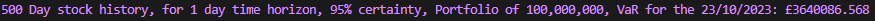
\includegraphics[width=1\textwidth]{Images/Variance-Covariance Command Line Result.png}
  \caption{Variance-Covariance VaR Result}
  \label{fig:Variance-Covariance Command Line Result}
\end{figure}

As you can see, the VaR result is very similar to the one calculated using Historical Simulation, which is a good sign that both methods are accurate. But how do I check the validity of both methods/models?

\subsection{Back-Testing}
So for the methods that I had already coded, I had achieved VaR estimations, but I had no way of validating how accurate they were, which is where back-testing comes in. Back-testing is a way of testing the accuracy of a model by using historical data to see how well it would have predicted the actual results. For example, if I had a model that predicted the weather, I could use back-testing to see how accurate it was by using historical weather data to see how well it has predicted the weather correctly in the past\\\vspace{0.3cm}

To achieve this, you need to see how many times you model has previously predicted the correct VaR, or more so, how many times they have predicted the VaR wrong. To do this, lets say you have 500 days of historical data, and you want to see how many times your model has predicted the VaR wrong for a 1 day time horizon, 95\% certainty, and a portfolio of 100,000,000. 
You would first need to take a portion of the data, lets say the first 50 days, and calculate the VaR for it using the model. You would then compare this VaR result to the actual value that the portfolio lost/gained from the 50th day to the 51st day, thus seeing if the model predicted the VaR correctly. This would then continue, keeping the 50 day data span, but moving it along by 1 day each time, so the next data span would be from the 2nd day to the 51st day, then the 3rd day to the 52nd day, and so on, until you reach the end of the data set. This can be seen in Figure~\ref{fig:Back-Testing} below.\\\vspace{0.3cm}

\begin{figure}[h]
  \centering
  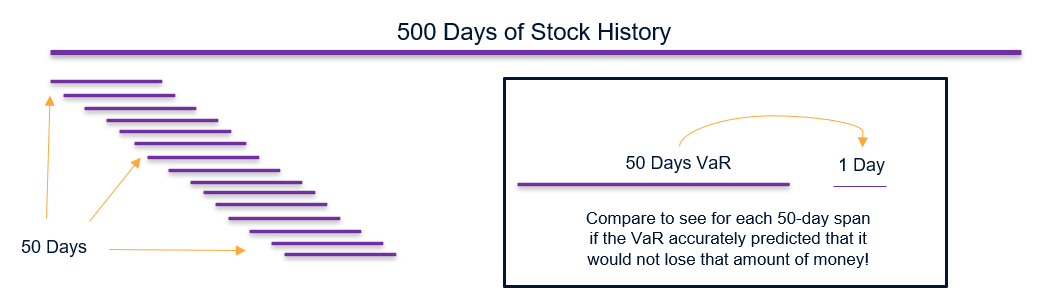
\includegraphics[width=1\textwidth]{Images/Back-Testing.png}
  \caption{Back-Testing Diagram (Source: My Presentation Powerpoint)}
  \label{fig:Back-Testing}
\end{figure}

Every time one of these spans creates a VaR that fails to accurately predict the next days loss, you would make note of it and add it to a counting total. This total can then be utilised with p-values. A p-value is a statistical measure that helps to determine the significance of the results obtained from a hypothesis test. In the context of back-testing, the null hypothesis typically states that the model's predictions are correct, and the alternative hypothesis suggests that the model's predictions are not accurate. A low p-value indicates that the observed data is unlikely under the null hypothesis, leading to its rejection in favour of the alternative hypothesis. So for our VaR back-testing, a low p-value would suggest that the model's performance is not as good as predicted, potentially failing to capture the risk adequately.

To do this within Python whilst leading on from our previous two coded methods, I added the following codee to the end on both models. It creates a variable called \texttt{count}, which is used to count the number of times the model has predicted the VaR incorrectly, and a variable called \texttt{adjust}, which is used to adjust the data span to be used for the VaR calculation, this being 10\% of the data set. It then creates a \texttt{for} loop, which iterates through each day of the data set, calculating the VaR for the data span, then comparing it to the actual value that the portfolio lost/gained from the last day of the data span to the next day, thus seeing if the model predicted the VaR correctly. This will repeat for the length of the entire historical data history, minus the span adjust and minus 1 as well, since you would need to compare 449--499 day VaR to day 449--500's return. The next day return is also multiplied by -1, so it accounts so that the losses are positive like the VaR estimations, making it easy to compare if one is incorrectly larger then the other. If the VaR was predicted incorrectly, the \texttt{count} variable is increased by 1.\\\vspace{0.3cm}

\begin{verbatim}
  count = 0
  adjust = int(len(stock)/10)
  for i in range(1, len(stock) - adjust - 1):
      backTest = stock['Adj Close'].pct_change()[i:i+adjust]
      if Historical Simulation:
          VaR = np.percentile(backTest, rlPercent)*portfolio*-1
      else: #Model Building
          VaR = -portfolio*(norm.ppf(rlPercent, mean, sD))
      nextDay = stock['Adj Close'].pct_change()[i+adjust:i+adjust+1].values[0]
      nextDay = nextDay*portfolio*-1
      if nextDay > VaR:
          count += 1
\end{verbatim}

 Next, I compute the p-value using the cumulative distribution function (CDF) of the binomial distribution, which in turn calculates the probability of observing a certain number of VaR exceedances (or fewer) given the expected number of exceedances under the model's assumptions.\vspace{0.3cm}
 
 \begin{verbatim}
  pValue = binom.cdf((len(stock)-adjust)-count,len(stock)-adjust,1-rlPercent/100)
  \end{verbatim}

 The parameters for the \texttt{binom.cdf} function are as follows:

\begin{itemize}
    \item The number of successes, which is the total number of days minus the adjustment for the data window and the count of exceedances.
    \item The number of trials, which is the length of the stock data minus the adjustment for the data window.
    \item The probability of success on each trial, which is 1 minus the risk level percentage divided by 100, reflecting the confidence level of the VaR estimate.
\end{itemize}

The calculated p-value is then compared to the risk level percentage to determine the statistical significance. If the p-value is greater than the risk level percentage, the model passes the back-test, indicating that the number of VaR exceedances is within acceptable limits of the model's predictions. Conversely, a p-value lower than the risk level percentage suggests that the model's poor predictive performance is statistical significance, and it fails the back-test.[\ref{ref11}]

\begin{verbatim}
if pValue > rlPercent/100:
    print("Back Test: PASSED with " + str(round(pValue*100, 0)) + 
    "% statistical significance level (p-value)")
else:
    print("Back Test: FAILED with " + str(round(pValue*100, 0)) + 
    "% statistical significance level (p-value)")
\end{verbatim}

By utilizing p-values, we can assign a level of confidence to our back-testing results, supporting the validation process of our VaR model. It enables us to make informed decisions about the model's reliability and whether it can be trusted for making future risk assessments. It help provide a quantitative method to validate the accuracy of VaR models, ensuring that risk managers and financial analysts can rely on the model's predictions to make critical decisions. In the future, along a set of portfolio's with multiple stocks within, I could perform multiple back test on multiple stocks using both VaR, and form a statistical conclusion on how many time each model fails the p-value back-testing, thus seeing which model is more reliable and should possibly be used in further graphical builds, although I have not touched on Monet Carlo simulation yet, which could be far more accurate then either of these two methods, so I will have to see how my research into it goes.[\ref{ref11}]

\begin{figure}
  \centering
  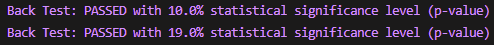
\includegraphics[width=0.7\textwidth]{Images/Back-Testing Results.png}
  \caption{Results using Tesco stock data, for Historical Simulation followed by Model Building.}
  \label{fig:Back-Testing Results}
\end{figure}

\subsection{Combining Implementations}
Before I decided to embark on the creation of any of my graphical elements, I thought it would be good to have some way to test my VaR models on different single stocks, so I could see a range of results, and better gauge the consistency levels of my back-tests, as well as also being able to simple see more VaR results then just what I had seen so far. I created a fully functioning command line program that allows the user to select a stock from the FTSE100 list (I chose this as I do not have a wide knowledge of stock lists, but since I knew of this one already and all the stocks on it are significant, it would be good to implement), enter a given portfolio value that they would have invested within this one particular stock, and then select a time horizon and confidence level for the VaR calculation. It would then give them 3 options for how much historical data they would want to use, either 100, 500 or they could input their own dates, and it would finally ask what model they would like to compute the VaR estimation with, either Historical Simulation or Model Building. It would compute the VaR and then display the result, as well as display the p-value back-testing result.\\\vspace{0.3cm}

Since the code for this is just a large and robust amount of verification and input statements, I will not include it in this report, but I will display a full interaction in figure~\ref{fig:Single Stock VaR}. I used pandas to retrieve the FTSE100 from Wikipedia, pandas being a powerful data manipulation library in Python, allowing for web scraping, reading and writing data, which I utilised it for in this case. Everything else included within the code has been covered within previous pages within this chapter. Full interaction found on the next page:

\begin{figure}
  \begin{verbatim}
    WELCOME TO THE VAR CALCULATOR
    -----------------------------
    Which companies stock would you like to calculate the VaR for?
    1 - 3i
    2 - Admiral Group
    3 - Airtel Africa
    ...
    40 - Haleon
    41 - Halma plc
    42 - Hargreaves Lansdown
    43 - Hikma Pharmaceuticals
    44 - Howdens Joinery
    ...
    97 - Vodafone Group
    98 - Weir Group
    99 - Whitbread
    100 - WPP plc
    Enter the number of the company: 42
    Enter the portfolio value (£): 100000000
    Enter the risk level percentage (1%, 5%, etc.): 5
    Enter the time horizon (Max: 100 days): 1
    How many days of historical data would you like to use, 
    or would you like to choose your own date boundaries?
    1. 100 days
    2. 500 days
    3. Choose your own
    Enter the number of your choice: 2
    [*********************100%%**********************]  1 of 1 completed
    Would you like to calculate VaR using Historical Simulation, 
    or using Model Building/Variance-Covariance (H/M): m
    
    VaR is: £5,818,845.68
    Back Test: PASSED with 32.0% statistical significance level (p-value)
  \end{verbatim}
  \caption{Console output of the Single Stock VaR.py program.}\label{fig:Single Stock VaR}
\end{figure}

 I have neglected to mention how the Time Horizon in handled within this program. The best way to show how it is handled would be to quote from reference [\ref{ref6}] --- \textit{Options, Futures, and Other Derivatives.} by John C. Hull, which states:

 \begin{quote}
  VaR has two parameters: the time horizon \( N \), measured in days, and the confidence level \( X \). In practice, analysts almost invariably set \( N = 1 \) in the first instance. This is because there is not enough data to estimate directly the behavior of market variables over periods of time longer than 1 day. The usual assumption is: 
  \begin{equation}
    N\text{-day VaR} = \text{1-day VaR} \times \sqrt{N}
    \label{eq:Time Horizon}
  \end{equation}
  This formula is exactly true when the changes in the value of the portfolio on successive days have independent identical normal distributions with mean zero. In other cases, it is an approximation.
\end{quote}
  
  Since VaR is scaled with time due to volatility. Volatility tends to be proportional to the square root of time.
  \begin{equation}
    \text{Volatility(Time)} = \text{Volatility(One Period)} \times \sqrt{\text{Time Horizon}}
    \label{eq:Volatility}
  \end{equation} 

  Since we are dealing with the other cases frequently throughout the use of the VaR Models used within the programs, I utilise the formula \ref{eq:Time Horizon} above to accommodate for the VaR value over a given time period, by multiplying the VaR by the square root of the given time horizon, which is why the user is asked to input the time horizon in days, and not in years or months, this providing sufficient estimations so far.

% \subsubsection{Multiple Stocks}
\newpage
\section{Chapter 3 --- Graphical User Interface}

\subsection{What is Kivy?}
Kivy \href[page=1]{https://kivy.org/#home}{(https://kivy.org/)}is an open-source Python library for developing multitouch application software with a natural user interface (NUI). It is highly versatile and can run on various operating systems, including Windows, macOS, Linux, Android, and iOS\@. This cross-platform compatibility is due to Kivy's use of OpenGL ES 2, allowing it to render consistent graphics across all supported platforms.[\ref{ref9}] Kivy is also free to use, even for commercial purposes, as it is distributed under the MIT license.\\\vspace{0.3cm}

Kivy's compatibility with multiple operating systems makes it an excellent choice for financial software development. The ability to write code once and deploy it on various platforms without modification is particularly advantageous in a financial context, where users may access software from different devices.

\begin{itemize}
    \item \textbf{Cross-Platform:} Kivy apps can run on desktop and mobile devices, enhancing accessibility for users who need to monitor financial markets or run VaR calculations on the go.
    \item \textbf{Pythonic Nature:} Given that Python is a leading language in financial modelling due to its simplicity and the powerful data analysis libraries available, Kivy integrates well within the Python ecosystem, as well as it being the chosen language for this project.
    \item \textbf{Graphics Engine:} Kivy's graphics engine is built over OpenGL ES 2, providing the capability to handle intensive graphical representations, which is essential for visualizing complex financial data that I will want to do in the future.
\end{itemize}

Developing financial software with Kivy brings several benefits:

\begin{itemize}
    \item \textbf{Rapid Development:} Kivy's straightforward syntax and powerful widgets allow for rapid development of prototypes and software, which is crucial in the fast-paced environment of financial markets.
    
    \item \textbf{Multitouch Support:} The library's inherent support for multitouch can be leveraged to create interactive financial dashboards, enhancing data exploration and manipulation for important tasks such as risk analysis which we will want to use it for.[\ref{ref9}] 
    
    \item \textbf{Customizable UI:} Kivy provides the tools to create a highly customizable user interface (UI), enabling the development of aesthetic financial applications tailored to the specific needs of financial analysts.
    
    \item \textbf{Community and Support:} Kivy has a growing community and good documentation, which will be highly useful for me as a beginner to the library.
\end{itemize}

Kivy presents itself as a robust framework for financial software development. Its compatibility with different operating systems, ease of operation within Python, and the capability to create sophisticated UIs make it an appealing choice for developers such as myself to use when creating financial applications, especially when catered for VaR analysis and other risk management tools, which is why I've chosen to use it for this project for the GUI.\@

\subsection{Conceptualisation of Initial Design Ideas}

The initial design phase of the Value at Risk (VaR) calculation tool will focus on creating a tool that will allow the user to interact with it in an efficient and effective manor, with less of an emphasis on a visually pleasing design, more on practicality for what has been researched and commented on so far. I had an idea in mind for what I wanted to initially be able to create, so I decided to create a design sketch (Figure~\ref{fig:InitialDesignSketch}), which reflects an early conceptualization of the interface, emphasizing simplicity and functionality.

\begin{figure}[h]
  \centering
  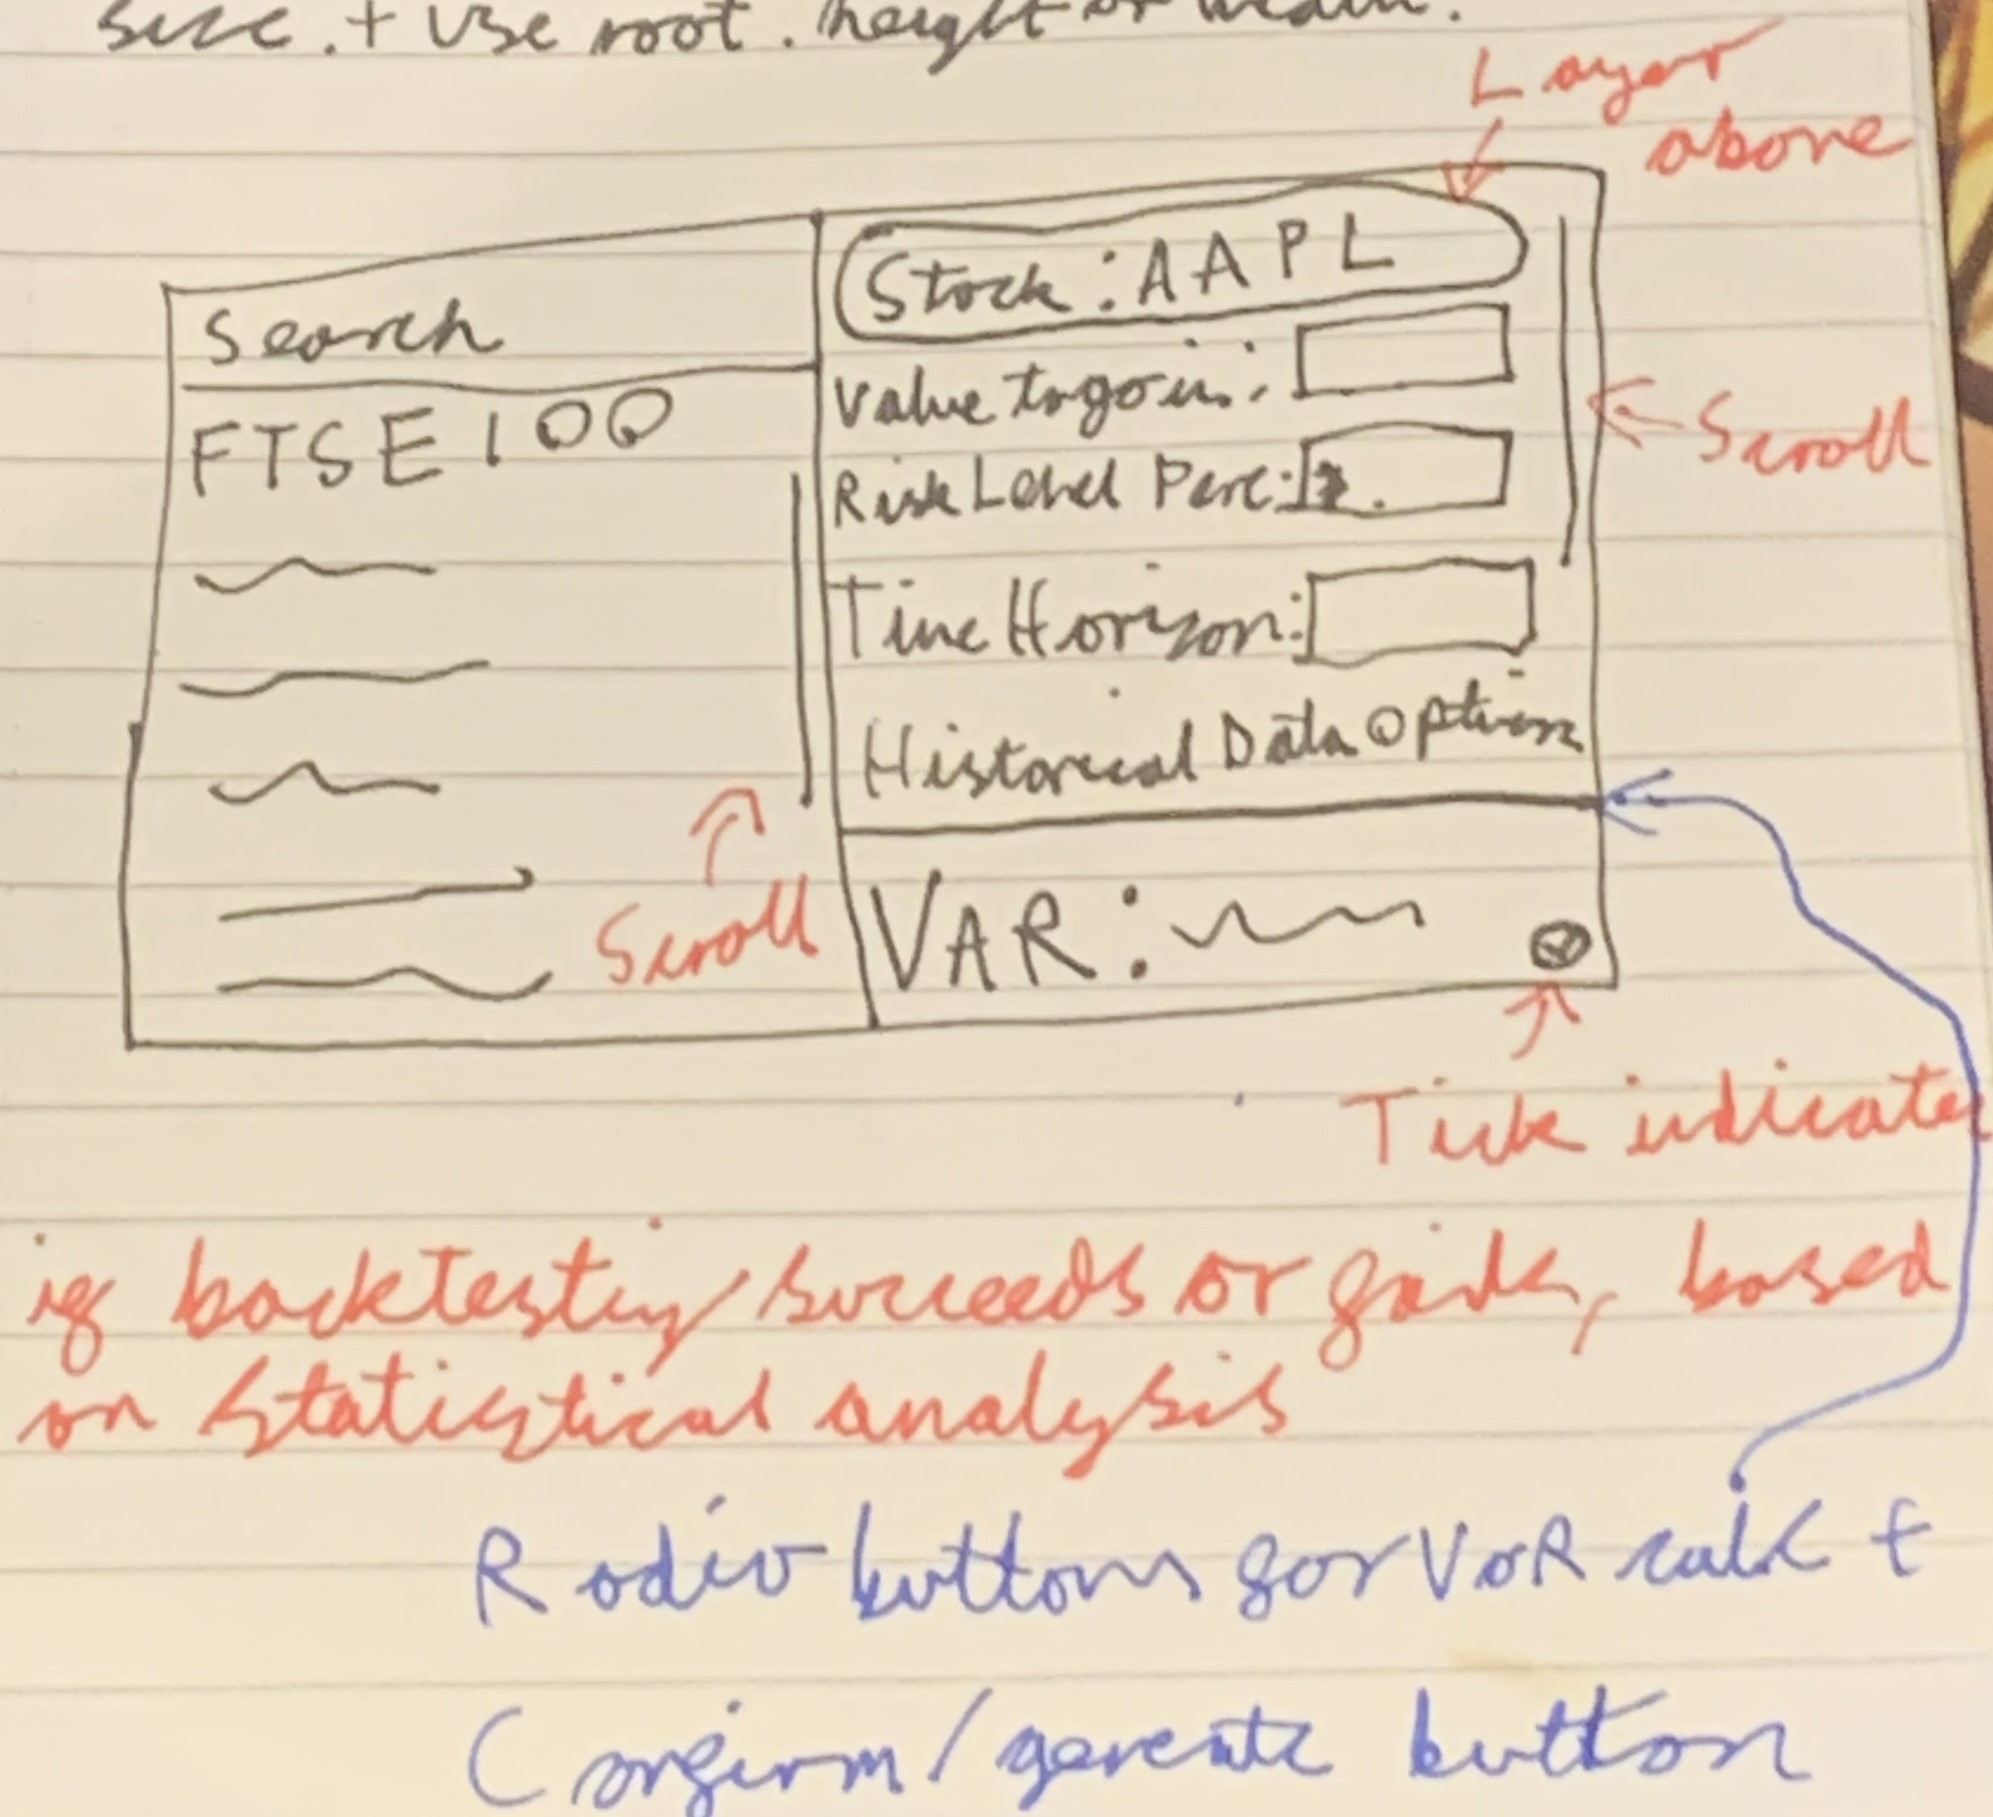
\includegraphics[width=0.7\textwidth]{Images/Initial Design Sketch.jpg}
  \caption{Initial GUI Design Sketch}
  \label{fig:InitialDesignSketch}
\end{figure}

The layout was envisioned to comprise of two main sections: a search and selection panel on the left and an input/detail panel on the right. The search panel allows users to filter and select stocks from the FTSE100 to then be used on the right, as well as search for any stock that they want from an autocomplete database. The detail panel on the right is structured to enable users to specify parameters for the selected stock, such as portfolio value, risk level percentile, time horizon and what VaR model you want to use. A scroll feature could also be implemented to accommodate future desired adjustable parameters, such as historical data options. Below the scroll is a fixed section that will display the final VaR after the rest of the informational parameters have been interacted with/data has been submitted into them. There will also be a tick to indicate if back-testing's hypothesis through statistical analysis had been rejected, this influencing if this model with this stock passes.\\\vspace{0.3cm}

A key feature highlighted in the sketch is the inclusion of the layered "current stock" display in the top right, as it lets the users easily see what they have selected, whilst also letting the scroll move underneath it, helping the program look and act dynamically. Additionally, a tick indicator was conceptualized to provide immediate visual feedback when back-testing succeeds or fails, based on statistical analysis (p-values), enhancing the user's understanding of the model's performance, showing evidence of system status. The design also incorporates radio buttons for VaR calculation modes for historical and model-based approaches, allowing for quick toggling between different methods whilst still maintaining the other pre-selected parameters.\\\vspace{0.3cm}

This initial design was guided by principles of user centered design (UCD) best practices, aiming to streamline the complex process of risk analysis into a manageable and approachable workflow for end-users. Each element was chosen for its potential to make the software accessible to both novice and experienced users, allowing for ease of user regardless of skill level.\\\vspace{0.3cm}

The conceptualisation phase was pivotal in laying the groundwork for the subsequent development of this GUI. It helped me visualise how it needed to look and how the interactions would have to take place, so even if the final result wasn't visually the same, it still provided an excellent user story for how it needed to perform.

\subsection{Initial GUI Creation}
Before my initial creation, I briefly followed the book [\ref{ref9}], \textit{Kivy - Interactive Applications and Games in Python - Second Edition} by Roberto Ulloa, which I have referenced in my bibliography, as it's a very useful book for learning the basics of Kivy, and I would highly recommend it to anyone who wants to learn the library.

\subsubsection{First Iteration}
Since the book taught me to separate the GUI into two files, I have done so for my baseline of the application, these files  being the .py file, which contains the code for the GUI, and the other being the .kv file, which contains the layout and styling of the GUI, I will be explaining the code for both of these files, as well as the code for the main.py file, which is the file that runs the GUI.\@\\\vspace{0.3cm}

The Python script `Initial Design Test.py' serves as the backbone of the application. Utilizing Kivy's standard libraries, the script defines my ApplicationView class, which inherits from Kivy's BoxLayout to establish the fundamental structure of the GUI:

\begin{verbatim}
class ApplicationView(BoxLayout):
    stockList = ObjectProperty(None)
    userInputs = ObjectProperty(None)
    ...
    def populateList(self):
        ...
    def populateInputs(self):
        ...
\end{verbatim}

The `ApplicationView' class is integral to the GUI, as it initializes the user interface and binds the graphical components to the backend logic. The ObjectProperty instances `stockList' and `userInputs' are object placeholders for dynamic python elements within the GUI.\@ The methods `populateList' and `populateInputs' are responsible for filling these placeholders with actual content — in this case, labels representing stock data and text input fields for user parameters, respectively.\\\vspace{0.3cm}

The layout and styling of the GUI are defined in the Kivy language file `IDT.kv', which allows for a clear separation of the interface design from the logic of the application:

\begin{verbatim}
<ApplicationView>:
    orientation: 'horizontal'
    BoxLayout:
        orientation: 'vertical'
        ...
        ScrollView:
            ...
\end{verbatim}

This .kv file outlines two main sections in a horizontal arrangement — a searchable stock list and a detailed input area for configuring VaR parameters. The use of ScrollView elements ensures that the content is accessible even when it exceeds the screen space. This design decision was made to enhance the application's scalability and to provide a seamless user experience.\\\vspace{0.3cm}

The `populateList' and `populateInputs' functions demonstrate the dynamic nature of the interface. They are called upon initialization to populate the GUI with interactive elements:

\begin{verbatim}
def populateList(self):
    for i in range(100):
        self.stockList.add_widget(Label(...))
        
def populateInputs(self):
    for i in range(20):
        self.userInputs.add_widget(Label(...))
        self.userInputs.add_widget(TextInput(...))
\end{verbatim}

These functions are responsible for creating the labels and text input fields that are displayed in the GUI.\@ The labels are populated will hopefully be populated stock data, and the text input fields will be used to configure VaR parameters.  This approach allows for the creation of a scalable interface that can be easily adapted to accommodate additional stocks and parameters in the future, once they are implemented.\\\vspace{0.3cm}

Upon executing the `Initial Design Test.py' script, the Kivy application builds the GUI based on the defined classes and .kv file, initiated by the following code:

\begin{verbatim}
if __name__ == '__main__':
    IDTApp().run()
\end{verbatim}

\begin{figure}[h!]
  \centering
  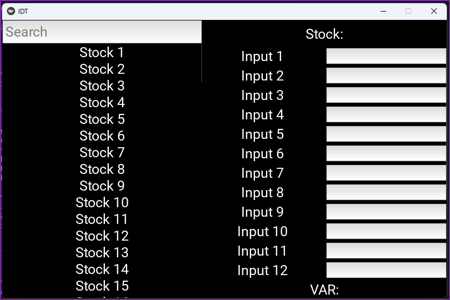
\includegraphics[width=0.8\textwidth]{Images/Initial Design Test Image 1.png}
  \caption{Initial Design Test - First Iteration}
  \label{fig:Initial Design Test - First Iteration}
\end{figure}

\newpage

\subsubsection{Final Iteration}

\subsection{Completed Initial Design}
For my final iteration of my first design, I took all of the elements that were explored within the Combining Implementations chapter, and implemented them into the GUI, as well as adapting some of the old features so they could work in the boundary of what I was able to achieve.


\subsubsection{Enhanced Application Structure}
The `ApplicationView` class has been expanded to include new properties and functionalities that support a richer user experience and more sophisticated data analysis capabilities:

\begin{verbatim}
class ApplicationView(BoxLayout):
    portfolio = 100000000
    rlPercent = 5
    timeHori = 1
    simMethod = "Historical"
    currentTicker = ""
    ...
\end{verbatim}

These new properties include a default portfolio value, risk level percentage, time horizon for analysis, simulation method preference, and the currently selected stock ticker. This setup allows for a dynamic and customizable analysis based on user inputs.

\subsubsection{Dynamic Stock List Generation}
The method `populateList` dynamically generates a list of stocks from the FTSE 100 index, allowing users to select a company for analysis:

\begin{verbatim}
def populateList(self):
    for i in range(len(ftse100)):
        button = Button(text=ftse100['Company'][i], ...)
        button.bind(on_release=lambda btn, i=i: ...)
        self.stockList.add_widget(button)
\end{verbatim}

This code snippet showcases the application's ability to fetch and display a list of companies from a live data source (Wikipedia), with each company represented as a button within the user interface.

\subsubsection{Value at Risk (VaR) Calculation}
The `generateVaR` method calculates the Value at Risk for the selected stock, using either historical data or a model simulation approach:

\begin{verbatim}
def generateVaR(self):
    ...
    stock = yf.download(self.currentTicker, startDate, endDate).tail(500)
    ...
    if self.simMethod == "Historical":
        VaR = np.percentile(closeDiffs, self.rlPercent)...
    else:
        VaR = (-self.portfolio*norm.ppf(self.rlPercent/100, ...)...
    ...
    setattr(self.valAtRisk, 'text', " VaR: £" + VaR)
\end{verbatim}

This function demonstrates complex financial analysis by downloading stock data using `yfinance`, calculating percentage changes in the stock's closing price, and determining the VaR based on the user's selected risk assessment method.

\subsubsection{Back-testing Functionality}
The `backTest` method evaluates the performance of the VaR calculation against historical data to assess its accuracy:

\begin{verbatim}
def backTest(self, stock):
    ...
    for i in range(1, len(stock) - adjust - 1):
        ...
        if VaR > nextDay:
            count += 1
    ...
    if pValue > self.rlPercent/100:
        ...
    else:
        ...
\end{verbatim}

This section of the code uses historical stock price data to perform a back-test, comparing calculated VaR values against actual market movements to generate a statistical p-value representing the model's reliability.

\subsubsection{User Input Handling and Validation}
The application includes mechanisms to handle and validate user inputs, ensuring that the analysis is based on accurate and realistic parameters:

\begin{verbatim}
def validateInput(self, current, varName, maxVal):
    ...
    if varName == 'portfolio':
        ...
    elif varName == 'rlPercent':
        ...
    else:
        ...
    self.populateInputs()
\end{verbatim}

This function validates user inputs for the portfolio value, risk level percentage, and time horizon, applying constraints and default values as necessary. It showcases the application's robust error handling and user feedback mechanisms.

\subsubsection{Kivy Layout and Styling}
The Kivy language file (.kv) defines the layout and appearance of the application, separating the design from the Python logic:

\begin{verbatim}
<ApplicationView>:
    orientation: 'horizontal'
    ...
    ScrollView:
        ...
    BoxLayout:
        ...
\end{verbatim}

This .kv file segment outlines the application's main layout, demonstrating the use of ScrollView for the stock list and BoxLayout for organizing interface elements. This separation of concerns facilitates easier maintenance and updates to the UI without altering the backend logic.

\textbf{Conclusion:}
The final iteration of the application incorporates advanced data processing, user interaction, and financial analysis features. Through detailed explanations of key code sections, we have illustrated how the application leverages Python's capabilities and Kivy's framework to provide a rich user experience and robust financial analysis tools. Further elaboration may be required to fully cover all aspects of the code's functionality and design decisions.

\begin{figure}[h!]
  \centering
  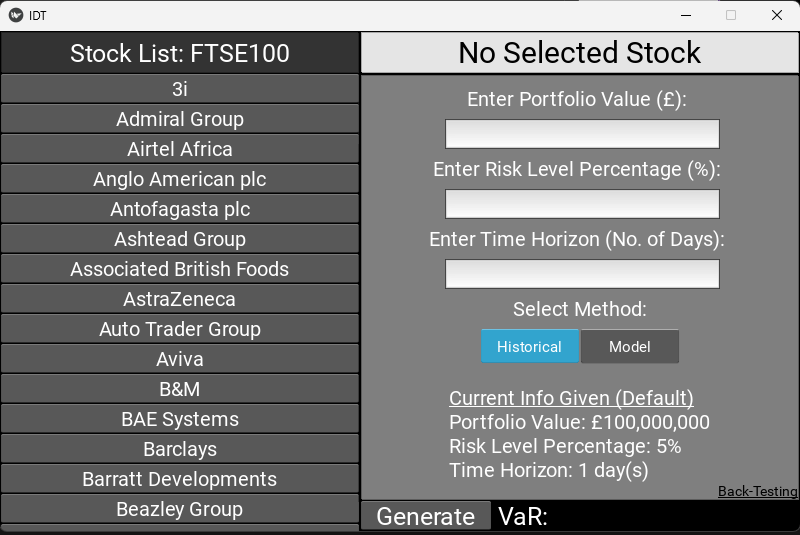
\includegraphics[width=0.8\textwidth]{Images/Initial Design Tes - Final Iteration 1.png}
  \caption{Initial Design Test - Final Iteration 1}
  \label{fig:Initial Design Test - Final Iteration 1}
\end{figure}

\begin{figure}[h!]
  \centering
  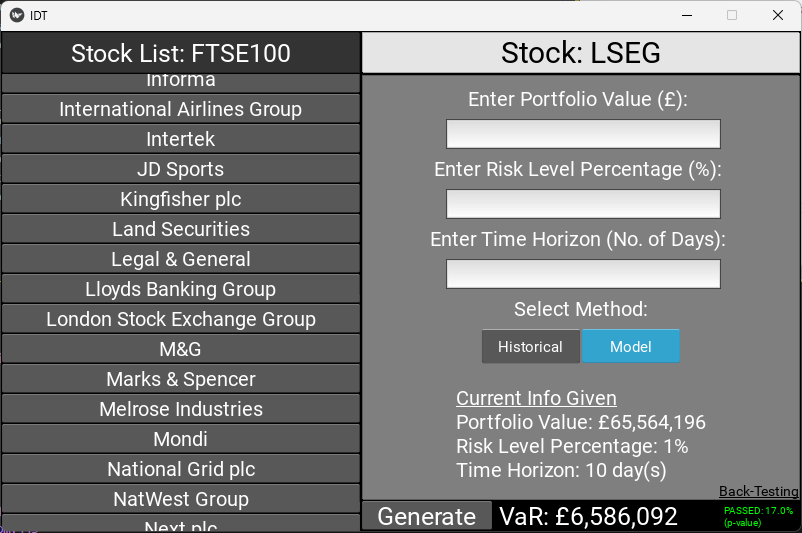
\includegraphics[width=0.8\textwidth]{Images/Initial Design Tes - Final Iteration 2.png}
  \caption{Initial Design Test - Final Iteration 2}
  \label{fig:Initial Design Test - Final Iteration 2}
\end{figure}

Youtube Video: \href{https://youtu.be/2GIWug_IESI}{Presentation Demonstration For Final Initial Design - FYP}

\subsection{Reflectional Adjustments}



\section{Chapter 4 --- Portfolio Creation}

\subsection{Monte Carlo Simulation}

Monte Carlo Simulation is arguably the most important computational technique I will need for calculating Value at Risk, since it can be utilised to perform repeated random sampling to estimate complex mathematical or physical models across a series of values. It's extremely useful in finance for the valuation of instruments, portfolios, and investments under uncertainty, since it simulates a range of possible outcomes for these random processes and proceeds to  averages the results to find a probabilistic estimation of the what the actual outcome would be.\\\vspace{0.3cm}

For these Value at Risk (VaR) calculations, Monte Carlo Simulation allows for an estimation of the potential loss in value of a whole portfolio (different to the single stock's I've been dealing with using previous methods) with any given confidence level over the specified period. It does this by simulating the returns of the portfolio across numerous simulated scenarios to create a distribution of possible outcomes, and since VaR can then be derived as a percentile of this randomly estimated distribution, such as the 5th percentile, it helps indicate that there is a 95\% confidence level that losses will not exceed this value, or an equivalently based 5\% risk level that the losses will exceed.\\\vspace{0.3cm}

It helps model the probability of different outcomes in a process that cannot easily be predicted due to the intervention of random variables, such as with multiple stocks within a stock market. The method involves generating a large number of random portfolio return paths based on historical return distributions and then determining the VaR from these simulated paths.\\\vspace{0.3cm}

Given a portfolio consisting of \(n\) assets, let \(r = (r_1, r_2, \ldots, r_n)\) denote the vector of daily returns of these assets. The return of the portfolio on any given day can be expressed as a weighted sum of the individual asset returns:

\begin{equation}
    R = w \cdot r^T
\end{equation}

where:
\begin{itemize}
  \item \(R\) is the portfolio return.
  \item \(w = (w_1, w_2, \ldots, w_n)\) is the vector of portfolio weights corresponding to each asset, stocks in our case.
  \item \(r^T\) is the transpose of the return vector.
\end{itemize}

\vspace{5cm}
When using Monte Carlo Simulation for VaR calculation, we simulate this return \(R\) for a given time horizon using the historical mean (\(\mu\)) and covariance (\(\Sigma\)) of the asset returns. For a single-day horizon, the simulated return for the portfolio can be generated from a multivariate normal distribution:

\begin{equation}
  \tilde{r} \sim \mathcal{N}(\mu, \Sigma)
\end{equation}

where:
\begin{itemize}
  \item \(\tilde{r}\) represents a vector of simulated daily returns for the portfolio assets.
  \item The process is repeated \(N\) times to generate a distribution of simulated portfolio returns.
\end{itemize}

\vspace{0.3cm}
This corresponds, based on the amount of repeated simulations \(N\) and subsequent returns \(\tilde{R}\), to the following:

\begin{equation}
    \{\tilde{R}_1, \tilde{R}_2, \ldots, \tilde{R}_N\} = \{w \cdot \tilde{r}_1^T, w \cdot \tilde{r}_2^T, \ldots, w \cdot \tilde{r}_N^T\}
\end{equation}

\vspace{0.3cm}
The VaR at a confidence level (e.g. 95\%) or equivalent risk level \(\alpha\) (e.g. 5\%) is then determined by finding the \((\alpha)\)th-percentile of this simulated portfolio returns distribution:

\begin{equation}
  VaR_\alpha = -\min \{\tilde{R} : P(R \leq \tilde{R}) \geq \alpha\}
\end{equation}

where:
\begin{itemize}
  \item \(VaR_\alpha\) is the Value at Risk at the risk level \(\alpha\). This represents the loss that is not exceeded with probability \(\alpha\), indicating a worst-case scenario within the bounds of the specified risk level.
  \item \(\tilde{R}\) represents a possible return.
  \item \(R\) is the random variable representing portfolio returns.
  \item \(P(R \leq \tilde{R})\) is the probability that the portfolio return is less than or equal to \(\tilde{R}\).
  \item \(\alpha\) is the risk level, indicating the portion of the distribution under consideration for VaR. \\For example, a confidence level of 95\%, would result in a risk level \(\alpha\) of 0.05 (5\%), reflecting the lower 5\% of the return distribution where the losses lie.
\end{itemize}

In theory, when the simulated returns are sorted in ascending order, the \((\alpha)\)-quantile is directly computed as the value at the \(N(\alpha)\)-th position in the sorted list, where \(N\) is the total number of simulations. This quantile represents the maximum expected loss at the risk level \(\alpha\), representing the worst-case scenario within the specified risk bounds over the given time horizon. For a given portfolio value \(P\), the monetary value of the VaR can be calculated as:

\begin{equation}
    VaR_{\text{Monetary}} = P \times VaR_\alpha
\end{equation}

This given mathematical framework helps underpin the Monte Carlo Simulation approach to VaR calculation, providing a probabilistic estimate of potential portfolio losses over a specified time horizon based on historical asset performance. This is what I will need to adapt to python in my subsequent program to be able to estimate VaR calculations within a portfolio of stocks.



\subsubsection{Command Line --- Monte Carlo Simulation}

Continuing on from my proof of concept programs for Historical and Method simulation, I used Yahoo Finance package again to obtain stocks from Nike (NKE), Adidas (ADS.DE), and Under Armour (UAA) over a period of 100 days. I will leverage historical price data to help model my portfolios future returns distribution. I will also be using the numpy package, since it lets me perform the random multivariate normal distribution, as well as the dot product sum between this result and my weightings. \\\vspace{0.3cm}


Firstly, I download the historical price data for the specified stocks using the \texttt{yfinance} package and subsequently  calculate the daily returns, dropping any missing values. I assign theoretical weights to each stock in the portfolio and calculate the mean and covariance of these daily returns, key inputs for the simulation.\\\vspace{0.3cm}

\begin{verbatim}
  stock = yf.download(['NKE', 'ADS.DE', 'UAA'], period='100d')
  closeDiffs = stock['Close'].pct_change().dropna()

  weighting = np.array([0.333, 0.333, 0.334])
  mean = closeDiffs.mean()
  cov = closeDiffs.cov()
  timeHori = 1
\end{verbatim}

\vspace{0.3cm}
The Monte Carlo simulation is conducted by generating random samples from a multivariate normal distribution, utilising the mean and covariance of the daily returns, simulating the portfolio's returns over the specified time horizon. The process is then repeated a large number of times to form a distribution of the portfolio's returns, in this case I opted for 10,000 simulations for the program. I initialise an empty list to store the simulated portfolio returns and iterate over the number of simulations, calculating the weighted sum of the simulated returns to represent the portfolio return for each simulation, appending these results to the list.\\\vspace{0.3cm}

\begin{verbatim}
  portfoReturns = []
  for x in range(10000):
      simReturns = np.random.multivariate_normal(mean, cov, timeHori)
      singleReturn = np.sum(simReturns * weighting)
      portfoReturns.append(singleReturn)
\end{verbatim}

\vspace{0.3cm}
Finally, I sort the simulated returns and calculate the VaR by determining the value at the specified percentile of the distribution. In this case, using the 5th percentile, a risk level of 5\%, which I then multiply by my theoretical portfolio value (100,000,000) to obtain the monetary VaR, rounded to two decimal places for logical pounds and pence articulation.\\\vspace{0.3cm}

\begin{verbatim}
  portfoReturns = sorted(portfoReturns)
  rlPercent = 0.05
  print("VaR: \pounds" + str("{:,}".format(round(-np.percentile(portfoReturns, 
                                            100 * rlPercent)*100000000, 2))))
\end{verbatim}

\vspace{0.3cm}
Using this methodology, I can provide a robust framework for estimating the VaR for any portfolio I chose to create in the future, adapting to various market conditions, and through the use of this simulation, capturing the inherent uncertainties and correlations between these assets.


\subsection{Kivy Screen Manager}
I knew that next I would want to implement what I had learnt about Monte Carlo Simulation into my GUI, but my current deliverable couldn't handle multiple stocks being selected at the same time, let alone the calculation of the VaR for them all, as it was only designed for single stock VaR calculations. I figured the best way to implement this be to add more sections to my program that can actually handle these multiple stocks needed, in essence, I needed to have the ability to create a portfolio. And since this was building towards my final deliverable, I knew I wanted to produce something that would adhere to the industry standards that I was creating my software for.\\\vspace{0.3cm}

Subsequently, upon researching more into the capabilities of kivy and its framework using the online Kivy documentation [\ref{ref13}], I discovered the Kivy Screen Manager, a powerful tool that allows for the creation of multiple screens within a single application, each screen able to be utilised as a different section and form of functionality within the program. This was perfect for what I wanted to achieve, the ability to have multiple screens represented within one application, bouncing between the different options depending on what you need to do, possibly allowing for communication between screen adding to a more in-depth functionality provided by my program. It also allowed for impressive transitional animations between defined screens, an impressive gif showcasing this being found on the main page for it within the documentation. With this, I knew I had to plan out and draft what I initially needed for my subsequent final deliverable, so just as I had done with my previous design, I drew what I envisioned in the figure below:\\\vspace{0.3cm}

\begin{figure}[h]
  \centering
  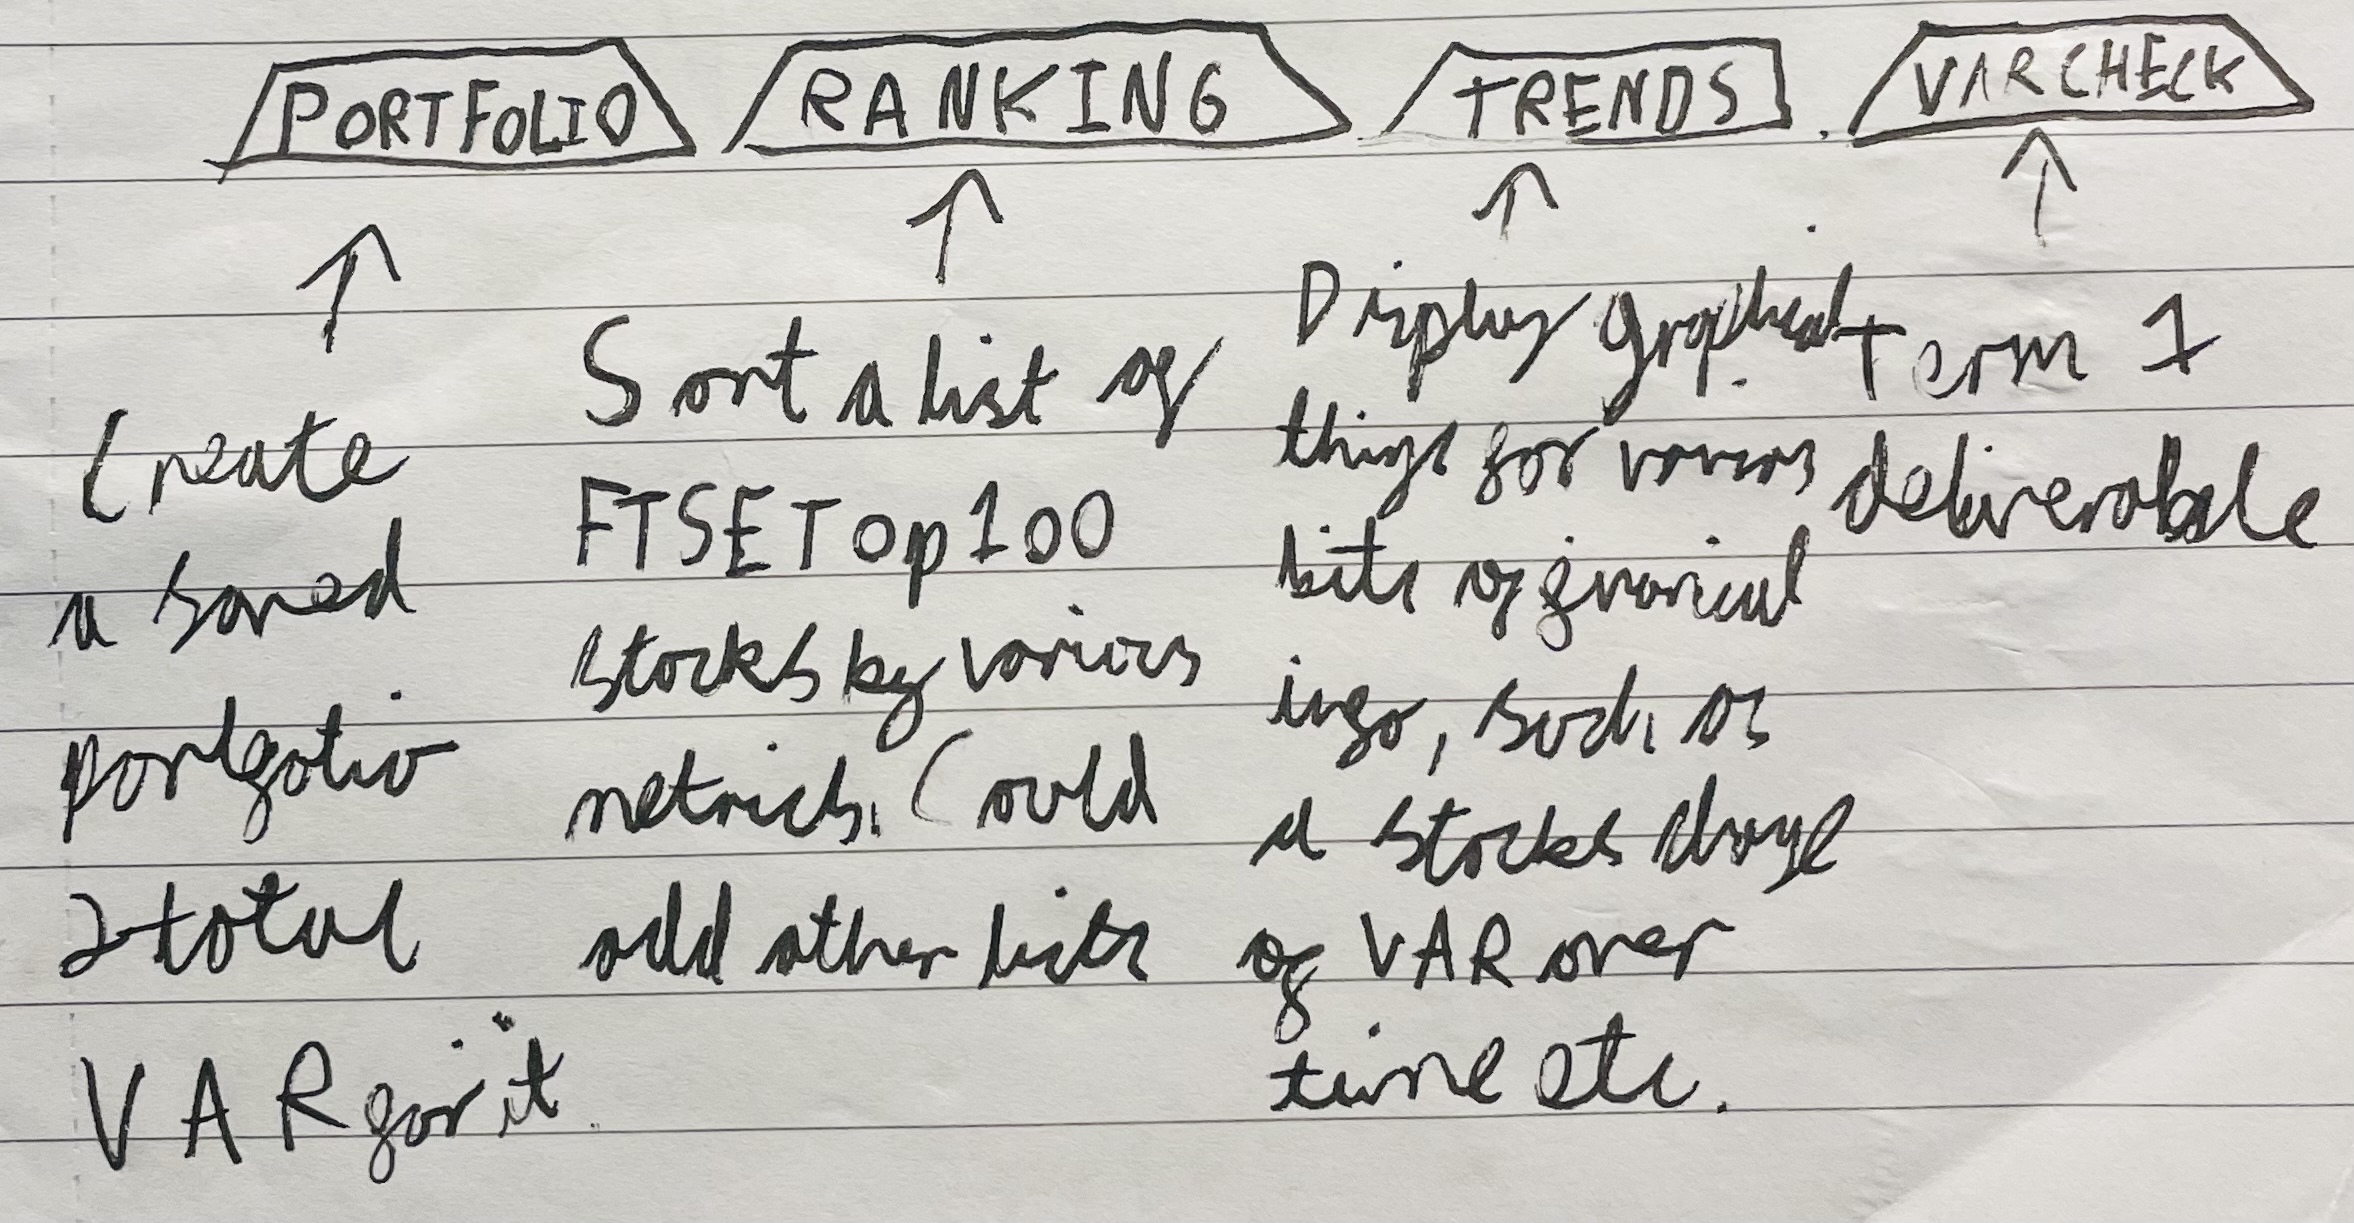
\includegraphics[width=0.7\textwidth]{Images/Term 2 Images/IMG_1346.jpg}
  \caption{Tabbing Conceptualisation for Switching Between Screens}
  \label{fig:Tabbing Concept}
\end{figure}

With this, I came up with the 4 screens that I wanted to implement into my program, those being:
\begin{itemize}
  \item \textbf{Portfolio Screen:} The main screen when you open up the program, where you can create a portfolio, select the stocks and amount of shares that you want for it and generate the Value at Risk for the total value.
  \item \textbf{Rankings Screen:} Have a list of stocks, such as the FTSE100, and be able to rank them based on their VaR values, as well as other metrics, possibly allowing for being able to select different lists.
  \item \textbf{Trends Screen:} Using financial information to display graphical trends for stocks, such as the price of a stock over a period of time, or the VaR of a stock over a period of time.
  \item \textbf{VaRCheck Screen:} A home for my previous initial design deliverable, still practical for what its used for, but not versatile enough to work as an independent program, so it can be used to check theoretical values at risk for the individual FTSE100 stocks.
\end{itemize}

I was inspired by the design of tabs in most modern browsers, which are used to switch back and forth between websites. I also liked the trapezium shape I used, but I knew I would fit the constrains of whatever my program needed to function optimally. With this, I knew that I had to implement it into my program, so I could begin the development of these screens, allowing for the functionality I was aiming for within my final deliverable.\\\vspace{0.3cm}

\subsubsection{Tabbing System and Workspace Structure}
Up until now, I had my whole program within one file, \texttt{Initial Design Test.py}, and the subsequent \texttt{IDT.kv} file alongside it, but for this, I knew that I wanted to be connecting a bunch of screens together, which would be far too much code to have it all handled within one file. So, since I'm' developing this program adhering to Object Oriented principles, I decided to use a hub program, and split up all my other screens into separate files, and then put into specific folders within the same directory as the main program.\\\vspace{0.3cm}

For this I had to seperate my original file into one called \texttt{Final Design.py}, which would be the hub program, and my renaming my old file to be the screen, \texttt{VaRChecker.py}. This involved removing the kivy app definition and running section and putting it in the new program, intialising the app, certain imports and the window size (which had to be increased to be able to fit in the new tabs). The old program was then placed into a folder called \texttt{Screens}, and the new program remained at the base of the previous directory. Following on from this, I created the other 3 screens, \texttt{PortfolioScreen.py}, \texttt{RankingsScreen.py}, and \texttt{TrendsScreen.py}, and placed them in the same folder as the \texttt{VaRChecker.py} file.\\\vspace{0.3cm}

For each of these however, I needed to create the specific .kv file to match, to define the kivy visuals. To do this, I created a folder called \texttt{kvFiles}, and implemented the files \texttt{PortfolioScreen.kv}, \texttt{RankingsScreen.kv}, \texttt{TrendsScreen.kv}, and \texttt{VaRChecker.kv} (which had the same code as \texttt{IDT.kv}). But even with these individual files, my new Final Design file could not see them. To fix this, I created the final new file, \texttt{FD.kv}, within the same directory as my \texttt{Final Design.py}, that I would use to link all the others together, using: \\\vspace{0.3cm}

\begin{verbatim}
  #:include kvFiles\VaRChecker.kv
  #:include kvFiles\Trends.kv
  #:include kvFiles\Portfolio.kv
  #:include kvFiles\Rankings.kv
\end{verbatim}

\vspace{0.3cm}
This would allow all my .kv files to work together, but the same could not be said for the python files, since the main app being run within the final design did not have access to the other screens yet. To implement the communication between the screens to the app, I needed to use: \\\vspace{0.3cm}

\begin{verbatim}
  from kivy.uix.screenmanager import ScreenManager
  from Screens.Portfolio import Portfolio
  from Screens.Rankings import Rankings
  from Screens.Trends import Trends
  from Screens.VaRChecker import VaRChecker

\end{verbatim}

This would give my main program access to the other screens, and subsequently link them all together within the screen manager. To do this, within the initial build method immediately defined within the app, I defined my screen manager, and added all the screens to it as widgets. Now that they were inside my screen manager within the building app, I needed to create the tabs for them to be displayed, this being done by creating a BoxLayout taking up the top 10\% of the screen, that for each screen within the screen manager, would create a named button 25\% of the apps size wide, allowing for the creation of 4 equal sized buttons spanning the top of the screen, with a a bound on\_release function set to a method I created, taking the text instance found on the selected button and switching the screen managers "current screen" to be the screen with the clicked name. This ended up functioning perfectly, I had to create blank kv files that were gray for all the screens that had not been populated yet, but the code and tabs worked great, with it implementing a swipe animation clicking between the screens already implemented (although it would only swipe from left to right, no matter what direction you were swapping between screens). The tabs and code can be seen below:\\\vspace{0.3cm}

\begin{verbatim}
  sm = ScreenManager()        
  sm.add_widget(Portfolio(name='Portfolio'))
  sm.add_widget(Rankings(name='Rankings'))
  sm.add_widget(Trends(name='Trends'))
  sm.add_widget(VaRChecker(name='VaRChecker'))

  def screenSwitch(instance):
      sm.current = instance.text

  tabs = BoxLayout(size_hint=(1, 0.1), pos_hint={'top': 1})
  for screen in sm.screens:
      print(screen.name)
      tabButton = Button(text=screen.name, size_hint=(None, 1), width=200)
      tabButton.bind(on_release=screenSwitch)
      abs.add_widget(tabButton)

  layout = BoxLayout(orientation='vertical')
  layout.add_widget(tabs)
  layout.add_widget(sm)
  return layout
\end{verbatim}

\begin{figure}[h]
  \centering
  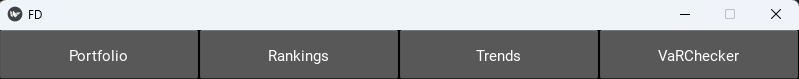
\includegraphics[width=1\textwidth]{Images/Term 2 Images/tabs.png}
  \caption{Tabs Implemented into the Program}
  \label{fig:Tabs}
\end{figure}


\subsection{Developing a Portfolio Screen}
When initially creating portfolio management software, you need to take into account many things, such as:
\begin{itemize}
  \item \textbf{Data Collection}: The software needs to be able to collect all relevant data for a stock and update it's pricing in effective real-time.
  \item \textbf{Data Storage}: You need to consider how and where the data will be stored. This is usually done within a database or in the cloud, but it depends on the software you're utilising.
  \item \textbf{User Interface}: The software should have a user-friendly interface that allows users to easily manage their portfolio and understand the interactions between the options that they are presented with.
  \item \textbf{Performance}: The software should be able to handle large amounts of data being stored and processed, to perform calculations quickly enough for the user experience to not be affected.
  \item \textbf{Scalability}: The software should be able to handle an increasing number of stock data, and it should be able to handle multiple users if being user in different environments.
\end{itemize}

These in tandem will all help when creating this form of software, and help when visualising how you want the software to look and act. For this, I once again drafted an initial design, which I will explain in parts below:\\\vspace{0.3cm}

\begin{figure}[h]
  \centering
  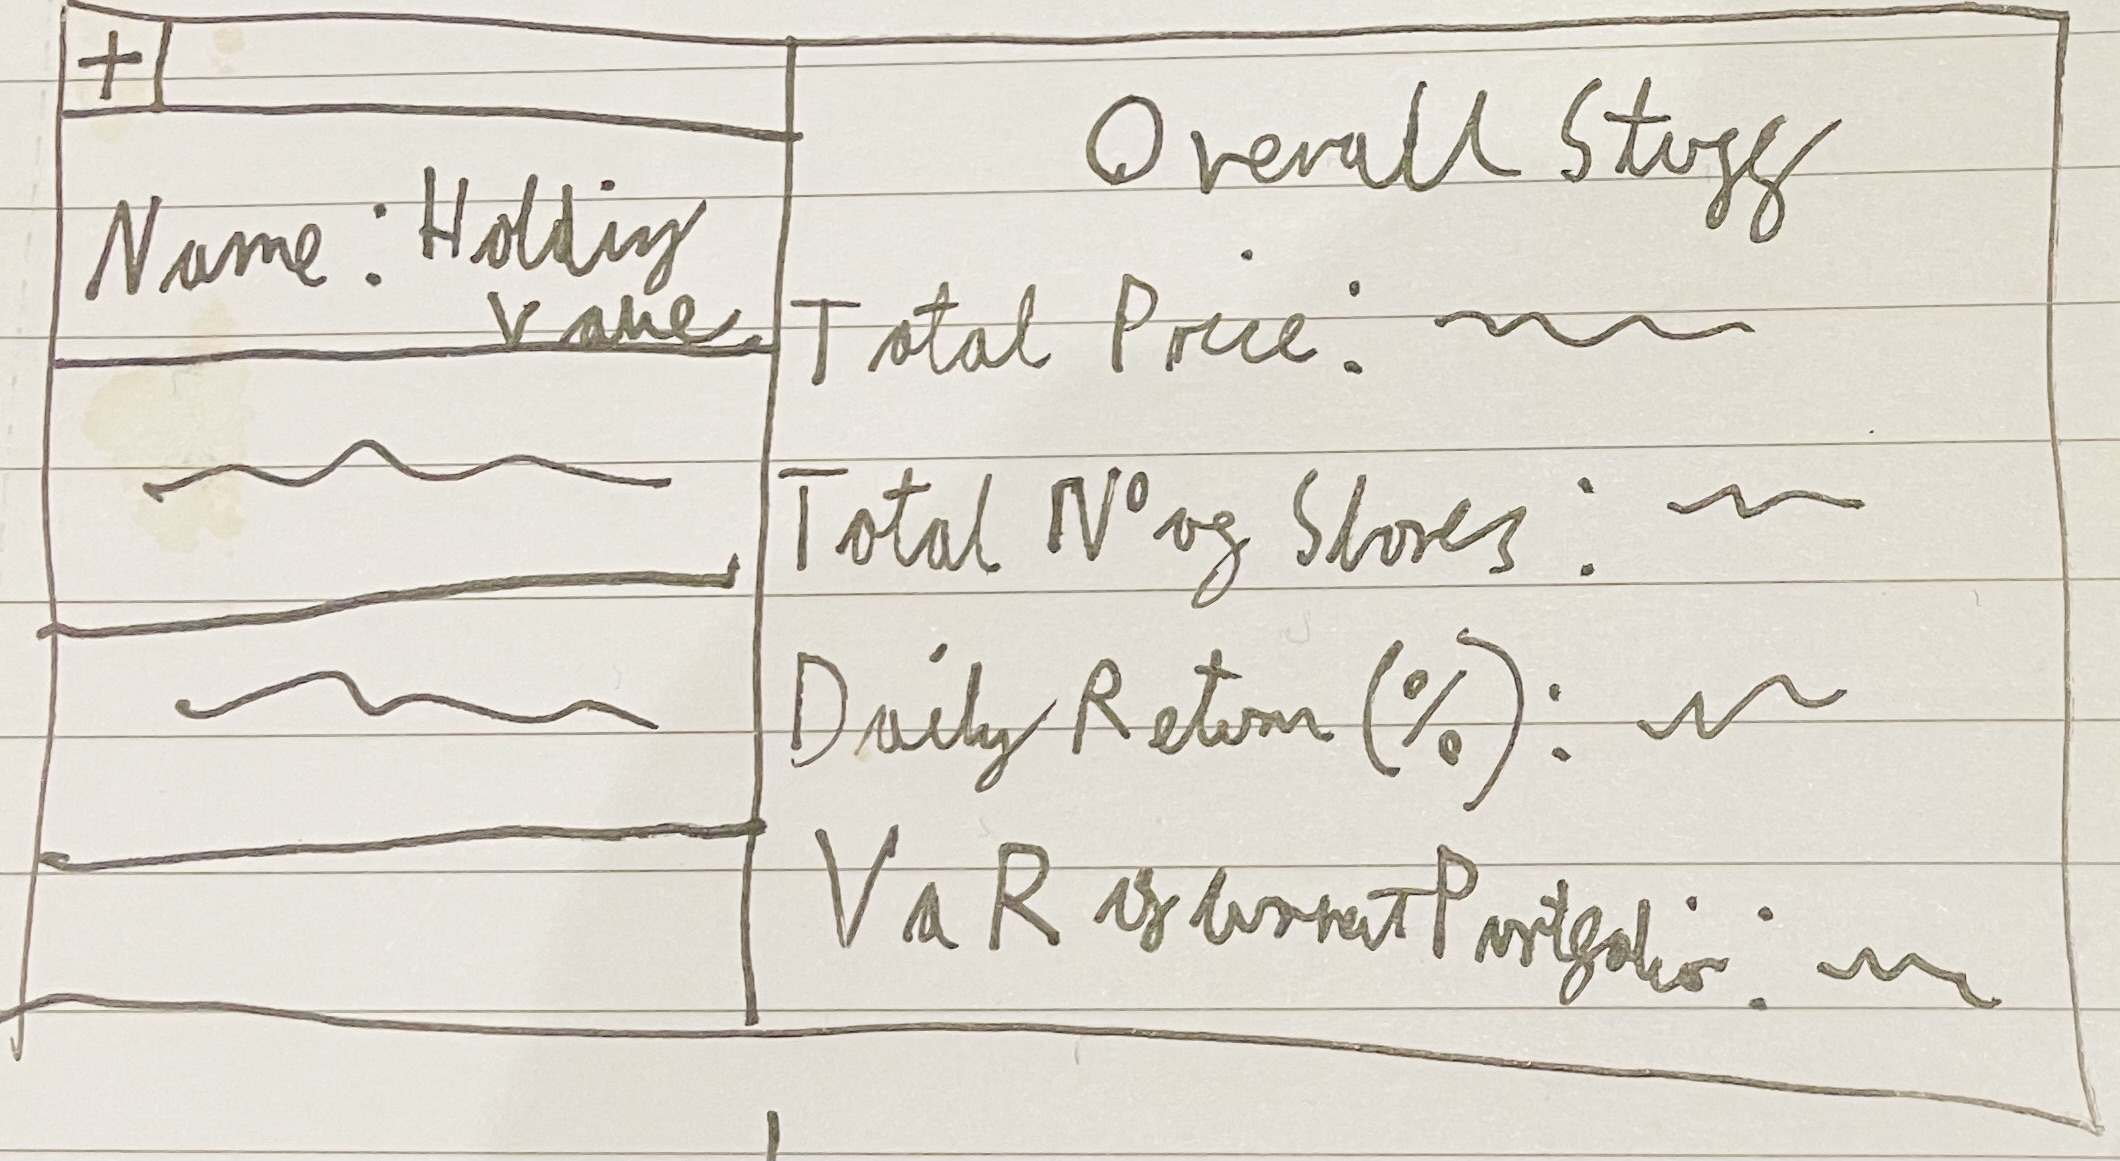
\includegraphics[width=0.7\textwidth]{Images/Term 2 Images/IMG_1117.jpg}
  \caption{Draft Portfolio Screen - Top}
  \label{fig:Portfolio Screen Draft Top}
\end{figure}

\begin{figure}[h]
  \centering
  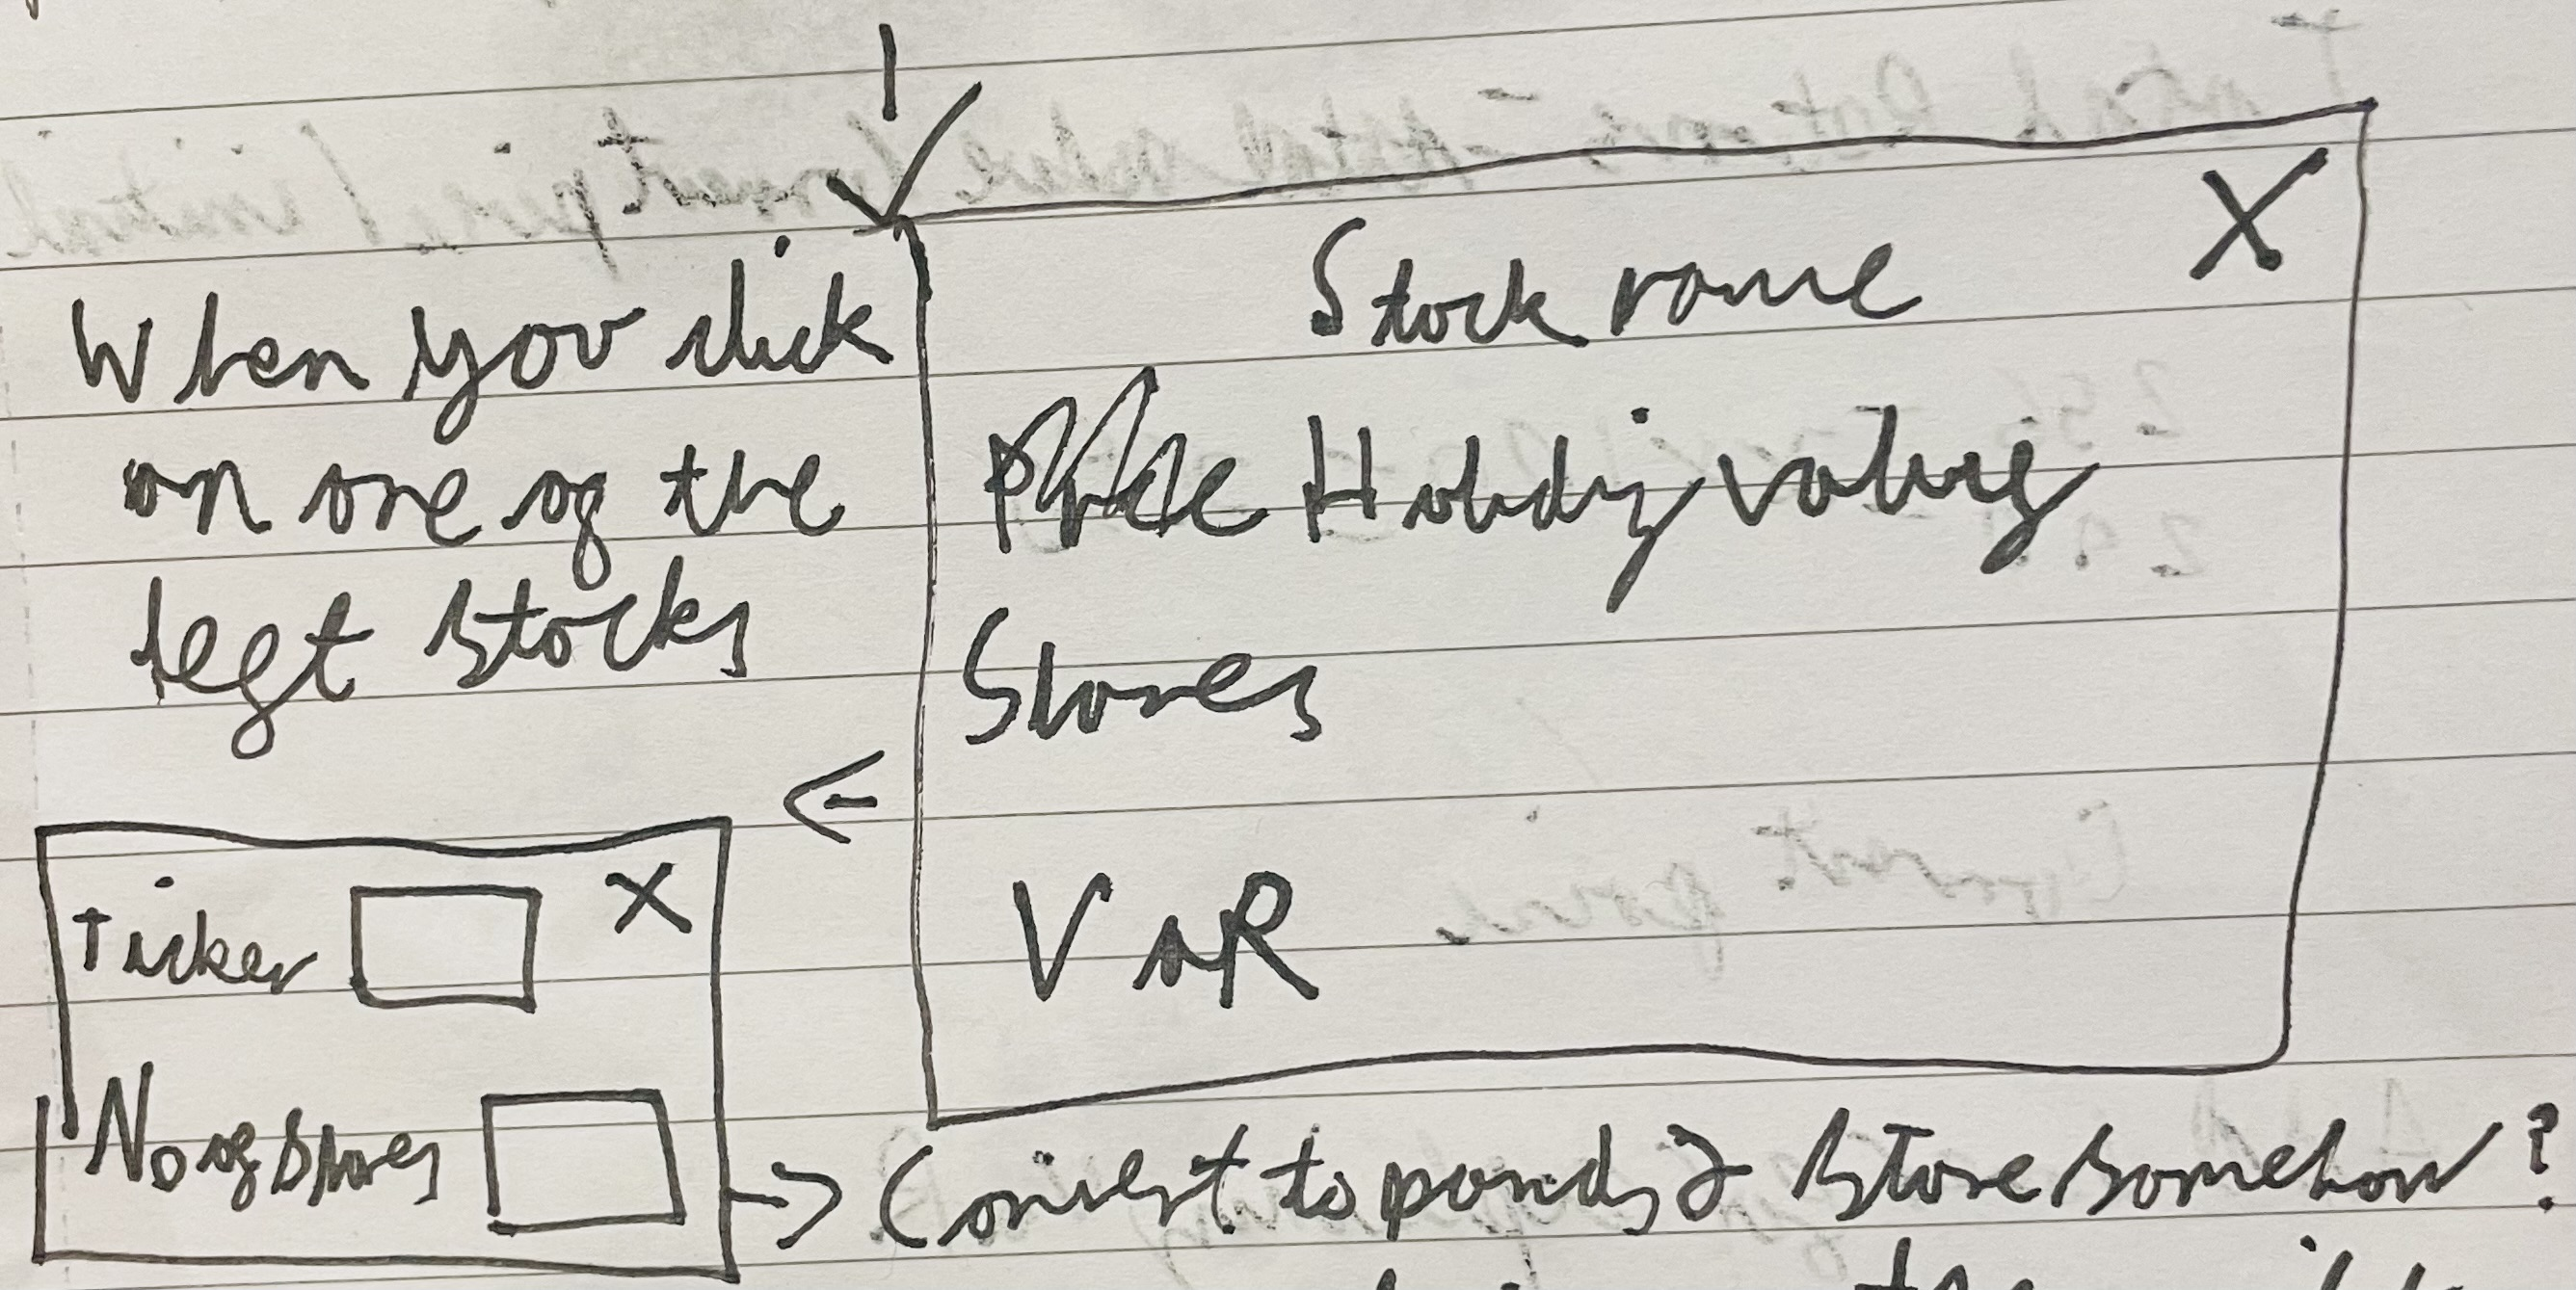
\includegraphics[width=0.7\textwidth]{Images/Term 2 Images/IMG_1347.jpg}
  \caption{Draft Portfolio Screen - Bottom}
  \label{fig:Portfolio Screen Draft Bottom}
\end{figure}

In figure \ref{fig:Portfolio Screen Draft Top}, my plan is to create a portfolio system where you can store your stock within a scrolling list on the left hand side. This is the same concept I used for my initial design, within my VaRChecker screen now, but you can add and remove stocks from this dynamic list. To add the stocks, you would click on the button in the top left, which would create a pop-up window, a feature that I did not utilise within my initial design, but upon further use of the kivy documentation [\ref{ref13}] I discovered its existence and apparent usefulness for a situation like this. On the right hand side, it would display the overall total price/value of the portfolio, being calculated by getting the live prices of stocks, multiplied by the number of stored shares for each stock. It would also display the number of stocks (a rather useless metric from a financial standpoint but a nice feature to have), the daily return of the portfolio, and the Value at Risk of the portfolio, which would be calculated using the Monte Carlo Simulation method I had previously implemented. It is also noted that I want the stocks on the left to have their name displayed, as well as their holding value, since it can be used to compare to the overall value on the right, since both would be shown at the same time.\\\vspace{0.3cm}

For figure \ref{fig:Portfolio Screen Draft Bottom}, I wanted to have it so when you select one of the stocks on the right, it replaces the overall portfolio stats on the right with specific ones for the currently selected stock, such as its name, holding value, No. of shares (much more important for this context), and individual VaR. This would allow for a more in-depth analysis of individual stocks within the portfolio, and allow for a more detailed understanding of the risks and rewards of each stock whilst still seeing how diversification affects the stability of Value at Risk. It would have a cross in the top right, allowing you return to your overall view of the portfolio. I also created a small sketch for how I would want the pop-up to look, having to inputs for ticker (since this is how yfinance would download it) and no's of shares, as well as a button to exit the pop-up, resulting in the end of the interaction.\\\vspace{0.3cm}

With these initial ideas in place, I set to work on implementing them. Since this was a large program, with many different computational elements and visual designs within both the files used, I will attempt to showcase key points of its development with accompanying visual aid when possible, but since it cannot cover everything, the full code can be found in the appendix.\\\vspace{0.3cm}

\subsubsection{Initial Structure and Pop-Up}
My original structure for the file consisted of 3 classes, these being the screen class \texttt{{Portfolio}}, the one being referenced within my main hub, the button class \texttt{Stocks}, where I can display the current stocks that my system deals with and can be pressed, and a pop-up class \texttt{InputStock}, a way for me to add those stocks to the system. You would use a button in the top left to access the pop-up, which would create and store stock information. Since I wanted the stocks to be retained after you had closed and reopened the application, I had different options available to me to consider, due to the vast amount of imports and libraries that Python can utilise to store data, such as database frameworks, even using a notepad file, etc.\\\vspace{0.3cm}
But once again, within the kivy documentation [\ref{ref13}], there's a built in way to easily store data within a JSON file in the directory your program is running in, using the module \texttt{kivy.storage.jsonstore}. It uses an easy dictionary format with a key, and can store all the relevant stock information I would need. When the pop-up is successfully dismissed, it will call a function within \texttt{Portfolio} to run an update on the stocks list, checking the JSON file and adding all of them as widgets into a scrollable list, with each stock element containing the current stock being displayed's data, which can be referenced when it's selected later to have its information displayed specifically on the right hand side. Below are the respective sections generally described above: \\\vspace{0.3cm}

\begin{verbatim}def openPopup(self):
  popup = InputStock()
  popup.bind(on_dismiss=self.loadStocks)
  popup.open()
\end{verbatim}

\vspace{0.3cm}
This creates an instance of my pop-up class, binds the \texttt{on\_dismiss} function to the loadStocks method, and then opens the pop-up.\\\vspace{0.3cm}

\begin{verbatim}
  from kivy.storage.jsonstore import JsonStore
  ...
  class InputStock(Popup):
      def __init__(self, **kwargs):
          super().__init__(**kwargs)
          self.size_hint = (0.5, 0.5)
          self.title = 'New Holding'

      def saveStock(self):
          stockData = {
              'ticker': self.inputTicker.text,
              'overallShares': self.inputShares.text,
          }
          JsonStore('holdings.json').put(stockData['ticker'], **stockData)
          self.dismiss()
\end{verbatim}

\vspace{0.3cm}
At the top of the file I import the JsonStore module, and then create my pop-up class, setting its size and title. The saveStock method is called when the save button is pressed, defined within the \texttt{.kv} file, creating a dictionary of the inputted stock data and storing it in the JSON file, then finally dismissing itself. The resulting stored data, for one of my initial uses when using my "holdings", looks like this - \texttt{\{"test ": \{"ticker": "test ", "overallShares": "test"\}\}}\\\vspace{0.3cm}

\begin{verbatim}
  def loadStocks(self, *args):
      store = JsonStore('holdings.json')
      self.ids.stockCards.clear_widgets()

      for stockKeys in store:
          stockData = store.get(stockKeys)
          self.addStock(stockData)
\end{verbatim}

\vspace{0.3cm}
Upon dismiss, the \texttt{loadStocks} method is called, which opens the JSON file, clears the current stock list to make sure duplicates are not created, and iterates over all the keys in the JSON file, adding each stock to the list of stocks using my addStock function, that passes the relevant data into the stocks class.\\\vspace{0.3cm}

\begin{verbatim}
  class Stocks(Button):
        self.stockInfo = {
            'ticker': ticker,
            'overallShares': overallShares,
        }
\end{verbatim}

\vspace{0.3cm}
Within the class, I create a dictionary to store the stock information, so it can be later referenced when the stock is selected. This allowed me to store and accumulate stocks, that I could visually see added to my screen, but I did not have any deleting process implemented, so I would have to delete them by manually deleting them within the JSON for now. I also set it so that I had default values displayed on the stock information section, and utilised the neutral colour scheme for what I could with the presentation, sticking to colours the I felt were inoffensive from my VaRChecker's style. This resulted in figure \ref{fig:Early Portfolio}, very basic but apparent how the screen will be developed from now on. \\\vspace{0.3cm}

\begin{figure}[h]
  \centering
  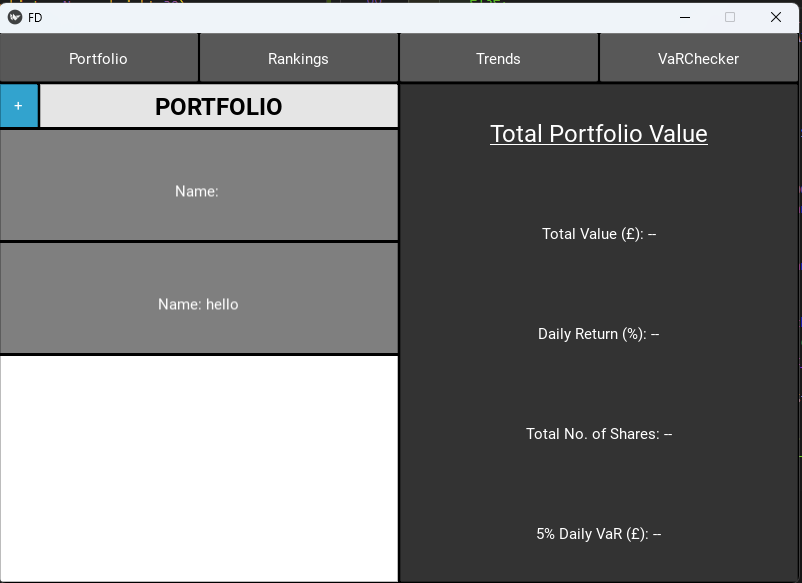
\includegraphics[width=0.7\textwidth]{Images/Term 2 Images/image (16).png}
  \caption{Early Portfolio}
  \label{fig:Early Portfolio}
\end{figure}

\subsubsection{Storing Stocks and Calculating Portfolio Value}
At this point in my projects development cycle, I realised that the nuance between my Rankings Tab and my Trends tab were irrespective for what I needed to create and what I could deliver. Because of this, I realised I could integrate both into each other, graphically display whatever ranking I may compute within its own section, that also would show the trends that my stocks were taking. This resulted in me removing the Rankings tab and planning to just create the Trends tab, which can be seen at the top of the program in figures going forward.\\\vspace{0.3cm}

Since I had not implemented verification, I had to be certain that the tickers I entered into my pop-up were correct, and if so, yfinance would be able to correctly download the data. This is crucial, since I would need to retrieve and store the initial stock price of the data as soon as I added it to my stocks list, since it would be needed to refer upon in the future to compare to whatever the continued current price would be going forward, needed when calculating return. To do this I used:\\\vspace{0.3cm}

\begin{verbatim}
  initialPrice = yf.download([self.inputTicker.text], period='1d')
                                         .tail(1)['Close'].iloc[0]
\end{verbatim}

\vspace{0.3cm}
Which would download the stock price for the last day, and then take the last value in the list, which would be the current price of the stock. Previously, using yfinance's \texttt{.info['regularMarketPrice']} command would have been a viable way for me to retrieve the current price easily, but due to certain limitations that Yahoo's financial API had put into place recently, I was unable to use this method, and had to find this work around, which I continue to use going forward since it presents the same results. This initial price would be stored within the JSON to be referenced later.\\\vspace{0.3cm}

With this initial price now stored, I could now calculate the majority of the necessary information that my program would need to consistently display within my totals section. This would be done (once checking that the length of the JSON is not 0) by iterating over all the stocks in the JSON file, and for each stock, downloading its current price, calculating it's total value by multiplying it with the stored shares quantity, summing these all together, resulting in the Portfolio's current total value. The total shares would be added up within the iteration, and the daily return I adapted into just being the total return of the portfolio, a percentage based on all the current prices together being compared to all of the initial prices summed together.\\\vspace{0.3cm}

\begin{verbatim}
  def initialStockTotals(self, *args):
      store = JsonStore('holdings.json')
      if len(store) != 0:
          totalValue = 0
          ...
          totalShares = 0

          for stockKeys in store:
              stockData = store.get(stockKeys)
              currentPrice = yf.download([stockData['ticker']], period='1d')
                                                   .tail(1)['Close'].iloc[0]

              totalValue = totalValue + (currentPrice * float(stockData['sharesOwned']))
              totalCurrentPrices = totalCurrentPrices + currentPrice
              totalInitialPrices = totalInitialPrices + float(stockData['initialPrice'])
              totalShares = totalShares + int(stockData['sharesOwned'])
          totalReturn = ((totalCurrentPrices / totalInitialPrices) - 1) * 100

          self.stockName.text = "[u]Total Portfolio Value[/u]"
          self.totalValue.text = "Total Value: £{:,.2f}".format(totalValue)
          self.totalReturn.text = "Total Return: {:.2f}%".format(totalReturn)
          self.totalShares.text = f"Total No. of Shares: {totalShares}"
\end{verbatim}

\vspace{0.3cm}
At the end, it changes the references to the id's in the \texttt{.kv} file's text to be the computed value, displaying them on the right hand side. This method would be called upon when the program is being initialised, and upon the dismissal of the pop-up, to ensure that the totals are always up to date.\\\vspace{0.3cm}

\subsubsection{Background App Refresh and Race Conditions}
But I want to have it so that the program can update the stock prices in real-time, so that the user can see the changes in their portfolio as they happen. Whilst realtime is a bit of an impossibility using python, since the download isn't instant and gets worse with more stocks being stored, having it re-download all stocks every 60 seconds seems a lot more reasonable, especially since stocks don't change in value that quickly. Within my time to decide to do this, I had implemented a \texttt{specificStockTotals} method that would be called upon when a stock was selected, and would display the specific stock's information on the right hand side, with generally the same logic as the previous section. Since I would still want this data to be updated every minute when a stock is selected, as well as when the portfolio totals are being displayed, I decided to utilise Kivy's Clock functionality.\\\vspace{0.3cm}

By using \texttt{Clock.schedule\_interval()}, a function found within the \texttt{kivy.clock} module, I was able to call a function every 60 seconds, which would be my \texttt{initialStockTotals} method, which would update the stock prices and the portfolio totals. I also had a subsequent one within my \texttt{specificStockTotals} method that would do the same thing when a specific stock was selected. But this could result in the program trying to update and download the stock prices at the same time, since only downloading one stock when all are necessary would crash the program. To ensure that one clock was being run at one time (preventing any race conditions) and that the clock was not calling an instance inside itself recursively (resulting in it never being able to be stopped), I utilised the code below: \\\vspace{0.3cm}

\begin{verbatim}
  def specificStockTotals(self, *args):
      if isinstance(self.iSTCheck, ClockEvent):
          Clock.unschedule(self.iSTCheck)
          self.iSTCheck = None

      if not isinstance(self.sSTCheck, ClockEvent):
          self.sSTCheck = Clock.schedule_interval(self.specificStockTotals, 60)
\end{verbatim}

\vspace{0.3cm}
Using stored checker methods that were initialised during the classes startup, it would check if the other clock was already running, and if so, unschedule it, and then schedule this new clock. This would ensure that only one clock was running at one time, and that the clock was not calling itself recursively, allowing for the program to update the stock prices every 60 seconds completely dependant on what they had selected at the time.\\vspace{0.3cm}

\subsubsection{Value at Risk Calculators}
You may have noticed that when creating the displays for the total and specific stocks, that I had not displayed or generated the Value at Risk to be displayed for either. This was because I had not yet implemented the Monte Carlo Simulation method into the program, and I would need to do so to be able to calculate the VaR for the portfolio. I had tested single stock calculations for VaR with this method as well, but it did not work, so I decided that I would just use my Model Simulation (Variance-Covariance) method for the single stock VaR calculations, and the Monte Carlo Simulation for the portfolio VaR calculations, as I have had both working in other programs/screens. I chose to use model over historical simulation as when back-testing, the resultant p-value were much higher/more consistent when using the model method, so I believed it to be more reliable. To implement these methods, I decided to create another class (all subsequent new classes mention all being within this same \texttt{Portfolio.py} file.) called \texttt{VaRCalculators}, that would contain all the methods needed to calculate the VaR for the portfolio and the individual stocks. An instance of this would then be created when the screen was initialised (\texttt{self.varCalc = VaRCalculators()}), and the methods within could be referenced  whenever needed in the stock total clock cycles.\\\vspace{0.3cm}

\begin{verbatim}
  class VaRCalculators:
    def __init__(self, *args):
        self.rlPercent = 0.05
        self.timeHori = 1

    def modelSim(self, totalValue, stocks):
        closeDiffs = stocks['Close'].pct_change().dropna()
        return "{:,.2f}".format((-totalValue*norm.ppf(self.rlPercent/100,
        np.mean(closeDiffs), np.std(closeDiffs)))*np.sqrt(self.timeHori))
\end{verbatim}

\vspace{0.3cm}
The \texttt{VaRCalculators} class is initialised with the risk level percentage and the time horizon, and the \texttt{modelSim} method is used to calculate the VaR for the single selected stock. It takes in the current value of the stock (being the current price times the shares owned) and the downloaded stock data, necessary for calculating the daily returns, and then uses the  Model Simulation seen in section \ref{Command Model}, which is then returned. This method would be called inside the specific stock cycle, and return the VaR to be displayed, rounded to two decimal places and with comma formatting.\\\vspace{0.3cm}

For the total portfolio calculations however, I needed to implement the Monte Carlo method, as well as calculate the weightings of all the stocks. But since I had already implemented these kind of calculations in a previous section and had passed in all the stock information, I would use the same logic to calculate weightings and run my subsequent simulation.\\\vspace{0.3cm}

\begin{verbatim}
  def monteCarloSim(self, totalValue, stocks):
      weightings = np.zeros(len(stocks['Close'].columns))
      for x, stockKey in enumerate(store):
          stockData = store.get(stockKey)
          currentPrice = stocks['Close'][stockData['ticker']]
          .loc[stocks['Close'][stockData['ticker']].last_valid_index()]

          currentValue = currentPrice * float(stockData['sharesOwned'])
          weightings[x] = currentValue / totalValue
  
      closeDiffs = stocks['Close'].pct_change(fill_method=None).dropna()
      simNum = 100000
      portfoReturns = np.zeros(simNum)
  
      optimisedSim = np.random.multivariate_normal(closeDiffs.mean() 
                         ,closeDiffs.cov(), (self.timeHori, simNum)) 

      for x in range(simNum): 
          portfoReturns[x] = np.sum(np.sum(optimisedSim[:, x, :] 
                                          * weightings, axis=1))
          
      return "{:,.2f}".format(-np.percentile(sorted(portfoReturns), 100 
                                          * self.rlPercent)*totalValue)
\end{verbatim}

\vspace{0.3cm}
This new version of my Monte Carlo Simulation would calculate the weightings of all the stocks by iterating over all the stocks in the JSON file, using this to access each index within the downloaded stock data, calculating the current value of the stock, and then dividing it by the total value of the portfolio. It would then calculate their daily returns, and run the simulation 100,000 times. However, I realised that numpy had a built in way to perform the simulation by utilising how \texttt{np.random.multivariate\_normal()} works. By defining the final section within it with both \texttt{(self.timeHori, simNum)}, it would allow me to create a 3D array of the simulations, providing me with the data I needed in one statment. I still needed to run all the simulations, so I created a for loop that would multiply the optimised simulation by the weightings, summing them all together along the outer axis, and then summing them all together again, we result in finally obtaining the portfolio returns. This method ends up being a lot more efficient than my previous method, saving a lot of loading time for the application, which is crucial for the user experience when navigating a the main portfolio screen. Finally, the VaR is calculated by taking the 5th percentile of the sorted returns, and then multiplying it by the total portfolio value, returned correctly formatted.\\\vspace{0.3cm}

\subsubsection{Finding Comparny Names and Back Button}
As I was developing the program, there was a lot of visual iterations and changes to formatting and presentation that I can't cover in this report, but one of the features I knew I would need to have would be the actual display of the full company name, since trying to remember what each company was based on tickers in a stock list felt terrible, this being seen in figure \ref{fig:Ticker Names} (you can also see the reduced tabs at the top). Usually, this could have been done once again using the slightly altered aforementioned yfinance \texttt{.info['name']} method, but this was still broken, so I had to come up with a more creative solution.\\\vspace{0.3cm}

\begin{figure}[h]
  \centering
  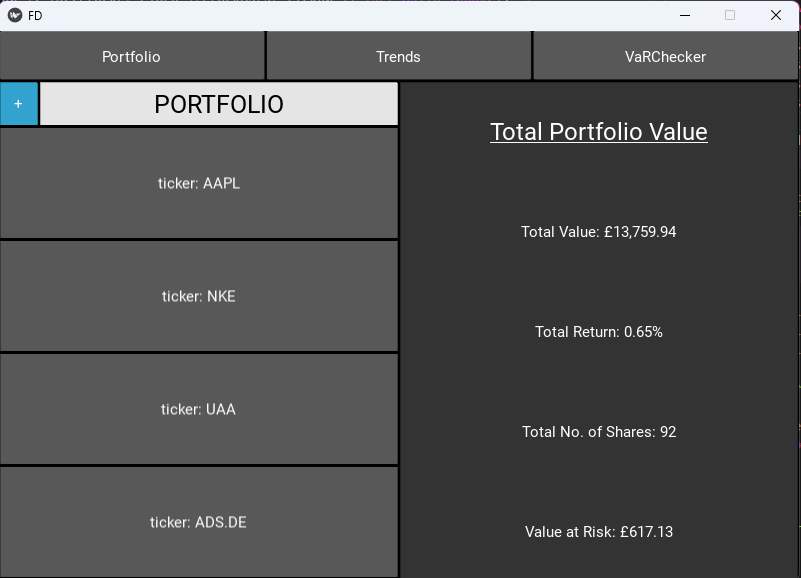
\includegraphics[width=0.7\textwidth]{Images/Term 2 Images/image (15).png}
  \caption{Ticker as Stock Names}
  \label{fig:Ticker Names}
\end{figure}

Yahoo finance has a fantastic website system for displaying their stocks, where every single stock page you find is located at: \url{https://uk.finance.yahoo.com/quote/}\texttt{XXXX}, where \texttt{XXXX} is the ticker of the stock you are querying. And on each one of their pages, towards the top you will always find the full company name displayed next to its ticker. Upon using inspect element on this section (a feature of most modern browsers allowing the user to see the underlying HTML of a webpage), I could see this \texttt{h1} element was always created using the same class, \texttt{D(ib) Fz(18px)}.\\\vspace{0.3cm}

\begin{figure}[h]
  \centering
  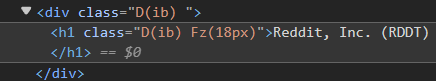
\includegraphics[width=0.7\textwidth]{Images/Term 2 Images/HTML Element.png}
  \caption{Ticker as Stock Names}
  \label{fig:Ticker Names}
\end{figure}

\vspace{0.3cm}
With this knowledge, I knew that I had to find a way to obtain the html of these pages I can query, with just the information given by a stock ticker. For retrieving the page, I could use the python \texttt{requests} module to download the html of a webpage, but for the parsing of the html, I would need to use \texttt{BeautifulSoup}. This module allows for the parsing of html and xml documents, and can be used to extract information from them, such as the text within the element that I needed to find.

\begin{verbatim}
  def findCompanyName(self, ticker):
      yFinancePage = f"https://finance.yahoo.com/quote/{ticker}"
      headers = {
      'User-Agent': 'Mozilla/5.0 (Windows NT 10.0; Win64; x64) AppleWebKit/537.36 
      (KHTML, like Gecko) Chrome/123.0.0.0 Safari/537.36 Edg/123.0.0.0'
      } 

      response = requests.get(yFinancePage, headers=headers)
      soup = BeautifulSoup(response.content, 'html.parser')
      companyName = soup.find('h1', class_='D(ib) Fz(18px)')

      return companyName.text
\end{verbatim}

\vspace{0.3cm}
This method would take in a ticker, concatenate it with a url to create the link for my needed stock page, and then download the html of the page using the requests module. Whilst this method would work for most of the stocks that I tried for, any that had "Non-US" denoters (stocks that aren't listed on NASDAQ, instead with London Stock Exchange with .L or country specific Germany with .DE) would fail to have their page load and stored correctly. To combat this, I would employ the use of a User Agent, found at \url{https://user-agents.net/my-user-agent}, within the headers of the request, which would simulate the request to appear as if it was coming from a browser, and not a python script, successfully allowing me to download the HTML data.\\\vspace{0.3cm}

I would then proceed to parse the html using BeautifulSoup, and find the \texttt{h1} element with the class I needed, and return the text within it, which would be the full company name. This method would now be called upon whenever a stock was added to the list, storing the full company name along with ticker inside the JSON file, and with a small adjustment to stocks, promptly displayed in tandem on the stock list, as seen in \ref{fig:Stock and Ticker Names}. This would allow for a much more user-friendly experience when navigating my app, I'm aware that it would be optimal to use a stock name when adding it to your portfolio but I could not envision this capability working vice versa due to the nature of the URL's that Yahoo Finance provides, since it is through that I can use the ticker and find the stock names in the first place.\\\vspace{0.3cm} 

The new resultant holding information would look like this - \texttt{\{"ADS.DE": \{"name": "adidas AG (ADS.DE)", "ticker": "ADS.DE", "sharesOwned": "50", "initialPrice": 201.39999389648438\}\}}\\\vspace{0.3cm}

\begin{figure}[h]
  \centering
  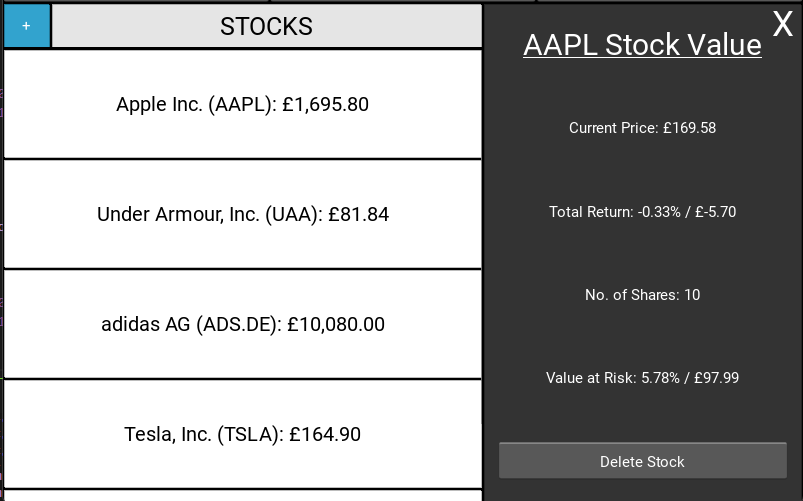
\includegraphics[width=0.7\textwidth]{Images/Term 2 Images/image (12).png}
  \caption{Stocks List with Company Names}
  \label{fig:Stock and Ticker Names}
\end{figure}

\vspace{0.3cm}
Another thing to note within the figure \ref{fig:Stock and Ticker Names} is the addition of a back button, which can be seen in the top right. I assumed with the \texttt{+} symbol for adding a stock and this \texttt{X} button, that the user would intuitively understand what each were trying to represent, since it adheres to the genreal design principles found within the creation of graphical interface. (IDK ADD A REFERENCE HERE TO UCD MAYBE). On the Total Portfolio display, the back button can still be seen in the same place, but with its opacity and ability to be pressed set to 0. When you run the \texttt{specificStockTotals} method, it would set the opacity to 1 and the ability to be pressed to 1, allowing for the user to return to the total portfolio view. And the code it runs when pressed is simply just \texttt{initialStockTotals()}, redrawing back over it and setting itself to invisible \& untouchable again.\\\vspace{0.3cm}

\subsubsection{Improving Monte Carlo Simulation}
Every time I would switch between my two Portfolio views, it would have to recalculate the VaR, thus running more Monte Carlo Simulations, and slightly lagging the app consistently. Whilst this method was efficient, I wanted to adapt is so that it didn't have to run through all the simulations extensively every time (since the more simulations produced more accurate results that I wanted to have displayed), resulting in me considering the use of a convergence point/threshold. With this, my method would continuously perform simulation steps, incrementing and producing a new VaR result every time, but performing many less simulations to begin with. And as soon as one of these simulations is within the same threshold (1\%) as the last one, I could assume that this was a reasonably accurate estimation of the VaR, returning the latest value for it.\\\vspace{0.3cm}

\begin{verbatim}
  def monteCarloSim(self, totalValue, stocks):
      ...
      simNum = 5000
      convThreshold = 0.005
      previousVar = float('inf')
      converged = False

      while not converged and simNum <= 100000:            
          ...
          currentVar = -np.percentile(sorted(portfoReturns), 100 * self.rlPercent)

          if previousVar != float('inf') and abs((currentVar - previousVar) / 
                                                previousVar) < convThreshold:
              converged = True
          else:
              previousVar = currentVar
              simNum += 50004
\end{verbatim}

\vspace{0.3cm}
I would set the starting simulation number to 5000, the threshold to 0.5\% as it seemed to produce the best results with the speed the VaR would now be calculated at. Upon running the simulation, it would verify that the previous VaR was not infinity, and check if the current VaR was within the threshold of the previous one. If so, it would set the converged boolean to true and return this as the new VaR, and if not, it would set the previous VaR to the current one, increment the simulation number by 5000, and run the simulation again, until it either converges or reaches the point where it is performing 100,000 simulations again. With this convergence method, I was able to obtain the VaR results at a much faster speed, helping improve the app further. \\\vspace{0.3cm}

\subsubsection{Deleting Stocks}
As can also be seen in figure \ref{fig:Stock and Ticker Names}, this time in the bottom right corner, I had implemented a delete button. This would only be visible when a user has selected a stock, since this indicates that the selected stock is the one that can be deleted. Since I found it so useful in creating its own formatted separate section to acquire information, I wanted to use another pop-up to confirm the deletion of a stock, since being able to do it with just one button press would be too much of a risk, especially when dealing with these assets. To do this, I would create a new class for the pop-up in my \texttt{Portfolio.py} file, as well as the subsequent one in my \texttt{Portfolio.kv} file, which I would be able to use to define the pop-ups layout, containing a title, warning and two buttons to press.\\\vspace{0.3cm}

\begin{verbatim}
  <ConfirmDelete>:
      size_hint: 0.5, 0.35
      title: 'Confirm Deletion'
      BoxLayout:
          orientation: 'vertical'
          spacing: 10
          Label:
              text: "Are you sure you want to delete this stock?\n\nIt will be permanent."
              halign: 'center'
              valign: 'center'
          BoxLayout:
              size_hint_y: None
              height: '50sp'
              Button:
                  text: "Yes"
                  on_release: root.on_confirm()
              Button:
                  text: "No"
                  on_release: root.dismiss()
\end{verbatim}

\vspace{0.3cm}
In the process of formatting and changing the functionality of my add stocks pop-up, I discovered that by default, when you click off the pop-up, it would dismiss itself, which was the perfect behaviors for that pop-up, and could be well utilised here again, even if it does also have a no button that will accomplish the same thing. The on\_confirm using the Yes button would send a signal to the root class, but since the button for the pop-up is found within my portfolio class, I had assigned the current ticker to it, so that when it is pressed, the ticker is passed in with it.

\begin{verbatim}
  class ConfirmDelete(Popup):
    def __init__(self, portfolio, ticker=None,  **kwargs):
        super().__init__(**kwargs)
        self.ticker = ticker
        self.currentPortfolio = portfolio

    def on_confirm(self):
        JsonStore('holdings.json').delete(self.ticker)
        self.currentPortfolio.initialStockTotals()
        self.dismiss()
\end{verbatim}

\vspace{0.3cm}
With the ticker being initialised and the current instance of my portfolio class also being passed in, the on\_confirm method can find the ticker within my JSON file, delete it, and call the initialStockTotals method to update the stock list, and then dismiss itself. This would now remove the stock, whenever any of the Stock Totals methods are ran, they also call the \texttt{loadStocks} method, which would update the stock list, removing the deleted stock from the list. This happens dynamically within the list in kivy, so if you're scrolled down within the list when viewing and deleting a stock, it will keep you in the same position you were, not having to scroll back down to find where you were. The pop-up for this can be found below, as well as the portfolio screen display after deleting a stock. \\\vspace{0.3cm}

\begin{figure}[h]
  \centering
  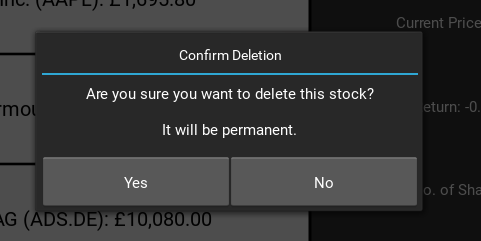
\includegraphics[width=0.7\textwidth]{Images/Term 2 Images/image (10).png}
  \caption{Delete Stock Pop-Up}
  \label{fig:Delete Stock}
\end{figure}

\begin{figure}[h]
  \centering
  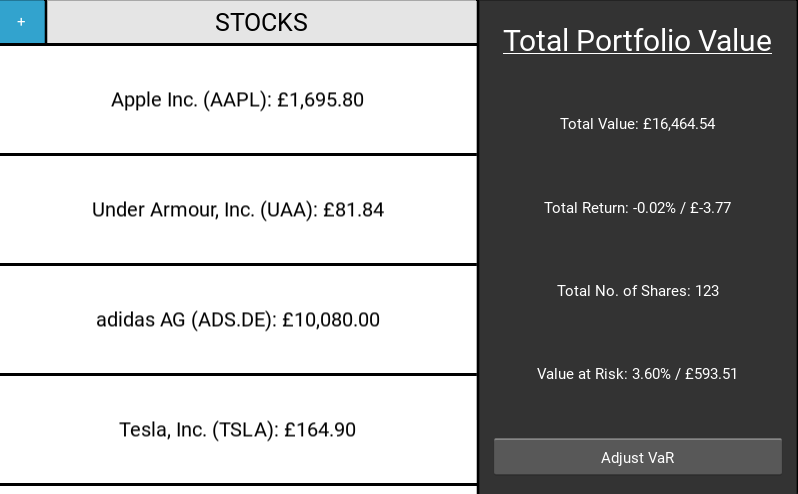
\includegraphics[width=0.7\textwidth]{Images/Term 2 Images/image (13).png}
  \caption{Stocks List after Deleting a Stock}
  \label{fig:Deleted Stocks List}
\end{figure}

\subsubsection{Adjusting VaR Parameters}
As seen in figure \ref{fig:Deleted Stocks List}, in the exact place where the \texttt(Delete Stock) button was, there's another button called \texttt{Adjust VaR}. This is actually the same button but having the text within it changed based on the Portfolio or Specific stock view being used, the logic for which being in a function that checks what text is currently being used by the button to indicate what to do for it. In this instance, it is now used to open up a final pop-up, one used to help explain VaR and add the ability to adjust the parameters of the VaR calculation. My initial creation of it can be seen in figure \ref{fig:OG Adjust VaR}.\\\vspace{0.3cm}

\begin{figure}[h]
  \centering
  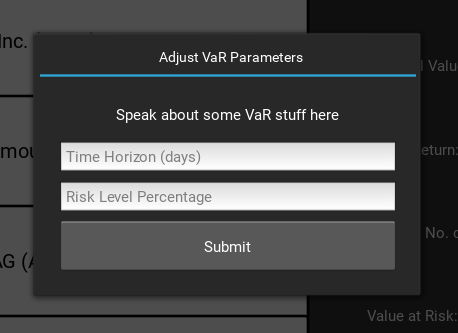
\includegraphics[width=0.7\textwidth]{Images/Term 2 Images/image (11).png}
  \caption{Original Adjust VaR Pop-Up}
  \label{fig:OG Adjust VaR}
\end{figure}

\begin{verbatim}
  class AdjustVaRPopup(Popup): 
      def __init__(self, portfolio, varCalc, **kwargs):
          super().__init__(**kwargs)
          self.varCalc = varCalc
          self.currentPortfolio = portfolio

      def submit(self):       
          self.varCalc.timeHori = int(self.timeHoriInput.text)
          self.varCalc.rlPercent = float(self.riskLevelInput.text) / 100.0
          self.currentPortfolio.initialStockTotals()
          self.dismiss()
\end{verbatim}

\vspace{0.3cm}
With this pop-up, it passed in the current instance of the portfolio class and the varCalc class being used inside it. With his, it could directly change the VaR calculator class by adjusting its parameters directly, as well as updating the new VaR totals to reflect these new changes, applicable for both Monte Carlo Simulation and Model (Variance-Covariance) methods. I knew that not everyone that uses this app could understand what Value at Risk even represents or means in general, so I decided to add a brief explanation of what it is in the form of a contextual sentence as can be seen in figure \ref{fig:Final Adjust VaR}. I used colour coordination to make it easier to understand what text input relates to what portion of the sentence, making use of hint text colour, and for both pop-ups featuring inputted data (the other being \texttt{InputStock}), I added full verification and visual animations to help emphasise when either text input was incorrect. The numbers within this sentence will also update every time the pop-up is re-opened, so the user will always know what values are currently selected. I know that it would be better to show this on the Portfolio screen at all times, but I was not able to find a subsequent place that I could showcase such information, so it's current location will have to suffice.\\\vspace{0.3cm}

\begin{figure}[h]
  \centering
  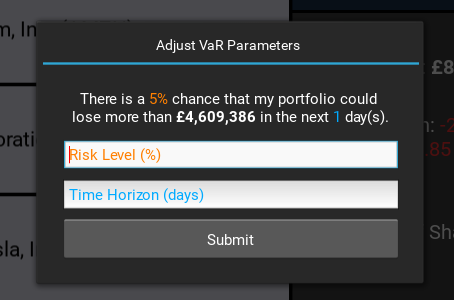
\includegraphics[width=0.7\textwidth]{Images/Term 2 Images/Final Adjust VaR.png}
  \caption{Completed Version of Adjust VaR Pop-Up}
  \label{fig:Final Adjust VaR}
\end{figure}

\subsection{The Finalised Portfolio Screen}
I am inherently not the best at creating visually appealing software, I struggle with finding colour schemes that are coherent and I don't know how to always make things look right. With my VaRChecker, I was able to find a bland gray scheme, and whilst I continued to utilise a few of these colours for consistency, I settled on a range of different blues for the portfolio screens display. I have made a multitude of different styling and customisations to help with visual appearance and user understanding of where things are and what is important. The portfolio's code has been adapted to work when there are no stocks being held within it, and when there's only one stock being held as well, since yfinance downloads need to be defined differently afterwards when retrieving information since it gives it back in a different data-frame. For a while, I was dividing my VaR Method Simulation by 100 since I used the same code from my \texttt{VaRChecker.py} file, but after realising and changing this, I was able to get matching VaR results across the two screens, so both produce accurate single stock data. The screen is fantastically robust and can handle whatever stock storage scenario you want to throw at it, including storing large stock names and numbers. I will add a range of figures showing various parts of this screen below, this also including \ref{fig:Final Adjust VaR} since that is from the finished product as well and a previous green button design that I didn't think fit the visual style, as well as me not having changed the Stocks to a Blue Hue.\\\vspace{0.3cm}

\begin{figure}[h]
  \centering
  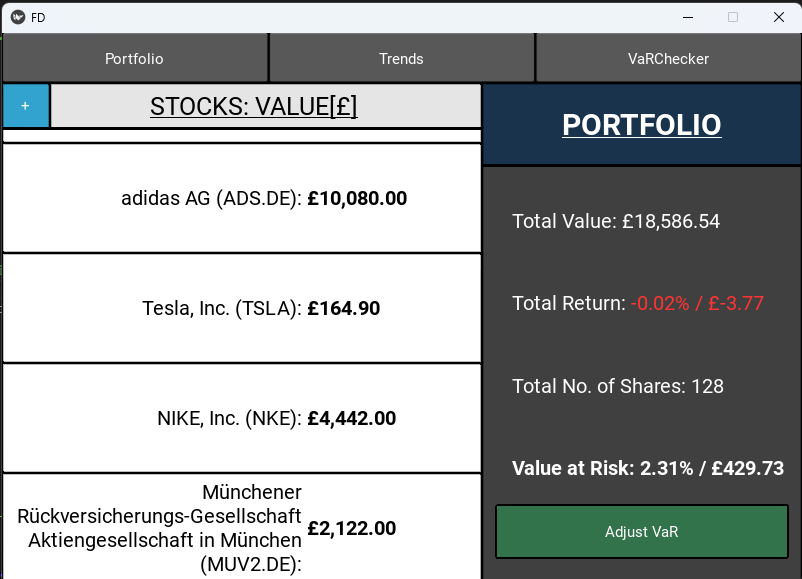
\includegraphics[width=0.7\textwidth]{Images/Term 2 Images/image (8).png}
  \caption{Previous Iteration of Portfolio Screen}
  \label{fig:Previous Iteration}
\end{figure}

\begin{figure}[h]
  \centering
  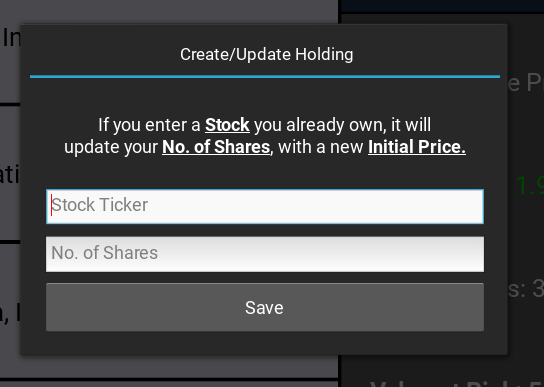
\includegraphics[width=0.7\textwidth]{Images/Term 2 Images/Create Holding.png}
  \caption{Final Create/Update Holding Pop-Up}
  \label{fig:Final Create Holding}
\end{figure}

\begin{figure}[h]
  \centering
  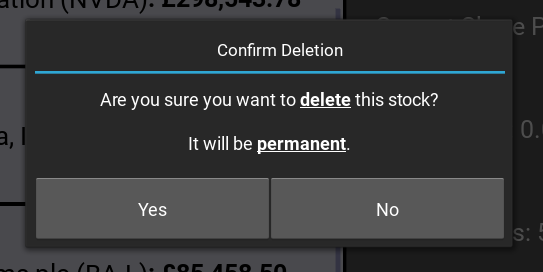
\includegraphics[width=0.7\textwidth]{Images/Term 2 Images/Confirm Delete.png}
  \caption{Final Confirm Delete Pop-Up}
  \label{fig:Final Confirm Delete}
\end{figure}


\begin{figure}[h]
  \centering
  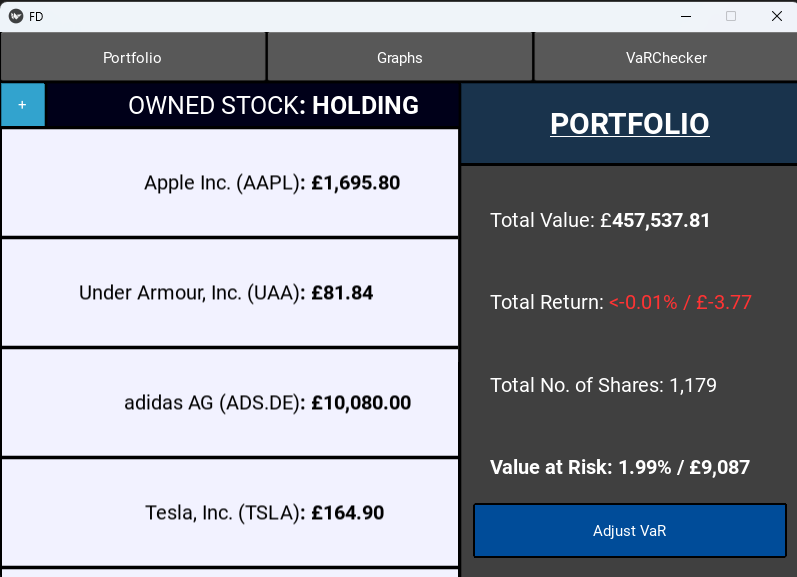
\includegraphics[width=0.7\textwidth]{Images/Term 2 Images/image (6).png}
  \caption{Completed Portfolio Screen}
  \label{Completed Portfolio Screen}
\end{figure}

\section{Chapter 5 --- Graphical Visualisation}

\subsection{Convergence Analysis}
After finishing my Portfolio screen, I realised that the term "Trends" for my final screen was not sufficient for what I wanted it to be. Thus, it was changed to "Graphs", particularly influenced by a brief detour I took within my recent development cycle, when I created a graphical representation of my Monte Carlo Simulation.


\subsection{Matplotlib within Kivy}

\subsection{Creating the Graphs Screen}
Start with putting my initial drawing for this here.

\subsubsection{lots of these}

\subsubsection{lots of these}

\subsubsection{lots of these}

\subsubsection{lots of these}

\subsection{The Finalised Graphs Screen}


\section{Chapter 6 --- Completed Deliverable}

\subsection{Features and Expected Use}


\subsection{Final GUI Design}

\subsection{P-Values and Graphical Analysis}


\subsection{Adaptations for Packaged Release}






\section{Chapter 7 --- Software Engineering}

\subsection{Object Oriented Programming}

\subsection{Design Patterns}

In developing my Initial Design for my Graphical User Interface (GUI) to calculate VaR, I have employed several design patterns that facilitate a robust, scalable, and maintainable codebase. Below are key design patterns utilized within my application:\\\vspace{0.3cm}

\underline{\textbf{Model-View-Controller (MVC)}}\\\vspace{0.3cm}

For my final iteration of my Initial GUI Design, the architecture loosely follows the MVC pattern, segregating the application logic (Model), user interface (View), and input control (Controller) into separate components. This separation enhances the application's ability to handle user interactions and data manipulation independently.

\begin{itemize}
    \item The \textbf{Model} is represented by the data retrieval and VaR calculation logic, which fetches financial data and computes the VaR and back-testing estimation.
    \item The \textbf{View} is the user interface, designed with Kivy's layout and widget system, providing a responsive and interactive experience.
    \item The \textbf{Controller} is evident in the event-handling methods, like \texttt{populateList} and \texttt{generateVaR}, which respond to user inputs and trigger model updates.
\end{itemize}

\underline{\textbf{Observer Pattern}}\\\vspace{0.3cm}

The Observer pattern is present in the way the application monitors the state of user inputs. For instance, toggle buttons for selecting the VaR calculation method employ event listeners that update the system's state when user interaction occurs.

\begin{verbatim}
hButton.bind(on_press=self.simMethodPressed)
mButton.bind(on_press=self.simMethodPressed)
\end{verbatim}

This pattern decouples the system's components, allowing for independent updates and scalability.\\\vspace{0.3cm}

\underline{\textbf{Command Pattern}}\\\vspace{0.3cm}

The Command pattern is utilized in encapsulating the action to be performed in response to user interactions. For example, when a user selects a stock or initiates a VaR calculation, the corresponding actions are enclosed within command methods, such as \texttt{populateList} or \texttt{generateVaR}.

\begin{verbatim}
button.bind(on_release=lambda btn, i=i: ...)
\end{verbatim}

This approach allows for more flexible and extensible execution of actions within the application.\\\vspace{0.3cm}

\underline{\textbf{Singleton Pattern}}\\\vspace{0.3cm}

While not explicitly implemented, the Singleton pattern is conceptually used in the management of the application state. There is only one instance of the \texttt{ApplicationView} class, which maintains a single state throughout the application's lifecycle.

\begin{verbatim}
class IDTApp(App):
    def build(self):
        return ApplicationView()
\end{verbatim}

This ensures that there is a consistent state that is accessible throughout all parts of the application.\\\vspace{0.3cm}

These design patterns contribute significantly to the application's robustness, allowing for efficient risk assessment and providing a foundation for future enhancements and scalability.By adhering to these established practices, I have ensured that my software remains maintainable and adaptable to the evolving needs that my graphical interface my undergo in the future.



\subsection{Testing and Documentation}

Testing is a critical component of software development, essential for ensuring that the application meets its requirements and is free of errors. Mainly for my project, the primary mode of testing involved running the application and observing its behavior for errors or incorrect VaR calculations.\\\vspace{0.3cm}

This testing approach used can be classified as Ad Hoc Testing and Exploratory Testing. These methods are informal and unstructured, as I have been relying on my intuition and experience to identify issues.

\begin{itemize}
    \item \textbf{Ad Hoc Testing}: This type of testing is carried out without any formal test plan or test case documentation. It is a random examination of the application, often useful for discovering glaring issues quickly.
    \item \textbf{Exploratory Testing}: This approach combines learning, test design, and test execution into a single activity. It is particularly effective in situations where there are no detailed specifications, and tests need to be devised on the fly.
\end{itemize}

While these methods can be effective for identifying obvious faults, they lack reliability and cannot provide a systematic approach that other testing methods would. They are often more suited to the early stages of development which this project is still in, thus me using them so far.\\\vspace{0.3cm}


One of the main limitations of my current testing approach is the absence of \textbf{Test-Driven Development (TDD)}. TDD is a modern software development process where requirements are turned into very specific test cases, then the software is improved to pass the new tests. This approach was not followed, as I was unable to justify what I would be testing for (I had planned out unit testing, but I especially did not know how to incorporate it within a Kivy application, as I have not done TDD with Python or Kivy before), so I continued with the above testing style, which worked and allowed me to create my program efficiently, but not up to the industry standard that I know I should be aiming for.\\\vspace{0.3cm}

\newpage
For future development cycles, I plan on incorporating more testing strategies to enhance the quality and reliability of the application, such as:

\begin{itemize}
    \item \textbf{Unit Testing}: Develop tests for individual components or functions to ensure they work correctly in isolation. (Had already planned, now I shall be able to implement)
    \item \textbf{Integration Testing}: Test the interactions between different parts of the application to verify that they work together as intended (Happened during my Ad Hoc Testing often, but need to be able to explicitly show that that's what I was testing for).
    \item \textbf{Automated Regression Testing}: Implement an automated test suite that can be run regularly to catch regressions early in my next GUI's development cycle.
    \item \textbf{Performance Testing}: Evaluate the application's performance, especially when handling large datasets or performing complex calculations, to ensure that it meets the necessary speed and efficiency requirements, especially when I incorporate multiple stocks, portfolios, and full searching capabilities into future applications.
    \item \textbf{User Acceptance Testing (UAT)}: Involve end-users to validate the functionality and usability of the application in real-world scenarios (Will bring in external individuals to help be observed, providing a wide range of feedback that I can take note of and apply to my application).
\end{itemize}

By integrating these practices, my project can achieve a higher level of quality assurance and deliver a more robust and user-trusted VaR product.

\subsection{Version Control (Git)} 

Version control is a system that records changes to a file or set of files over time so that specific versions can be recalled later. In this project, I have had Git employed as the version control system for everything I have done.
Git is a distributed version control system, which means that the complete codebase and history are available on every developer's computer, allowing for easy branching and merging. My approach to using Git was straightforward:

\begin{itemize}
    \item Regular Commits: Consistent commits were made to the repository, with detailed messages that clearly described the changes and their impact on the project.
    \item Backup and Security: All the code was backed up on OneDrive as well (a personal decision), providing an additional layer of security and ensuring that no work would be lost in case of system failures.
    \item Branching Strategy: While currently the project has not utilised extensive branching, I acknowledging the  benefits of feature branches and plan to rigorously employ them in the future.
\end{itemize}

The practice of making regular commits with detailed messages is incredibly invaluable, thus me making sure to regularly comply with this methodology. It enabled the tracking of changes and helps simplify the process of understanding the evolution of the codebase. For me, Git has been essential for several reasons:

\begin{itemize}
    \item \textbf{Reversion}: Git can allow me to revert to previous states of the codebase, which is crucial when a new feature can accidentally break functionality.
    \item \textbf{Traceability}: With Git, all my changes are traceable to a specific commit, making it easier to track when and why changes were made.
    \item \textbf{Backup and Restore}: My files are backed up on a remote repository, providing a fail-safe in case the my local repository suffers a setback.
\end{itemize}

While my development with this project's version control strategy was effective to a degree, it also highlighted areas for improvement. Adopting a more structured approach to branching and leveraging the full suite of features offered by Git will be a focus in future endeavours to ensure a more efficient and error-preventative development workflow.

\subsubsection{Branching and Tagging}

\section{Chapter 8 --- Critical Analysis}

\subsection{Interim Evaluation}
In the end, for this term, I am still happy with the progress I made. I learnt some very valuable lessons, such as needing to make sure that I do all of the documentation alongside the coding, since with the gap in progress, it can become tedious to try and explain it all properly in the future. I feel that I accomplished the goals set out within my original timeline for what I wanted to achieve this term, for this interim report, and whilst there are sections of this report that I am unhappy with the result of (especially the final iteration of the GUI), I am still satisfied with the report as a whole in displaying what I had learnt and the code I was able to create, especially with the inconsistency with my physical and mental health experienced over the last few months. I also am aware of my lack of testing that I have performed, I spent a large chunk of time just testing everything myself to make sure it works, when I should have been following a better framework, I plan to learn from this and change the way I develop and document the code come next term. I know the Latex is not great in this document, its still the first time I've ever done large scale documentation like this before, but hopefully by the time my final report is complete I will have given myself enough time for it to be at an acceptable level. I also know I haven't used enough sources, the sources that I did use were so useful that I kept referring back to them, which makes my ability to reference them rather bland, so I will also make sure to diversify with many more references in the future. With how the final design for the initial GUI came out, I'm extremely happy with its functionality, its very fast and easy to use and produces the exact results you need whilst still being robust. There's still a lot to work on for it in the future, like adding different windows/views, incorporating multiple stocks VaR calculations (I wrote a program to do multiple stocks but I didn't have the time to include that in this documentation either, can be found within my Git project/submitted programs) and allowing you to access entire portfolio's within the application. What I made this term was a great proof of concept for what I can do with Kivy, for my final report I want to be able to do so much more, since that is my main goal, the development of an industry grade application for Value at Risk as well as financial management in general. Finally, there were many planned sections of this report that were never completed, I aim to be able to structure my documentation so that I can complete everything I need in the following term, so to conclude, I am extremely happy with everything I was able to do, but I plan on doing everything much better in the future, as I know it was not optimal enough for what I want to achieve...


\subsection{Final Report Evaluation}

\subsubsection{Coding Achivements and Success}

\subsubsection{Difficulties and Improvements}


\subsection{Conclusion}


\section{Professional Issues}

\subsection{Plagiarism and Using AI}

\subsection{Finance Industry Ethics}




% \subsection{VaR and what it is in the industry atm, and other VaR softwares and how I can take inspo from them?}
\newpage
\section{Bibliography}
\subsection{References}
\begin{small}
\begin{enumerate}
  \item\label{ref1} Alexander, C. (2008). *Market Risk Analysis: Value-at-Risk Models.* Hoboken, NJ: Wiley. [Online] Available at: \url{https://ebookcentral-proquest-com.ezproxy01.rhul.ac.uk/lib/rhul/reader.action?docID=416450}.
  \\\textit{This book covers various aspects that I want to approach in this project, such as historical simulation, Monte Carlo simulation and various forms of testing that could be highly useful for my project.}
  
  \item\label{ref2} Arbuckle, D. (2017). *Daniel Arbuckle’s Mastering Python: Build Powerful Python Applications.* Birmingham, England: Packt. [Online] Available at: \url{https://learning.oreilly.com/library/view/daniel-arbuckles-mastering/9781787283695/?ar=}.
  \\\textit{I chose this reference as it helps with python packaging, being able to turn a python code and all its GUI and libraries into a single executable file, which is something I want to be able to do for this project.}

  \item\label{ref3} Choudhry, M. (2006). *An Introduction to Value-at-Risk.* Chichester: John Wiley \& Sons Limited. [Online] Available at: \\ \url{https://learning.oreilly.com/library/view/an-introduction-to/9780470017579/}.
  \\\textit{Covers similar topics to the first reference, but seems to go into more detail on specific issues that I may need to address in this project.}
  
  \item\label{ref4} Duffie, D. and Pan, J. (2019). *An Overview of Value at Risk.* [Online] Available at: \url{http://web.mit.edu/people/junpan/ddjp.pdf}.
  \\\textit{A much shorter reference, it is a paper that covers the basics of Value at Risk, which I will be using to help me understand the fundamentals of the topic since I have been able to follow it better then the other references.}
  
  \item\label{ref5} Föllmer, H. and Schied, A. (2016). *Stochastic Finance: An Introduction in Discrete Time.* Berlin: de Gruyter. [PDF]
  \\\textit{A recommended reference from my supervisor, it is a book that covers higher level concepts relating to my project but also provides an overview of stochastic finance in general, which I have seen to be useful in understanding the topic.}
  
  \item\label{ref6} Hull, J.C. (2008). *Options, Futures, and Other Derivatives.* Upper Saddle River, NJ: Prentice Hall. [PDF]
  \\\textit{This is my main reference for the project, as it is the main textbook suggested. It has a relevant chapter on Value at Risk, which explores many of the different aspects that I will need to look into for this project.}

  \item\label{ref7} Pritsker, M. (1997). "Evaluating Value at Risk Methodologies: Accuracy versus Computational Time." *Journal of Financial Services Research* 12: 201-242. [Online] Available at: \url{https://doi.org/10.1023/A:1007978820465}.
  \\\textit{Another short reference, this is a paper that compares the accuracy and computational time of various Value at Risk methodologies, which I will be using to help me understand the different methodologies and how I can apply them to my project in the most efficient manner.}

  \item\label{ref8} Raman, K. (2015). *Mastering Python Data Visualization: Generate Effective Results in a Variety of Visually Appealing Charts Using the Plotting Packages in Python.* Birmingham: Packt Publishing Limited. [Online] Available at: \url{https://learning.oreilly.com/library/view/mastering-python-data/9781783988327/?ar=}.
  \\\textit{This reference covers various aspects of data visualisation, which I will be using to help me understand how to best display important information in a visually appealing way for my project.}

  \item\label{ref9} Ulloa, R. (2015). *Kivy - Interactive Applications and Games in Python - Second Edition.* Packt Publishing. [Online] Available at: \url{https://learning.oreilly.com/library/view/kivy-interactive/9781785286926/?ar=}.
  \\\textit{This reference is not being used for its content on game development, rather Kivy is a framework that can help create a GUI that works on both desktop operating systems as well as mobile operating systems, which I think I would like to explore the possibility of when developing the application.}

  \item\label{ref10} Weiming, J.M. (2015). *Mastering Python for Finance: Understand, Design, and Implement State-of-the-Art Mathematical and Statistical Applications Used in Finance with Python.* Birmingham, England: Packt Publishing. [Online] Available at: \url{https://learning.oreilly.com/library/view/mastering-python-for/9781784394516/}.
  \\\textit{This reference covers various ways of handling financial data within python, which I will ensure to help me understand how to best handle the data I will be using within my project.}

  \item\label{ref11} Wasserstein, R.L., \& Lazar, N.A. (2016). *The ASA Statement on p-Values: Context, Process, and Purpose.* The American Statistician, 70(2), 129-133. [Online] Available at: \url{https://www.tandfonline.com/doi/full/10.1080/00031305.2016.1154108}.
  \\\textit{This reference is crucial for understanding the nuanced interpretation and use of p-values in statistical hypothesis testing, since it is  relevant for the back-testing aspect of my project involving the VaR model validation.}

  \item\label{ref12} Casarin, R., Chang, C.-L., Jimenez-Martin, J.-A., McAleer, M., Pérez-Amaral, T. (2013). *Risk management of risk under the Basel Accord: A Bayesian approach to forecasting Value-at-Risk of VIX futures.* Mathematics and Computers in Simulation, 94, 183-204. ISSN 0378-4754. [Online] Available at: \url{https://doi.org/10.1016/j.matcom.2012.06.013}.
  \\\textit{This reference is useful for understanding the Bayesian approach to forecasting Value-at-Risk of VIX futures and its relevance to risk management in financial institutions.}

  \item\label{ref13} Kivy. (2023). *Kivy Documentation.* [Online] Available at: \url{https://kivy.org/doc/stable/}.

\end{enumerate}
\end{small}

\subsection{Literature Review}

The bibliography that I have provided helps me to summarise some of the key literature surrounding Value at Risk (VaR), encompassing foundational theories, methodological advancements, and practical aspects of VaR in financial risk management, as well as touching on python and its plethora of libraries. It integrates perspectives from seminal texts, empirical studies, and modern computational approaches.\\\vspace{0.3cm}

Foundational knowledge on VaR can be derived from Hull (2008) [\ref{ref6}] and Choudhry (2006) [\ref{ref3}], focusing on its mathematical underpinnings and historical context. Alexander (2008) [\ref{ref1}] provides detailed insights into various VaR methodologies, complemented by Pritsker's (1997) [\ref{ref7}] empirical analysis on their competence.\\\vspace{0.3cm}

The practical implementation of VaR models using Python is guided by Arbuckle (2017) [\ref{ref2}] and Weiming (2015) [\ref{ref10}], highlighting Python's utility in financial data handling and visual representation. Ulloa (2015) [\ref{ref9}]  adds a modern perspective with multi-platform graphical user interface applications that are applicable to help display and increase the accessibility for financial risk assessments associated with VaR.\\\vspace{0.3cm}

Recent discussions around VaR and statistical analysis are enriched by Wasserstein and Lazar's (2016) [\ref{ref11}] exploration of p-values in statistical hypothesis testing, relevant for VaR model back-testing. Casarin et al. (2013) [\ref{ref12}] introduce a Bayesian approach to VaR, showcasing the evolving methodologies in response to financial market dynamics.\\\vspace{0.3cm}

Overall, I think the references I have chosen really help encapsulate the multifaceted aspects of VaR found in the modern age, highlighting its theoretical, methodological, and practical scale. It highlights the continuous evolution in VaR modelling, helping set the context for my further research into this field, as well as helping enhance my knowledge for user interface design and general industry standard financial risk software development.

TALK ABOUT THIS STUFF MORE, ADD MORE ABOUT IDK NEW REFERENCES AND GO INTO MORE DETAIL, LIKE CALLUM

% TEMPORARY END OF DOCUMENT TO PROVIDE MORE REALISTIC WORD COUNT FOR NOW
\end{document} 

\section{Appendix}

\subsection{Example Graphs}

\subsection{Diary}
FINAL YEAR PROJECT DIARY\\
 ------------------------------------------------

28/9/23 - Start of Project\\
Today, I am starting this project. I have finally fully recovered from a health issue I was having at the start of term, but I am still dealing with an ongoing emotional issues that I will have to push through to complete this project successfully (heartbreak).\\\vspace{0.3cm}

01/10/23 - Setting Up LaTeX\\
I have been able to get Latex working for my Documentation, after having various problems with the version of LaTeX I installed not working with VSCode. I finally used Latex Live and was able to get it working, thus have created a test document to ensure it works. I have started researching and acquiring sources for my project, and will need to ensure I complete the Project Plan accordingly.\\\vspace{0.3cm}

17/10/23 - Fixing my DIARY\\
Due to illnesses (that are still ongoing), I have not been able to properly update this diary to a satisfactory level. When my illness has rescinded, I will be able to start continuously updating this diary with my projects progress...\\\vspace{0.3cm}

11/11/23 - Finally being able to get on with working\\
Have finally gotten illnesses and emotional issues under control, and have been able to start working on my project. I've used the sources I originally found to help me understand VaR for historical simulation and variance covariance model methods, whilst also using trial and error to create two test programs to test the methods. I need to start on the documentation for the project tomorrow with creating the latex for it and making sure to document my progress in understanding var as well.\\\vspace{0.3cm}

12/11/23 - Setting Up Documentation\\
I copied over my documentation for the Project Plan, and used it as a baseline for me to establish what I need to be in my interim report. Taking brief reference from an email that Argyrios sent, and combining it with what I already had from my previous plan (timeline), as well as making sure I include everything needed from the mark scheme, I created the contents and headings for my documentation going forward, so I know what I need to add into each section up until the completion of the interim report. I now need to start populating the information before I continue to progress with the project too much, however for this week in my original plan I was supposed to research and understand back testing, however I think I will wait slightly so that I can catch up on documentation, since I really should have been documenting my testing on getting the VaR methods to work in the first place, so I will make sure to complete the prior sections (I think I'll skip on the introduction documentation at the moment too so I can focus more on getting the documentation done for the code, so that I can then progress with more coding).\\\vspace{0.3cm}

13/11/23 - Back-testing\\
I said that I would do more documentation next, but I wanted to briefly read on back testing. Upon doing so, I saw that it didn't look to challenging, so I thought I'd quickly try and implement it for historical simulation. I was able to do so, which means I should be able to adapt it for the model method tomorrow quite easily, I also found that the back testing seemed to think my VaR calculated was accurate at the 5\% level, but when changing it to 1\% level it was not as accurate, so I will need to look into this further tomorrow as well, see if its to do with assuming that my returns are normally distributed, or if its something else.\\\vspace{0.3cm}

14/11/23 - Combined Program for Both Methods, for Single Stock\\
At the start of the day, I implemented the back testing for the model building method, tested it to see if it worked, and saw that it would mainly still fail the back testing. I don't really know what I'm supposed to do with the back testing at the moment, but I will research more into it in the future. I then decided to make a program that I could input all the relevant details into to get VaR results, only accounting for a portfolio of just one stock type, I wanted to have it so the user could choose their one stock from a choice of multiple stocks, so I displayed the FTSE100, let the user choose that and input their portfolio amount, as well as other values, and at the end they would chose what VaR method they would want to use to calculate the VaR. The program displays the VaR and back tests it afterwards, but almost 90\% of the time it would fail the back test. I assume this is due to these methods not being the most robust for calculating VaR, or for I'm performing the back testing wrong, but regardless everything else in the program seems to work, and this program can help me in the future when I implement a GUI, my initial one will most likely only handle one stock type, so I can use this program as a base for that.\\\vspace{0.3cm}

24/11/23 - GUI + Finalising some statistical analysis + Documentation\\
Have not been able to update the last week or so due to illness again, have gotten around to continuing to work on the project. I have been using a reference book to research on how to use Kivy for the GUI, I am giving myself a few days to understand and implement that. I have been in contact with my supervisor, and they have helped me in better understanding the statistical analysis that I need to do when back testing, I still don't 100\% have a grasp of it, but I know that I will need to be able to utilise it better in the future. Finally, I think I've finalised what I need to be in the documentation, and I really need to start on it soon, so I will do do that soon too hopefully.\\\vspace{0.3cm}

29/11/23 - Initial GUI close to completion\\
I had been struggling to get started on the GUI, as in I have been working through the book/recourse I had on it but I still didn't know where to start. So I experimented with what I had learnt and managed to create an initial design based on a sketch I made for the application. With this initial design, which was not populated with any functionality, I have been gradually adding bit by bit of what I need to be able to generate my single stock VaR results. I know it's not multi-stock but after being able to create this initial GUI design and learning Kivy, I'll be much more confident in creating further kivy applications in the future. The final thing I need to do for it now is to have it actually generate the VaR results, display that it has done back testing and some indication of the significance of the result, as well as text box validation so it is easier for the user to use. Then I will have to quickly create my presentation, which will involve slides explaining VaR, what my aims are for the project as well as a showcase of what my final GUI can do, I think, I will need to go over the specification for it in more detail tomorrow. Still a lot to do and I'll have to work as hard as I can over the next week to ensure I complete it all appropriately.\\\vspace{0.3cm}

30/11/23 - Implemented VaR and Back Testing and fixed a lot of problems\\
I was having issues when I used my laptop to create the application, since it broke all the formatting. Upon testing around, I discovered that depending on the monitor size (since they have the same resolution the two displays I use), it will change the size of the kivy application. I didn't want this, so I found out using DPI aware will mitigate this issue and allow to be more accessible everywhere. I implemented my VaR code from the command line program, and it works well. I also discovered that many of the stocks don't work from the FTSE or maybe the trackers are out of date. Regardless, I'm thinking of maybe displaying a different list of stocks, but I will decide on that tomorrow. I have implemented back-testing, but I don't think its all working properly and I need to use tomorrow morning to get it to be represented in some fashion on the application. After that I think I am happy with the initial GUI design and I will begin work on the presentation, since with the GUI complete, I can make sure to be able to show it off.\\\vspace{0.3cm}

02/12/23 - Completed GUI and Created presentation\\
After performing more test on the back-testing, I found that me thinking that it wasn't working properly was an outlier that gave a very large p-value, in general the back testing appeared to be very accurate and helped a lot with the statistical analysis and being able to disprove/approve the hypothesis's proposed with each VaR. I also added better verification to the text inputs, so that when you write any numbers or letters that don't make sense, it will just default the values. I also had previously commented on not being able to access many of the other stocks with yahoo finance, but I had seen evidence of all the FTSE100 being listed on the yahoo finance website, so after doing even more research I discovered that a lot of the stocks have a .L listed with their ticker, so I got it so that every time it would fail to download a stock, it would attempt to re-download the stock with the additional '.L', and this managed to work for every single FTSE Stock, so now the program feels more complete now that every stock is accessible. I managed to add a few more bits of verification, to help with some of the stocks returning bizarre results, so they can be accounted for in the future if it happens as well, and to make sure my program never crashes. Finally, I was able to create my presentation, I am happy with how it looks even though I did have to rush certain sections but it still looks great and I should be able to describe everything well. All I have to do now is most of my documentation, I had been severely behind on it, so I'll see if I can catch up. Also comment on forgetting to use a different branch for the GUI.\\\vspace{0.3cm}

06/12/23 - Documentation\\
I have spent the last few days working hard on the documentation. I regret not being able to do this as I progressed with the project, since now it will be hard for me to show the development of certain aspects properly. Regardless, I do not have much more time before this is due, so I wouldn't have been able to say/show everything I wanted for each section anyway. I am sad that I have so much that I need to show off/write about within my report(s), but I feel that due to the circumstances with my health and emotional issues this term, I was unable to create work that I feel is satisfactory to the standard I hold myself to. I've been able to mostly complete the first section of my documentation, I think, and I've gotten onto where I am finally talking about code. I want to include a lot of screenshots to show things visually, but using latex is a lot slower then word, with you having to save your pictures in a certain directory, and then having to reference then within latex, with word just letting you copy and paste in comparison. Maybe I would've been able to do more consistent documentation alongside my coding if I was able to do it within word, I will keep that in mind for next term, maybe use word whilst I go along with the development, and then transfer it over to latex at the end. I will continue to work on the documentation tomorrow, and hopefully I will be able to complete it all by the end of the day, so I can submit it and then perform my presentation the following day.\\\vspace{0.3cm}

07/12/23 - Finale\\
I have finally completed the documentation, I am unhappy with the fact I had to miss out on so many sections that I had planned, but in the end I'm rather blown away that I was able to consolidate and present so much in such a small amount of time. I'm proud of the result, of this report and the code I created this term, but I do plan to spend the majority of my holiday catching up on the time I feel that I lost for my project throughout the term due to my illnesses and heartbreak. I need to compile all the programs I think are relevant for my submission, and put them all together within a zip file to be submitted. I am also dreading my presentation, as I know I will be quite sleep deprived for it, but I am happy with the slides I made, and I hope to be able to justify my project well, especially after I was able to justify it so well within the interim report/documentation. There are many changes that I want to make, but for now I will finally take a bit of a break to recover from the excessive amount of work that I have put in before the deadline to achieve this. Thank you for reading for now...

29/01/24 - Start of Term 2\\
I have discovered testing over the winter break that it displays properly on my normal monitor, but not on my laptop, even though I have fixed the resizing issues. I need to make sure to take screenshot references for this, and write about it within my FYP documentation.\\\vspace{0.3cm}

05/02/24 - Fixing the issue from the last term\\
I worked out what the issue was with my program. Essentially, I had hard coded the structure of a lot of the layouts, by not using size\_hints for everything, since that would keep everything consistent no matter what window size. Because of this, I need to change everything to implement size\_hints, which helped fix overall layout, but there would still be problems with text and other objects that I had hard-coded on the Python side that I couldn't use hints for, such as font size. This is where sp (scale independent pixels) came in handy, since I could use this to change any of my hard-coded values into ones that scale (which I could've done to fix the previous problem but it was better for me to get used to using hinting with the change). After attributing the dp to all integer size values, I had essentially gotten the program to work on both of my monitors, so I decided to stop using the DPIaware command, just let my program adjust naturally. I think I want to have the window be resizable in the future, but for now I want to get the tabbing system working next. I also need to quickly fix the back-testing title label I have for it, since I know where I want it to be, its just hard to add it to the layout properly...\\\vspace{0.3cm}


19/03/24 - Finished Researching Monte-Carlo simulation\\
After a busy month, with lots of other coursework and external factors, I have now finally been able to return to focusing on my project for the final stretch needed. I have now researched and understood the Monte-Carlo simulation, so I will start by creating a simple Monte-Carlo command line program to test that my knowledge lines up with creating it within Python. After that, I will start implementing tabs for the program, so I can move on to adding more utilities for the program, as well as implementing Monte-Carlo within it too.\\\vspace{0.3cm}

23/03/24 - Implemented MonteCarlo\\
I created a separate command line application to test that I could properly get MonteCarlo Sim to work, which I was able to. I'm planning to implement it into the main program after I've done the tabbing system.\\\vspace{0.3cm}

25/03/24 - Implemented Tabbing System and OOP + Folders\\
I managed to find a source that explained how screens work within Kivy, helping me set up a screen manager, and attempt to swap between multiple screens. At first, this absolutely broke my deliverable from last term when I ported it into a screen, but I realised that it didn't have the original box layout support that I had defined it with on the python side. So I had to implement that within the kv file and it seemed to work with the same functionality. I set up generic buttons for tabs at the top, but I don't like how they looks, so I will try and change them if I have time in the future. I like the custom animation that Kivy seems to have when switching between screens, but I don't like that it only moves in one direction, so I may also try and adjust it so that it will slide a certain direction depending on which screen you're navigating from to. \\Finally, I decided that I wanted to make the project and coding more Object Oriented, to allow it to be easier to understand and maintain the codebase in the future. To do this, I realised I can easily import the python code into a main python file, which allowed me to separate all the screens I now wanted all into their own individual files, including last terms deliverable, which I have now called a VaRChecker (which I still need to implement Monte-Carlo Sim into). I also, after performing some tests to make sure it worked properly, have been able to separate up the kivy (kv) files so they all communicate but are still separate files, so everything is split, communicates, and runs properly. I assume that when I compile this all into a working application in the end it will all be fine but I will have to see then. For now, I am going to start working on the Portfolio page as fast as I can, since I feel like it is one of the most important, complex features and I need it to work robustly. \\\vspace{0.3cm}

28/03/24 - Started creating Portfolio Screen\\
Today I started working on the portfolio screen, I wanted to make sure the functionality and aesthetics of this part were satisfactory but I am bad at making the aesthetic work properly, so for now I'm just focusing on functionality. I used some conceptual sketches that I will probably add to my report, and I've made a rough version of what I want to screen to look like, based off of it. Its very early stage, so it doesn't look very good but I'm hoping to add to the functionality, so it can work sufficiently.\\\vspace{0.3cm}

03/04/24 - More Portfolio Screen + Removing Rankings Screen + Caching storage\\
I found out you can use JSON.store to create a way to essentially cache portfolio information that I want to be retained within the program. This is amazing, as now I can store bits of information and keep it there, so the program can have initial stocks prices, and compare back to them whenever. I also realised that I just do not have the time to be able to create the 3 extra screens that I was planning to make for this term, so I'm just going to have to create 2, to be honest, the third screen I was going to make I didn't have a very good plan/idea for either, so doing it this way has streamlined the options that I have available, which is good, I'm feeling more confident that I can complete my goals. \\The two screens I'm keeping are trends and portfolio (the main one), and I am not going to be doing rankings any more. I was having a problem with labels not displaying when being put on my stock buttons, but I fixed this by directly adding text to the button, although it doesn't look very good regardless so I'll definitely have to change it in the future. I was then able to finally integrate yfinance into the current code, there was a massive error to do with the .info section, when researching online, there were no ways to fix the issues other then pulling custom code from other people's GitHub to fix, but I realised that I can just download the stocks and grab the latest value, and that gave me the results I needed anyway, so bizarre. I wanted to get it so that I would get consistently updating information every minute for fresh stock data, whether I was looking at an individual stock or all stocks. \\TO do this, I used a clock feature that would loop, and set up variable checkers to see if the other one was active or not, if so, it would turn off one clock and start the other, making sure only one can loop at a time and acquire fresh stock information. I've got it so it creates the totals, the returns and everything by comparing current prices to the initial prices, this is great as I can leave the stocks in their storage for now and it will only help show off my program more in the future. I need to get more information shown on the right hand side, like current individual stock price, rather then just the owned amount by timesing by the shares owned. I also have yet to implement any VaR stuff, so I will do that next as well.\\\vspace{0.3cm}

04/04/24 - Adding Monte Carlo + Convergence\\
I first implemented MonteCarlo sim, this was initially a bit annoying since I had to re-download all the stocks so I could recreate the weightings of each of them, but I changed the structure I displayed everything with so that I generate the stocks once at the start, and then get them passed in for every other bit of information. I also first realised that I can't use monte carlo sim for single stock simulations, which was fine since I could just re-incorporate my model method that I used within VaR checker. I got both of these to work so that when the total stocks were being displayed, monte carlo sim was used to calculate it, and model was used for the individual stocks, but I didn't like the amount of fluctuation that my monte carlo sim was displaying when I would get it to run 10000 simulations. It was also incredible laggy, I implemented a timer feature to see it took 4 seconds to generate every time. \\After researching some more, I realised that numpy can generate all the simulations at once with one of its methods, returning it in a structured format, and then I can work out the rest with all the simulations prone, this was so much faster, taking 0.07 seconds for the same amount of simulations, 10000. But I still got the results that were too different for every set of simulations, so I decided to adjust the code again so that it would do multiple bursts of simulations, and depending on how close each burst was to the previous, only when it starts to converge, will I display the result. This convergence point indicates that the simulations are giving similar, and subsequently more accurate results towards a specific outcome, which is what we're looking for. I set the convergence point low (0.5\%) to make sure the result was good, and made it so it can perform up to 100,000 simulations if need be, but actually this resulted in my simulations usually being a lot faster, and only sometimes slower then usual, but from what I could to tell, a lot more accurate. \\Finally, I decided to verify how I thought by using Matplotlib to display results of a simulation that continues to run until 100000, thus giving me a good overview to see how accurate it becomes when converging on a certain point over time, and it was good to see this implemented, as the first graphical change I had shown. This was great, but its not a section that I need here on this screen, so I will leave it for now and probably implement it within the trends screen in the future. It got me thinking that I should do the same for the back-testing within my var-checker screen as well, so I will try and do all of that when I work on the next screen hopefully tomorrow. I made a few UI adjustments, fixed up how exiting the pop-up worked and a bunch of other functionality things like being able to click on an invisible button when you select a specific stock to take you back to the total stock display. Overall, a big day for getting back-end stuff to work, now I just need to get this section to look visually better, add a little more information, and I had forgotten to add a way to delete stocks so I definitely need to implement that. I'm aiming to get started on the next screen tomorrow, so hopefully that is how it turns out.\\\vspace{0.3cm}

05/04/24 - StockNameFinder, Delete Stocks, and Portfolio Screen Functionality Completion\\
I started today by being tired of displaying tickers for everything, its practical because its how I want them to be added into my portfolio, but I wanted to find a way to get the name to display it, it would look way nicer. To do this, without using yfinance.info since its broken, I tried web scrapers, first pandas since it can find info in tables in pages, but I couldn't find any pages that would get me the relevant info. So instead, I used beautiful soup, which would help me, when I had sent a request to a webpage, find certain html elements in the page, which let me make requests to specific yahoo websites and look for the html code containing the title of the stock on every page. \\This could only be done since the ticker for each stock is part of the url, which was perfect since they'd all match as its how I get my stock data within python anyway. With this, I was able to retrieve most of the names for my stocks, but it wouldn't work for certain ones for foreign stock exchange, and I fixed it by adding a user-agent to have my request mimic a browser, which seemed to fix the situation. I could now display the names on the stock buttons, and I also got it so that whenever the stock totals (for specific or initial) are displayed with their looping background app refresh, it would also run the load stocks function, passing in the downloaded stock data, so I could then display the current prices of all the stocks without having to re-download them again every time, having everything work together at the same time. Then I added the delete stock functionality, this wasn't too bad, as it just involved me pushing the button originally, and it would see what specific stock is being stored and delete it. \\But since this is deleting, I wanted to add extra verification, so I moved stuff around, had it so a popup appears, the screen info is passed into the class so it can run the initialStockTotals only when a stock is deleted, and made it run all fluidly. This looked great and I don't think I need to change anything about this in the future, it works well so I'm happy. Finally, since this button would disappear whilst I was on the totals page, since it would only need to delete a specific stock when its selected, there was a gap on the screen when it was hidden. I felt that, since my project is about VaR, even though I have a very good VaR working for the screen, I need to give the user the ability to adjust it to some extent, and I think initiating another popup gives me the most freedom to implement and have this happen, since I understand it more after making 2 already. \\I wanted to have two buttons on top of each other that would boolean change which one is active or not at any given time, but this wouldn't let me click one of them, so instead I made it the same button that would send you to a function whenever you clicked on it, and depending on the text at the time (which changed depending on initial or specific stocks), it would perform a different action, either the previous delete functionality, or the new VaR adjustment functionality. The new adjustment one would take you to a new popup, that would have the calculator class passed into it, the one that's initialised and used within the portfolio screen, and you could directly change the time horizon and risk level being used for the VaR. I need to add a lot more verification, finish up that popup and add a lot more visual improvements and quality of life, but functionality wise the screen is looking fantastic.\\\vspace{0.3cm}

06/04/24 - Finishing Portfolio and Starting Graphs Screen\\
I started today by finally getting around and doing proper verification for my inputs. I started with the save stock input, since it needs to check if you're passing in a valid ticker and a bunch of other stuff. This wasn't too hard, since I had verification set up for a similar kind of thing for my previous screen, but to get the logic working perfectly it took a while and some nesting. I also wanted to give visual feedback on entering something wrong, where I discovered the animations feature for kivy, which essentially transitions from one colour to another, for me at least. This was great, because I could quickly get red to flash up and fade, showing they got it wrong. I was having so much trouble with focus shifting not working, not letting me tab from one input to another, but I was able to get it so that it could do that when I clicked the enter key which is good enough for now. Because I liked the animation feature so much, I wanted to add it as a small background transition for how the portfolio looks when going from portfolio to specific stock totals, which looks smooth and helps the user understand whats happening a bit better. \\I wanted to find a way to explain VaR a bit better, so I used the adjustment pop-up for it to write out and explain it, colour coordinating the values displayed to be the same as the text inputs, making it even easier for the user to see what they need to input. I also added verification for these as well, which was even easier to do, since I found out you can use input\_filtering, so I would only let people enter integers for these inputs. All I really needed to do for my screen then was to just fix formatting, I did a bunch of stuff like stopping the stocks from being buttons, instead they're a grid-layout with two columns, so I could wrap the text to be side by side based on the ":", since I thought this would look the most visually appealing, which it does. I had to give them an on click/on press whatever it is, so they could still function like before. \\I changed a bunch of colours all day, going back and forth between different visual ideas, adding boldness and underlining, making the top right have its own border and section, adjusting how close the right and side information is to each other and the left hand side etc. It was all just a bunch of formatting changes, so I think everything looks a lot better now, but I'm not very good at making stuff look pretty, but it will have to do for now. Very proud of the functionality, I added a massive stock name to the portfolio and the app would still display it correctly, works robust. Finally, I've started on the next and final screen that I want to complete for this project. It was originally trends but since I'm not only going to have trends display don the screen, I thought I would change it to be called graphs now. \\I got the original layout working, after I had to look online to find a way to get the imports for having matplotlib stuff within my kivy applications working, they gave me a pip-install and a different way to import the kivy gardens module, but with it working, it all seems to be good. I have a basic graph, displayed, with a scrollable bar underneath, with stock images being used for each option. I wanted to change up the style of having the up and down scrollable sections in my previous screens, so I like how this is, and honestly if I can get this section looking nice, I think I can breeze through the logic of it tomorrow, and finish up, ready to start on the write-up properly by Monday, I HOPE :))\\\vspace{0.3cm}

07/04/24 - Graphs Screen\\
I made an example second graph and tried to add it to the same graph area, but I didn't remove the previous one, so they all got compiled together and it looked very comical haha, they would squish up. Easily solved by adding a clear widget which I had forgot to. I then knew I wanted to get it so that when you hover over points, it would display what those points are, since I knew I would want to show a list of stocks and, to be able to tell which stock is which, I want to display it when you hover over it. This is ambitious, but I really wanted to add the functionality. Unfortunately, its not built into the kivy side of matplotlib with garden, compared to just the matplotlib side, so I was struggling to get anything to work effectively. After doing some research online, I found a single page that had an answer that said would work, so I implemented it and adapted it based on what they had done, and, with a lot of trial and error, I finally got it functioning properly. This looked great, its not 100\% since if you have a graph that has a lot of value near the top, it can sometimes cut into the title and be impossible to see, but I think I'll fix that later if necessary. I was creating a graph every time I had a function, and knew that this wouldn't be efficient, so I took out the creating a graph logic, and made it its own method, making sure to pass the information needed in when it is called. \\This was great because I knew I would have a lot of big complicated code within most graph sections, that I could just call create graph and have that handle the information properly. I essentially created a factory design pattern I think :D I then tired to implement the Monte Carlo Simulation Analysis Visualisation for Convergence that I had made as a method in my Portfolio file, within the VaR Calculators class, but I didn't want to run it from there, I wanted to have all the graphical logic be within the graphs file, so I moved it over. I still needed information from my portfolio page since I was attempting to just create a method to pass it in, so I found a way to call the portfolio and have the information passed in and working for the code, which I then just displayed the values of, working perfectly, I even created a temporary save of the downloaded stocks, so I could just use that data rather then call for stock data again. However, this code, for it to be able to display the amount of simulations I want to show the convergence visually, is incredible slow, making the program freeze for over 10+ seconds every time its clicked. I was so annoyed by this, so I wanted to at least be able to use the rest of my program whilst I waited. \\To do this, I knew I had to incorporate threading/asynchronous programming\\ logic, so I originally tried asyncio, but could not get it working at all, even after updating all my files to be running on the latest version of kivy (I originally had it on 1.9.0 I think became the originally guide that taught me kivy used that), so I decided to use normal threading instead, and it worked, but I needed to use a sleep method to have my code logic run slow enough to even make the rest of the program barely usable whilst it ran. It would also now take a minute, all highly un-optimal but I couldn't do anything about it if I wanted my simulations to look good. This was also annoying since when the threading was running, I couldn't leave the application without it crashing, so I implemented a check to see if I'm trying to close the application, and if so, stop threading. I knew I would want to call portfolio multiple times in my codes future, so I made it a property, that will handle the logic, since it would need to happen after all the screens were initialised, so I can't have it as like a "self" variable, but I also did an on\_enter thing so maybe I can actually, I may try and change that in the future... I disliked the scroll wheel that my portfolio had, so I made a custom one, I need to add it to my original VaRChecker. \\I also took the stock download and displayed a past theoretical total if I had kept these amount of shares with stock pricing from the last 500 days downloaded. This looked great but would display the numbers at the bottom in a confusing way, and I got stuck forever trying to fix it, since it defaults to displaying the numbers from 0-x, but I implemented a check to flip the axis which finally seemed to work. There were also a bunch of gaps between points on the graph, after printing out I saw there were nan values, so I created some code to check for this and create assumed values that make logical sense to me and look good on the graph. I also wanted to display pounds and other symbols with the hover over, so I added that as something saved and shown as well. On a whim, I decided to research a way to get my monte carlo sim to run a bit faster, since it was horrifically slow without using the convergence stopping method I was using in my portfolio code, upon testing each section of it for time taken, I realised it was mainly the for loop nested inside the outer for loop, the one calculating returns. \\Seeing that it was done with numpy, I realised that I can implement the built in vectorisation to calculate this faster, so after adapting my weightings to fit the shape of my optimised simulation for them to be summed together, it got it to achieve the same results without the loop. This made the simulation honestly 100 times faster, which is great now but embarrassing for my previous code, so I'm glad I looked into this. Now it runs extremely fast on both instances of the simulation, so even the threading isn't necessary now but I'll still keep what I have, but I won't add threading to anything else at the moment. And after checking, my VaR results are the same, so everything is looking great in that regard. Finally, I created a graph that would only appear when clicked if you had selected a specific stock (added a check in portfolio for this) and it would display that stocks single share price over time, which is a standard thing for these applications to have, so I liked how it looked. I also wanted to make sure that my final value for this and the portfolio graphs matched the ones being displayed on the portfolio page, so I hard coded it. I'm annoyed that I haven't finished up on this section, since I'm worried about having enough time on the report, but I reckon its still doable for now, so I wish myself luck for the future.\\\vspace{0.3cm}

\subsection{Fully Packaged Code}
\vspace{0.5cm}
\subsubsection{Final Design.py}
\begin{verbatim}
  # MCaT - Stands for Money Can Always Triumph
  import sys

  # Check if this is running in a PyInstaller bundle or in a development environment
  if getattr(sys, 'frozen', False):
      # Set up logging to a file, otherwise the app needs a console
      sys.stdout = open('Bin.log', 'w')
      sys.stderr = open('Bin.log', 'w')

  #Adjusting window size to be perfect for the tabs and different screens
  from kivy.core.window import Window
  Window.size = (800, 550)

  #Importing the libraries needed
  from kivy.app import App
  from kivy.uix.boxlayout import BoxLayout
  from kivy.uix.button import Button
  from kivy.uix.screenmanager import ScreenManager, SlideTransition

  #Importing the classes from other files within the directory
  from Screens.Portfolio import Portfolio
  from Screens.Graphs import Graphs
  from Screens.VaRChecker import VaRChecker

  from kivy.lang import Builder
  import os

  def createPathToResource(relativePath): # Converts the relative path to an absolute path, since that's what needed to work with pyinstaller, my packager
      originalPath = getattr(sys, '_MEIPASS', os.path.dirname(os.path.abspath(__file__))) # If the program is run as an executable, the path is different
      return os.path.join(originalPath, relativePath) # Joining the original path with the relative path to get the absolute path

  global PATH_TO_RESOURCE # Need to do with caps and global so that it can be used as a path reference
  PATH_TO_RESOURCE = createPathToResource('')

  Builder.load_file(createPathToResource('kvFiles/Portfolio.kv'))
  Builder.load_file(createPathToResource('kvFiles/Graphs.kv'))
  Builder.load_file(createPathToResource('kvFiles/VaRChecker.kv'))

  class FDApp(App):
      PATH_TO_RESOURCE = PATH_TO_RESOURCE
      def build(self):
          sm = ScreenManager()        
          sm.add_widget(Portfolio(name='Portfolio'))
          sm.add_widget(Graphs(name='Graphs'))
          sm.add_widget(VaRChecker(name='VaRChecker'))

          def screenSwitcher(instance):
              currentTabIndex = sm.screen_names.index(sm.current) # Getting the index of the current screen
              selectedTabIndex = sm.screen_names.index(instance.text) # Getting the index of the screen that was clicked

              if selectedTabIndex > currentTabIndex: # If the selected tab is to the right of the current tab, slide left
                  sm.transition = SlideTransition(direction='left')
              else: # Otherwise, slide right
                  sm.transition = SlideTransition(direction='right')

              sm.current = instance.text # Switch to the selected screen


          tabs = BoxLayout(size_hint=(1, 0.1), pos_hint={'top': 1}) # Creating the tabs, takes up 10% of the screen space at the top
          for screen in sm.screens:
              tabButton = Button(text=screen.name, size_hint=(0.33, 1)) # There are 3, so they take up the available space
              tabButton.bind(on_release=screenSwitcher)
              tabs.add_widget(tabButton)

          layout = BoxLayout(orientation='vertical')
          layout.add_widget(tabs)
          layout.add_widget(sm)

          return layout

  if __name__ == '__main__':
      FDApp().run() # Runs the App
\end{verbatim}
\vspace{0.5cm}
\subsubsection{Portfolio.py}
\begin{verbatim}
  from kivy.uix.screenmanager import Screen
  from kivy.uix.gridlayout import GridLayout
  from kivy.uix.label import Label
  from kivy.uix.popup import Popup
  from kivy.storage.jsonstore import JsonStore
  import yfinance as yf
  from kivy.clock import Clock, ClockEvent
  import numpy as np
  from scipy.stats import norm
  import logging
  from bs4 import BeautifulSoup
  import requests
  from kivy.animation import Animation
  logging.getLogger('yfinance').setLevel(logging.WARNING)

  class Portfolio(Screen):
      tempStockInfo = None # Used to store the info of whatever stock is clicked on
      iSTCheck = None # Used to stop blocking of the initialStockTotals function
      sSTCheck = None # Used to stop blocking of the specificStockTotals function
      tempDownload = None # Used to store the download of the stocks to be referenced in another screen
      tempTotalValue = None # Used to store the total value of the portfolio to be referenced in another screen
      tempCurrentPrice = None # Used to store the current price of a stock to be referenced in another screen

      def __init__(self, **kwargs):
          super().__init__(**kwargs)
          self.varCalc = VaRCalculators() 
          self.initialStockTotals() # Initialises the portfolio and repeats every 60 seconds, also runs loadStocks

      def handlePopupDismiss(self, value):
          self.initialStockTotals() # I callback to make this happen when a add stock pop-up is saved successfully

      def openPopup(self):
          popup = InputStock()
          popup.dismissHandler = self.handlePopupDismiss
          popup.open() 

      def adjDeleteHandler(self): # Used to handle the adjust VaR and delete stock buttons
          if self.adjDeleteButton.text == "Adjust VaR":
              popup = AdjustVaRPopup(portfolio=self, varCalc=self.varCalc, var=self.dailyVaR.text)            
          else:
              popup = ConfirmDelete(portfolio=self, ticker=self.tempStockInfo['ticker'])
          popup.open()

      def addStock(self, stockData, currentPrice):
          stockCard = Stocks(portfolio=self, **stockData, currentPrice=currentPrice)
          self.ids.stockCards.add_widget(stockCard)

      def loadStocks(self, stocks):
          
          # Some important stuff to specify for this file, it will generate in the directory that you are calling the main Final Design file from, so if you are calling that file from another folder, it will store it in the outer folder you are calling from. So make sure in the future you call the Final Design file from the same directory as you used last time, or it won't be able to access the holdings. I advise to just use the same directory as the program is being stored in when its compiled, since I assume that will work.
          store = JsonStore('holdings.json')

          # Clear existing stock widgets
          self.ids.stockCards.clear_widgets()

          # Load existing stocks and display them
          for stockKeys in store:
              stockData = store.get(stockKeys)
              if len(store) != 1: # I use variations of this code a lot since you need to call the code differently when there is one stock in the portfolio
                  currentPrice = stocks['Adj Close'][stockData['ticker']].loc[stocks['Adj Close'][stockData['ticker']].last_valid_index()]
              else:
                  currentPrice = stocks['Adj Close'].loc[stocks['Adj Close'].last_valid_index()]
              self.addStock(stockData, currentPrice)        

      def initialStockTotals(self, *args):
          if isinstance(self.sSTCheck, ClockEvent): # Stops the blocking of the specificStockTotals function
              Clock.unschedule(self.sSTCheck)
              self.sSTCheck = None

          if not isinstance(self.iSTCheck, ClockEvent): 
              self.iSTCheck = Clock.schedule_interval(self.initialStockTotals, 60) # Repeats every 60 seconds

          store = JsonStore('holdings.json')
          if len(store) == 0: # If there are no stocks in the portfolio
              self.stockName.text = "[u][b]PORTFOLIO[/u][/b]"
              self.totalValue.text = "Total Value: [b]£0.00[/b]"
              self.totalReturn.text = "Total Return: [color=ffffff]0.00% / £0.00[/color]"
              self.totalShares.text = "Total No. of Shares: 0"
              self.dailyVaR.text = "[b]Value at Risk: 0.00% / £0.00[/b]"
              self.tempTotalValue = None
              self.loadStocks(None) # Clears the stock widgets since it isn't called after a delete if there are no stocks

          # Reset the portfolio to its original state
          self.returnButton.opacity = 0
          self.returnButton.disabled = True
          self.adjDeleteButton.text = "Adjust VaR"
          self.tempStockInfo = None

          # Animate the background colour of the right side of the screen to a slightly darker shade
          anime = Animation(rgba=[0.25, 0.25, 0.25, 1], duration=0.5)
          anime.start(self.rightSide.canvas.before.children[0])


          if len(store) != 0: # If there are stocks in the portfolio
              totalValue = 0
              totalCurrentPrices = 0
              totalInitialPrices = 0
              totalShares = 0

              stocks = yf.download([store.get(stockKey)['ticker'] for stockKey in store], period='500d') # Downloads the stocks for the portfolio all at once
              self.tempDownload = stocks

              for stockKeys in store: # Generates the necessary values to be displayed
                  stockData = store.get(stockKeys)
                  if len(store) != 1:
                      currentPrice = stocks['Adj Close'][stockData['ticker']].loc[stocks['Adj Close'][stockData['ticker']].last_valid_index()]
                  else:
                      currentPrice = stocks['Adj Close'].loc[stocks['Adj Close'].last_valid_index()]
                  totalValue += (currentPrice * float(stockData['sharesOwned']))
                  totalCurrentPrices += currentPrice * float(stockData['sharesOwned'])
                  totalInitialPrices += float(stockData['initialPrice']) * float(stockData['sharesOwned'])
                  totalShares += int(stockData['sharesOwned'])

              self.tempTotalValue = totalValue
              totalReturn = ((totalCurrentPrices / totalInitialPrices) - 1) * 100
              totalReturnColor = 'ff3333ff' if totalReturn < 0 else ('ffffff' if totalReturn == 0 else '00e000') # Determines the colour of the total return text, using red for negative, green for positive and white for no change
              if totalReturn < 0.01 and totalReturn > 0: totalReturn = "<0.01" # This is to prevent 0.00% from being green and vice-versa for -0.00%
              elif totalReturn > -0.01 and totalReturn < 0: totalReturn = "<-0.01"
              else: totalReturn = "{:.2f}".format(totalReturn)

              self.stockName.text = "[u][b]PORTFOLIO[/u][/b]"
              self.totalValue.text = "Total Value: [b]£{:,.2f}".format(totalValue)+"[/b]"
              self.totalReturn.text = f"Total Return: [color={totalReturnColor}]{totalReturn}% / £{totalCurrentPrices - totalInitialPrices:,.2f}[/color]"
              self.totalShares.text = f"Total No. of Shares: {float(totalShares):,.0f}"


              if len(store) != 1: # You can't run Monte Carlo simulations on a single stock, so this helps to determine which method to use
                  VaR = self.varCalc.convMonteCarloSim(totalValue, stocks)
              else:
                  VaR = self.varCalc.modelSim(totalValue, stocks['Adj Close'])
              self.dailyVaR.text = f"[b]Value at Risk: {(float(VaR.replace(',', '')) / totalValue) * 100:.2f}% / £{VaR[:-3]}[/b]"

              self.loadStocks(stocks)


      def specificStockTotals(self, *args): # Temporary Stock Info was passed in from the stocks class
          if isinstance(self.iSTCheck, ClockEvent):
              Clock.unschedule(self.iSTCheck)
              self.iSTCheck = None

          if not isinstance(self.sSTCheck, ClockEvent):
              self.sSTCheck = Clock.schedule_interval(self.specificStockTotals, 60)

          self.returnButton.opacity = 1
          self.returnButton.disabled = False
          self.adjDeleteButton.text = "Delete Stock"

          anime = Animation(rgba=[0.35, 0.35, 0.35, 1], duration=0.5) # Slightly brighter shade of grey
          anime.start(self.rightSide.canvas.before.children[0])
          
          store = JsonStore('holdings.json')
          stocks = yf.download([store.get(stockKey)['ticker'] for stockKey in store], period='500d') # Still downloads all the stocks, since I may need them in my graphs screen
          self.tempDownload = stocks

          if len(store) != 1:
              currentPrice = stocks['Adj Close'][self.tempStockInfo['ticker']].loc[stocks['Adj Close'][self.tempStockInfo['ticker']].last_valid_index()]
          else:
              currentPrice = stocks['Adj Close'].loc[stocks['Adj Close'].last_valid_index()]
          self.tempCurrentPrice = currentPrice
          totalValue = currentPrice * float(self.tempStockInfo['sharesOwned'])
          totalReturn = ((currentPrice / self.tempStockInfo['initialPrice']) - 1) * 100
          totalReturnMoney = totalValue - (self.tempStockInfo['initialPrice'] * float(self.tempStockInfo['sharesOwned']))

          totalReturnColor = 'ff3333ff' if totalReturn < 0 else ('ffffff' if totalReturn == 0 else '00e000')
          if totalReturn < 0.01 and totalReturn > 0: totalReturn = "<0.01"
          elif totalReturn > -0.01 and totalReturn < 0: totalReturn = "<-0.01"
          else: totalReturn = "{:.2f}".format(totalReturn)

          self.stockName.text = "[u][b]" + self.tempStockInfo['ticker'] + "[/u][/b]"
          self.totalValue.text = "Current Share Price: £{:,.2f}".format(currentPrice)
          self.totalReturn.text = f"Total Return: [color={totalReturnColor}]{totalReturn}% / £{totalReturnMoney:,.2f}[/color]"
          self.totalShares.text = f"No. of Shares: {float(self.tempStockInfo['sharesOwned']):,.0f}"

          if len(store) != 1:            
              VaR = self.varCalc.modelSim(totalValue, stocks['Close'][self.tempStockInfo['ticker']]) # Has to be called differently for single stock as well
          else:
              VaR = self.varCalc.modelSim(totalValue, stocks['Close'])
          self.dailyVaR.text = f"[b]Value at Risk: {(float(VaR.replace(',', '')) / totalValue) * 100:.2f}% / £{VaR[:-3]}[/b]"

          self.loadStocks(stocks)







  class VaRCalculators:
      def __init__(self, *args):
          self.rlPercent = 0.05 # Default values
          self.timeHori = 1
      
      def convMonteCarloSim(self, totalValue, stocks):
          store = JsonStore('holdings.json')
          weightings = np.zeros(len(stocks['Adj Close'].columns))
          for x, stockKey in enumerate(store):
              stockData = store.get(stockKey)
              currentPrice = stocks['Adj Close'][stockData['ticker']].loc[stocks['Adj Close'][stockData['ticker']].last_valid_index()]
              currentValue = currentPrice * float(stockData['sharesOwned'])
              weightings[x] = currentValue / totalValue

          closeDiffs = stocks['Adj Close'].pct_change(fill_method=None).dropna()
          simNum = 10000 # Good initial starting simulation amount
          convThreshold = 0.001 # The threshold for convergence (percentage, 0.1%)
          previousVar = float('inf')
          converged = False

          while not converged and simNum <= 100000: # Whilst the simulation hasn't converged and the simulation amount is less than 100,000
              portfoReturns = np.zeros(simNum)
              optimisedSim = np.random.multivariate_normal(closeDiffs.mean().values, closeDiffs.cov().values, (self.timeHori, simNum))

              # These are commented on within graphs screen
              weightings = weightings.reshape(1, -1)
              portfoReturns = np.sum(optimisedSim * weightings, axis=-1)

              currentVar = -np.percentile(portfoReturns, 100 * self.rlPercent)

              if previousVar != float('inf') and abs((currentVar - previousVar) / previousVar) < convThreshold:
                  converged = True
              else:
                  previousVar = currentVar
                  simNum += 5000

          return "{:,.2f}".format(currentVar * totalValue)


      def modelSim(self, totalValue, stocks):
          closeDiffs = stocks.pct_change(fill_method=None).dropna()
          return "{:,.2f}".format((-totalValue*norm.ppf(self.rlPercent, np.mean(closeDiffs), np.std(closeDiffs)))*np.sqrt(self.timeHori)) # I had an 100 in this from my VaRChecker producing bad results, but it is working now, also needs to be multiplied by square root of time horizon to get the correct value if time horizon has been adjusted
      





  class Stocks(GridLayout):
      def __init__(self, portfolio, name, ticker, sharesOwned, initialPrice, currentPrice, **kwargs):
          super().__init__(**kwargs)
          self.currentPortfolio = portfolio # Passes in the screen to start functions when needed
          self.cols = 2 # So I can align them where I want within the scroll wheel, which is wrapped around the ":"
          self.size_hint_y = None
          self.height = "110sp" # Need to use sp so it adapts to whatever screen size is needed
          
          nameLabel = Label(
              text=name,
              markup=True,
              halign='right',
              valign='middle',
              text_size=("300sp", None), 
              size_hint_x=None,
              width="303sp",
              color=(0, 0, 0, 1),
              font_size="21.5sp" # Slightly bigger to contrast the prices bolding
          )
          nameLabel.bind(size=nameLabel.setter('text_size'))
          
          priceLabel = Label(
              text=f"[b]: £{currentPrice*float(sharesOwned):,.2f}[/b]",
              halign='left',
              valign='middle',
              text_size=("200sp", None),
              size_hint_x=None,
              width="200sp",
              markup=True,
              color=(0, 0, 0, 1),
              font_size="20sp"
          )
          priceLabel.bind(size=priceLabel.setter('text_size'))

          self.add_widget(nameLabel)
          self.add_widget(priceLabel)

          self.stockInfo = {
              'name': name,
              'ticker': ticker,
              'sharesOwned': sharesOwned,
              'initialPrice': initialPrice
          }

      def on_touch_down(self, touch): # Used to emulate a button, since it is not one now
          if self.collide_point(*touch.pos):
              self.currentPortfolio.tempStockInfo = self.stockInfo
              self.currentPortfolio.specificStockTotals()
          return super().on_touch_down(touch)






  class InputStock(Popup):
      def __init__(self, **kwargs):
          super().__init__(**kwargs)
          self.dismissHandler = None

      def findCompanyName(self, ticker):
          yFinancePage = f"https://finance.yahoo.com/quote/{ticker}"
          headers = {
          'User-Agent': 'Mozilla/5.0 (Windows NT 10.0; Win64; x64) AppleWebKit/537.36 (KHTML, like Gecko) Chrome/58.0.3029.110 Safari/537.3'
          } # Needed to emulate a User-Agent, as if you are an actual browser accessing the page, since this helps retrieve results from yahoo for non-american stocks, denoted with a "." in the ticker
          response = requests.get(yFinancePage, headers=headers) # I use requests to get the page, since the yfinance function to get the name is currently broken
          soup = BeautifulSoup(response.content, 'html.parser') # I use BeautifulSoup to parse the HTML of the page
          companyName = soup.find('h1', class_='D(ib) Fz(18px)') # When using inspect element on yahoo pages, the name is always within this specific element, so I retrieve it
          if companyName:
              return companyName.text
          return None

      def saveStock(self):
          sharesCheck = True # Very messy use of verification but it makes sure that each input is valid, can be mutually exclusive between the two inputs
          self.inputTicker.text = self.inputTicker.text.strip()
          if self.inputTicker.text == "":
              stocks = None        
          else:
              stocks = yf.download(self.inputTicker.text.capitalize(), period='1d')
          if self.inputShares.text == "":
              self.inputShares.text = "0"

          if int(self.inputShares.text) <= 0:
              self.inputShares.text = ""
              self.inputShares.hint_text = "Invalid Shares"
              self.inputShares.background_color = [1, 0.6, 0.6, 1]
              anime = Animation(background_color=[1, 1, 1, 1], duration=1) # Animates the background colour back to white, as if flashing to say you have entered the wrong thing
              anime.start(self.inputShares)
              self.inputShares.focus = True # Focuses the user back to this input box, which only works if the above box is correct
              sharesCheck = False

          try:
              initialPrice = stocks['Adj Close'].loc[stocks['Adj Close'].last_valid_index()]
          except:
              self.inputTicker.text = ""
              self.inputTicker.hint_text = "Invalid Ticker"
              self.inputTicker.background_color = [1, 0.6, 0.6, 1]
              anime = Animation(background_color=[1, 1, 1, 1], duration=1)
              anime.start(self.inputTicker)
              self.inputTicker.focus = True
              sharesCheck = False
          
          if sharesCheck:
              stockData = {
                  'name': self.findCompanyName(self.inputTicker.text), # If the company name was not correct, it wouldn't have been able to download the stock information, so this function should always work
                  'ticker': self.inputTicker.text.upper(),
                  'sharesOwned': self.inputShares.text,
                  'initialPrice': initialPrice,
              }
              JsonStore('holdings.json').put(stockData['ticker'], **stockData)
              print(f"Added new holding: {stockData}")  # Only time I print, since I think its nice to see
              self.dismissHandler(1) # Basically is used to make portfolio run a function in a very specific instance
              self.dismiss()





  class ConfirmDelete(Popup):
      def __init__(self, portfolio, ticker=None,  **kwargs):
          super().__init__(**kwargs)
          self.ticker = ticker
          self.currentPortfolio = portfolio

      def on_confirm(self):
          JsonStore('holdings.json').delete(self.ticker)
          self.currentPortfolio.initialStockTotals() # I call this to refresh the portfolio after the stock is deleted
          self.dismiss()




  class AdjustVaRPopup(Popup):
      def __init__(self, portfolio, varCalc, var, **kwargs):
          super().__init__(**kwargs)
          self.varCalc = varCalc
          self.currentPortfolio = portfolio
          self.varLabel.text = f"There is a [color=ff8000]{int(self.varCalc.rlPercent * 100)}%[/color] chance that my portfolio could \nlose more than [b]{var.rsplit(' ', 1)[-1]}[/b] in the next [color=00AAff]{self.varCalc.timeHori}[/color] day(s)." # Colours used to make it easier for the user to understand, helps to explain VaR as well

      def submit(self):
          inputCheck = True # Similar sort of verification as before
          if not self.timeHoriInput.text.isdigit() or not (1 <= int(self.timeHoriInput.text) <= 30):
              self.timeHoriInput.text = ""
              self.timeHoriInput.hint_text = "Invalid Horizon [1-30]" # Helps to specify the restrictions after they get something wrong
              self.timeHoriInput.background_color = [1, 0.6, 0.6, 1]
              anime = Animation(background_color=[1, 1, 1, 1], duration=1)
              anime.start(self.timeHoriInput)
              self.timeHoriInput.focus = True
              inputCheck = False
          else:
              self.varCalc.timeHori = int(self.timeHoriInput.text)

          try:
              rlPercent = float(self.riskLevelInput.text)
              if not (0 < rlPercent <= 50):
                  raise Exception
          except:
              self.riskLevelInput.text = ""
              self.riskLevelInput.hint_text = "Invalid Percentage [1-50]"
              self.riskLevelInput.background_color = [1, 0.6, 0.6, 1]
              anime = Animation(background_color=[1, 1, 1, 1], duration=1)
              anime.start(self.riskLevelInput)
              self.riskLevelInput.focus = True
              inputCheck = False
          else:
              self.varCalc.rlPercent = rlPercent / 100.0 # Divided by 100 to get the percentage in decimal form
          if inputCheck:
              self.currentPortfolio.initialStockTotals()
              self.dismiss()
\end{verbatim}
\vspace{0.5cm}
\subsubsection{Portfolio.kv}
\begin{verbatim}
  #:kivy 2.3.0
  # File name: Portfolio.kv

  <Portfolio>:
      stockCards: stockCards
      stockName: stockName
      totalValue: totalValue
      totalReturn: totalReturn
      totalShares: totalShares
      dailyVaR: dailyVaR
      returnButton: returnButton
      adjDeleteButton: adjDeleteButton
      rightSide: rightSide
      BoxLayout:
          orientation: 'horizontal' 
          BoxLayout:
              orientation: 'vertical'
              size_hint_x: 0.575
              BoxLayout:
                  orientation: 'horizontal'
                  size_hint_y: 0.1
                  Button:
                      size_hint_x: 0.1
                      height: '50dp'
                      text: '+' # I think users can make the assumption that this button will add a stock
                      background_normal: ''
                      background_color: 0.1961, 0.6392, 0.8078, 1.0
                      on_release: root.openPopup()
                      canvas.after:
                          Color:
                              rgba: 0, 0, 0, 1
                          Line:
                              rectangle: self.x, self.y, self.width, self.height
                              width: 1.3
                  BoxLayout:
                      size_hint_x: 0.9
                      canvas.before:
                          Color:
                              rgba: 0, 0, 0.05, 1
                          Rectangle:
                              pos: self.pos
                              size: self.size
                          Color:
                              rgba: 0, 0, 0, 1 
                          Line:
                              rectangle: (self.x, self.y, self.width, self.height)
                              width: 1.5
                      canvas.after:
                          Color:
                              rgba: 0, 0, 0, 1
                          Line:
                              rectangle: self.x, self.y, self.width, self.height
                              width: 1.3
                      Label:
                          text: '       OWNED STOCK[b]: HOLDING[/b]' # I have to do this crude method because I can't get the text to align properly otherwise, you will see it done a few more times
                          color: 1, 1, 1, 1
                          font_size: '25sp'
                          halign: 'center'
                          valign: 'bottom'
                          padding: '10sp' 
                          markup: True
              BlueScroll: # My custom scroll view to make it easier to see the scroll bar
                  canvas.before:
                      Color:
                          rgba: 0.95, 0.95, 1, 1 # background needs to be set to this colour since it matches the stocks that go ontop and looks terrible when there are 0 stocks without this colour being here
                      Rectangle:
                          pos: self.pos
                          size: self.size
                  canvas.after:
                      Color:
                          rgba: 0, 0, 0, 1
                      Line:
                          rectangle: self.x, self.y, self.width, self.height
                          width: 1.3
                  GridLayout:
                      id: stockCards
                      cols: 1
                      size_hint_y: None
                      height: self.minimum_height
          BoxLayout:
              orientation: 'vertical'
              size_hint_x: 0.425
              id: rightSide
              canvas.before:
                  Color:
                      rgba: 0.3, 0.3, 0.3, 1
                  Rectangle:
                      pos: self.pos
                      size: self.size
                  Color:
                      rgba: 0, 0, 0, 1 
                  Line:
                      rectangle: (self.x, self.y, self.width, self.height)
                      width: 1.5
              canvas.after:
                  Color:
                      rgba: 0, 0, 0, 1
                  Line:
                      rectangle: self.x, self.y, self.width, self.height
                      width: 1.3
              BoxLayout:
                  size_hint_y: 0.8
                  canvas.before:
                      Color:
                          rgba: 0.1, 0.2, 0.3, 1
                      Rectangle:
                          pos: self.pos
                          size: self.size
                  canvas.after:
                      Color:
                          rgba: 0, 0, 0, 1
                      Line:
                          rectangle: self.x, self.y, self.width, self.height
                          width: 1.3
                  Label:
                      id: stockName
                      markup: True
                      font_size: '30sp'
              BoxLayout:
                  size_hint_y: 0.65
                  padding: [30, 0, 0, 0] # Pushes these all away from the sides
                  Label:
                      id: totalValue
                      markup: True
                      font_size: '20sp'
                      halign: 'left'
                      text_size: self.size
              BoxLayout:
                  size_hint_y: 0.8
                  padding: [30, 0, 0, 0]  
                  Label:
                      markup: True
                      id: totalReturn
                      font_size: '20sp'
                      halign: 'left'
                      text_size: self.size
              BoxLayout:
                  size_hint_y: 0.8
                  padding: [30, 0, 0, 0]  
                  Label:
                      id: totalShares
                      font_size: '20sp'
                      halign: 'left'
                      text_size: self.size
              BoxLayout:
                  size_hint_y: 0.8
                  padding: [30, 0, 0, 0]  
                  Label:
                      id: dailyVaR
                      font_size: '20sp'
                      markup: True
                      halign: 'left'
                      text_size: self.size
              BoxLayout:
                  size_hint_y: 1
                  padding: '15sp'
                  Button:
                      id: adjDeleteButton
                      size_hint: 0.2, 0.7
                      pos_hint: {'center_x': 0.5, 'center_y': 0.5}
                      background_normal: ''
                      background_color: (0.0, 0.3, 0.6, 1)
                      on_release: root.adjDeleteHandler()
                      canvas.before:
                          Color:
                              rgba: (0, 0, 0, 1)
                          Line:
                              rectangle: (self.x+1, self.y+1, self.width-2, self.height-2)
                              width: 3

      AnchorLayout: # This managed to get it displayed in the top right, with the size and no background it looks perfect for what I want
          anchor_x: 'right'
          anchor_y: 'top'
          Button:
              id: returnButton
              text: 'X' # Same assumption here, that people will realise that a cross in the top corner of an area indicates that its to close/bring them back to the previous section.
              font_size: '35sp'
              size_hint: None, None
              size: '40dp', '40dp'
              background_color: 0, 0, 0, 0
              opacity: 0
              disabled: True
              on_release: root.initialStockTotals()





  <Stocks>:
      markup: True
      canvas.before:
          Color:
              rgba: 0.95, 0.95, 1, 1
          Rectangle:
              pos: self.pos
              size: self.size
      canvas.after:
          Color:
              rgba: 0, 0, 0, 1
          Line:
              rectangle: self.x, self.y, self.width, self.height
              width: 2





  <InputStock>:
      inputTicker: inputTicker
      inputShares: inputShares
      size_hint: 0.5, 0.5
      title: '                                   Create/Update Holding'

      BoxLayout:
          orientation: 'vertical'
          padding: '12dp'
          spacing: '8dp'
          Label:
              markup: True
              text: 'If you enter a [u][b]Stock[/b][/u] you already own, it will\nupdate your [u][b]No. of Shares[/b][/u], with a new [u][b]Initial Price.[/b][/u]' # Best way I could briefly explain how to use the app this way
              halign: 'center'
              valign: 'center'
          TextInput:
              id: inputTicker
              hint_text: 'Stock Ticker'
              size_hint_y: None
              height: '30dp'
              multiline: False
              focus: True
              on_text_validate: inputShares.focus = True # Have to use ontext validate, since other focus options were not working at all
          TextInput:
              id: inputShares
              hint_text: 'No. of Shares'
              size_hint_y: None
              height: '30dp'
              multiline: False
              input_filter: 'int'
              on_text_validate: root.saveStock() # Second one just validates both inputs, so might as well just used enter for everything
          Button:
              text: 'Save'
              size_hint_y: None
              height: '40dp'
              on_release: root.saveStock()





  <ConfirmDelete>:
      size_hint: 0.5, 0.35  # Fairly simple popup
      title: '                                           Confirm Deletion'

      BoxLayout:
          orientation: 'vertical'
          spacing: 10
          Label:
              markup: True
              text: "Are you sure you want to [u][b]delete[/u][/b] this stock?\n\nIt will be [u][b]permanent[/u][/b]."
              halign: 'center'
              valign: 'center'
          BoxLayout:
              size_hint_y: None
              height: '50sp'
              Button:
                  text: "Yes"
                  on_release: root.on_confirm()
              Button:
                  text: "No"
                  on_release: root.dismiss()




  <AdjustVaRPopup>:
      timeHoriInput: timeHoriInput
      riskLevelInput: riskLevelInput
      varLabel: varLabel
      size_hint: 0.5, 0.5
      title: '                                   Adjust VaR Parameters'

      BoxLayout:
          orientation: 'vertical'
          spacing: '10dp'
          padding: '20dp'
          Label:
              id: varLabel
              markup: True
              halign: 'center'
              valign: 'center'
          TextInput:
              id: riskLevelInput
              hint_text: 'Risk Level (%)'
              hint_text_color: 1, 0.5, 0, 1 # Same colour as the ones used for the explanation text
              foreground_color: 1, 0.5, 0, 1
              input_filter: 'int'
              size_hint_y: None
              height: '30dp'
              multiline: False
              focus: True
              on_text_validate: timeHoriInput.focus = True # Same logic as other popup
          TextInput:
              id: timeHoriInput
              hint_text: 'Time Horizon (days)'
              hint_text_color: 0, 170/255, 1, 1
              foreground_color: 0, 170/255, 1, 1
              input_filter: 'int'
              size_hint_y: None
              height: '30dp'
              multiline: False
              on_text_validate: root.submit()
          Button:
              text: 'Submit'
              size_hint_y: None
              height: '40dp'
              on_release: root.submit()

  <BlueScroll@ScrollView>:
      bar_width: 5 # The custom scroll bar I made
      bar_color:  0, 0, 0.05, 1
      bar_inactive_color:  0, 0, 0.5, 0.3
      bar_margin: "3.5dp"
      canvas.before:
          Color:
              rgba: self.bar_color if self.scroll_y else self.bar_inactive_color
          Rectangle:
              pos: self.x + self.width - self.bar_width, self.y
              size: self.bar_width, self.height

\end{verbatim}
\vspace{0.5cm}
\subsubsection{Graphs.py}
\begin{verbatim}
  from kivy.uix.screenmanager import Screen
  import matplotlib.pyplot as plt
  from kivy_garden.matplotlib.backend_kivyagg import FigureCanvasKivyAgg
  import numpy as np
  from kivy.storage.jsonstore import JsonStore
  import yfinance as yf
  import threading
  from kivy.clock import mainthread, Clock
  import logging
  from scipy.stats import binom
  logging.getLogger('matplotlib').setLevel(logging.INFO)

  # Contains code inspired by: https://stackoverflow.com/a/55184676
  class Graphs(Screen):

      @property
      def portfolio(self): # Used for self.portfolio possibly being used in other functions
          return self.manager.get_screen('Portfolio') if self.manager else None
      
      @property
      def varChecker(self):  # Used for self.varChecker possibly being used in other functions
          return self.manager.get_screen('VaRChecker') if self.manager else None
      
      def checkForStocks(func): # Used to make sure that certain graphs cannot be run if there are no stocks in the portfolio
          def wrapper(*args, **kwargs):
              holdings = JsonStore('holdings.json')
              if len(holdings) == 0:
                  print("Cannot create graph due to lack of stocks in portfolio.")
                  return
              return func(*args, **kwargs)
          return wrapper

      def __init__(self, **kwargs):
          super().__init__(**kwargs)
          self.infoPopup = None 
          self.currentLine = None
          self.graph4Running = False # Used to check if the respective threads for each graph is already being ran
          self.graph5Running = False 
          self.graph6Running = False 
          Clock.schedule_once(lambda dt: self.graph1(), 0) # This is used to run the first graph as soon as the portfolio screen is loaded



      @checkForStocks
      def graph1(self): # Theoretical Portfolio Value Over Time
          stocks = self.portfolio.tempDownload
          store = JsonStore('holdings.json')

          closePrices = stocks['Close'].tail(500)
      
          totalValues = []
          for i in range(len(closePrices)):
              dailyTotal = 0
              row = closePrices.iloc[i]
              for stockKey in store:
                  stockData = store.get(stockKey)
                  if len(store) != 1:
                      currentPrice = row[stockData['ticker']]
                  else:
                      currentPrice = row
                  dailyTotal += currentPrice * float(stockData['sharesOwned'])
              totalValues.append(dailyTotal)

          # Done with 10 day intervals because it looks sufficient for what this is trying to show
          x = list(range(500, 0, -10))
          y = totalValues[::10]
          y = self.replaceNan(y) # Intuitively replace nan figures so the graph looks complete
          y = [round(num) for num in y]
          y[-1] = round(self.portfolio.tempTotalValue) # Sets the final value to be what is displayed on the portfolio screen for consistency

          self.createGraph(x, y, 'Last 500 Days', 'Total Theoretical Portfolio Value (£)', 'Theoretical Portfolio Value Over Time With Current Shares', '£', 'red')



      @checkForStocks
      def graph2(self): # Portfolio Stocks Ranked by VaR
          stocks = self.portfolio.tempDownload # Doesn't need threading because it doesn't need to re-download anything
          store = JsonStore('holdings.json')
          if len(store) == 1: # Pointless to show a ranking of 1 stock
              print("Cannot create rankings graph due to lack of stocks in portfolio.")
              return

          # Create a map between stock tickers and names
          tickerToName = {stock: store.get(stock)['name'].split("(")[0].strip() for stock in stocks.columns.levels[1]}

          VaRs = {}
          for stock in stocks.columns.levels[1]:  # iterate over tickers
              VaRs[tickerToName[stock]] = float(self.portfolio.varCalc.modelSim(100, stocks['Adj Close'][stock]))  # name is the key

          sortedVar = dict(sorted(VaRs.items(), key=lambda item: item[1])) # sort the dictionary by value
          self.createRankingGraph(list(sortedVar.keys()), list(sortedVar.values()), 'Portfolio Stocks Ranked by VaR (Best-Worst)', 'Value at Risk Percentage (%)', 'Ranking Portfolio Stocks based on their Value at Risk', 'blue')



      @checkForStocks
      def graph3(self): # Individual Share Pricing Over Time
          tempStockInfo = self.portfolio.tempStockInfo
          if tempStockInfo is None: # Makes sure a stock is selected on the portfolio screen
              self.graph3Ref.text = "[color=ff0000]Please [u]Select a Stock[/u] on the [b]Portfolio Screen[/b] First![/color]"
              Clock.schedule_once(lambda dt: setattr(self.graph3Ref, 'text', "[b][u]Current Stock History[/u][/b]\n [color=ff0000]Select Stock in Portfolio Tab[/color]"), 3)
          else:
              stocks = self.portfolio.tempDownload
              store = JsonStore('holdings.json')

              if len(store) != 1: # Needs to be called differently if there's only 1 stock being stored
                  closePrices = stocks['Close'][tempStockInfo['ticker']].tail(500)
              else:
                  closePrices = stocks['Close'].tail(500)

              totalValues = []
              for i in range(len(closePrices)): 
                  dailyTotal = 0
                  row = closePrices.iloc[i] 
                  for stockKey in store:
                      stockData = store.get(stockKey)
                      if stockData['ticker'] == tempStockInfo['ticker']:
                          dailyTotal += row
                  totalValues.append(dailyTotal)

              # Same as graph 1
              x = list(range(500, 0, -10))
              y = totalValues[::10]
              y = self.replaceNan(y)
              y = [round(num, 2) for num in y]
              y[-1] = round(self.portfolio.tempCurrentPrice, 2) 

              self.createGraph(x, y, 'Last 500 Days', self.portfolio.tempStockInfo['ticker'] + ' Share Value (£)', self.portfolio.tempStockInfo['name'].split("(", 1)[0] + '\nIndividual Share Pricing Over Time', '£', '#F4743B')



      @checkForStocks
      def graph4(self): # Monte Carlo Simulation Convergence Analysis
          if not self.graph4Running:
              self.graph4Running = True
              thread = threading.Thread(target=self.monteCarloSimConvAnalysis)
              thread.daemon = True
              thread.start()

      def monteCarloSimConvAnalysis(self): 
          stocks = self.portfolio.tempDownload
          store = JsonStore('holdings.json')
          if len(store) == 1: # Monte Carlo Simulation doesn't work with 1 stock
              print("Cannot create rankings graph due to lack of stocks in portfolio.")
              return
          totalValue = float(self.portfolio.tempTotalValue)

          weightings = np.zeros(len(stocks['Close'].columns))
          for x, stockKey in enumerate(store):
              stockData = store.get(stockKey)
              currentPrice = stocks['Close'][stockData['ticker']].loc[stocks['Close'][stockData['ticker']].last_valid_index()]
              currentValue = currentPrice * float(stockData['sharesOwned'])
              weightings[x] = currentValue / totalValue

          closeDiffs = stocks['Close'].pct_change(fill_method=None).dropna()
          
          checkpoints = list(range(500, 25500, 500)) # Iteration checkpoints to check for convergence, 25000 seems to always produce a good visual result
          varResults = [np.nan] # Helps me set the first value to not be plotted, but to show the right x coordinate on the graph

          for sim in checkpoints:
              # Generate all simulations at once
              optimisedSim = np.random.multivariate_normal(closeDiffs.mean(), closeDiffs.cov(), (self.portfolio.varCalc.timeHori, sim))
              portfoReturns = np.zeros(sim)

              # Vectorisation + adapted to fit time horizon
              weightings = weightings.reshape(1, -1)
              portfoReturns = np.sum(optimisedSim * weightings, axis=-1)

              VaR = np.percentile(portfoReturns, 100 * self.portfolio.varCalc.rlPercent) * totalValue
              varResults.append(round(-VaR))
          
          checkpoints.insert(0, 0) # x-axis starts at 0
          self.graph4Running = False
          self.createGraph(checkpoints, varResults, 'Number of Simulations', 'Value at Risk (£)', 'Convergence Analysis of Monte Carlo Simulation Based on Current Portfolio', "£", 'purple')



      def graph5(self): # FTSE100 Stocks Ranked by VaR
          if not self.graph5Running:
              self.graph5Running = True
              thread = threading.Thread(target=self.ftse100Ranking) # Needs threading since it takes time to download the stock information for 100 stocks
              thread.daemon = True
              thread.start()
      
      def ftse100Ranking(self):
          ftse100 = [ticker + ".L" for ticker in self.varChecker.ftse100['Ticker'].tolist()]
          ftse100Names = self.varChecker.ftse100['Company'].tolist()
          tickerToName = dict(zip(ftse100, ftse100Names))  # mapping between tickers and names
      
          stockData = yf.download(ftse100, period="500d")
          VaRs = {}
          for stock in stockData.columns.levels[1]:  # iterate over stock tickers
              VaRs[tickerToName[stock]] = float(self.portfolio.varCalc.modelSim(100, stockData['Adj Close'][stock])) # If you use 100, it will just generate a standard percentage
      
          sortedVar = dict(sorted(VaRs.items(), key=lambda item: item[1])) # sort the dictionary by value
          self.graph5Running = False
          self.createRankingGraph(list(sortedVar.keys()), list(sortedVar.values()), 'FTSE100 Stocks Ranked by VaR (Best-Worst)', 'Value at Risk Percentage (%)', 'Ranking FTSE100 Stocks based on their Value at Risk', 'black')



      @checkForStocks
      def graph6(self): # Monte Carlo Simulation Backtesting
          if not self.graph6Running:
              self.graph6Running = True # Done to check that it doesn't run this same code again when pressed and create multiple instances, it also stops other threads from running at the same time as well
              thread = threading.Thread(target=self.monteCarloSimBackTest)
              thread.daemon = True
              thread.start()

      def monteCarloSimBackTest(self):
          store = JsonStore('holdings.json')
          if len(store) == 1: # Monte Carlo Simulation doesn't work with 1 stock
              print("Cannot create rankings graph due to lack of stocks in portfolio.")
              return
          print("Back-Test Started!")
          stocks = self.portfolio.tempDownload
          totalValue = float(self.portfolio.tempTotalValue)
          count = 0
          adjust = int(len(stocks)/10) # Works the same way as it did for my VaR checker
          VaRs = []
          pDifferences = []
          weightings = np.zeros(len(stocks['Adj Close'].columns))
          for x, stockKey in enumerate(store):
              stockData = store.get(stockKey)
              currentPrice = stocks['Adj Close'][stockData['ticker']].loc[stocks['Adj Close'][stockData['ticker']].last_valid_index()]
              currentValue = currentPrice * float(stockData['sharesOwned'])
              weightings[x] = currentValue / totalValue
          

          for i in range(1, len(stocks) - adjust - 1): # Changed this to increment differently to generate faster, but it didn't look as good
              closeDiffs = stocks['Adj Close'].pct_change(fill_method=None).dropna()
              simNum = 10000
              convThreshold = 0.001
              previousVar = float('inf')
              converged = False
      
              while not converged and simNum <= 100000:            
                  portfoReturns = np.zeros(simNum)
                  optimisedSim = np.random.multivariate_normal(closeDiffs.mean().values, closeDiffs.cov().values, (self.portfolio.varCalc.timeHori, simNum))
      
                  weightings = weightings.reshape(1, -1)
                  portfoReturns = np.sum(optimisedSim * weightings, axis=-1)
      
                  currentVar = -np.percentile(portfoReturns, 100 * self.portfolio.varCalc.rlPercent)
      
                  if previousVar != float('inf') and abs((currentVar - previousVar) / previousVar) < convThreshold:
                      converged = True
                  else:
                      previousVar = currentVar
                      simNum += 5000
      
              VaR = -currentVar*100 # Not multiplied by portfolio to give a percentage (negative because its the possible loss you could have, so comparing that to the actual losses, it would be negative)
              VaRs.append(VaR)

              # Calculate total value for the day specified (i+adjust)
              totalValue = 0
              for stockKeys in store:
                  stockData = store.get(stockKeys)
                  currentPrice = stocks['Adj Close'][stockData['ticker']].iloc[i+adjust]
                  totalValue += (currentPrice * float(stockData['sharesOwned']))
              
              # Calculate total value for the next day (i+adjust+1)
              totalValueNextDay = 0
              for stockKeys in store:
                  stockData = store.get(stockKeys)
                  nextDayPrice = stocks['Adj Close'][stockData['ticker']].iloc[i+adjust+1]
                  totalValueNextDay += (nextDayPrice * float(stockData['sharesOwned']))
              
              # Calculate the percentage difference between the two days
              percentageDifference = (((totalValueNextDay - totalValue) / totalValue) * 100)*np.sqrt(self.portfolio.varCalc.timeHori)
              pDifferences.append(percentageDifference)
      
              if not np.isnan(percentageDifference) and VaR > percentageDifference:
                  count += 1
              
          # Calculate p-value
          pValue = binom.cdf(count, len(VaRs), 1-self.portfolio.varCalc.rlPercent)
          
          # Print statistical analysis
          if pValue > self.portfolio.varCalc.rlPercent/100:
              print("PASSED: " + str(round(pValue*100, 0)) + "% (p-value)")
          else:
              print("FAILED: " + str(round(pValue*100, 0)) + "% (p-value)")
          # I know this is not displayed in a graph, but I wanted to still check, and due to the nature of Monte Carlo sim, it does not pass backtesting when the portfolio is too diverse, so even though smaller portfolio's and backtesting for single stock, I don't think its worth showing that it fails backtesting, as it is expected for well diversified ones
          self.graph6Running = False
          self.backTestGraph(range(len(VaRs), 0, -1), VaRs, pDifferences, 'Last 450 Days', 'Value at Risk vs Percentage Difference (%)', 'Monte Carlo Simulation Back-Testing Comparing\n 50 Day Rolling Window of VaR to Daily Adjusted Close Percentage Difference')




      @mainthread
      def createGraph(self, x, y, xlabel, ylabel, title, currentSymbol, colour):
          self.ids.graphSection.clear_widgets() # Clears the graph section to make way for the new graph
          self.fig, self.ax = plt.subplots()
          self.currentLine, = self.ax.plot(x, y, 'o-', color=colour)

          if x[0] > x[-1]: # If the x-axis is in descending order, set the ticks to be in descending order
              xTicks = np.arange(x[0], -1, -max(x[0] // 5, 20)) 
              xTicks = np.append(xTicks, 0) 
          else: # If the x-axis is in ascending order, set the ticks to be in ascending order
              xTicks = np.linspace(start=min(x), stop=max(x), num=min(len(x), 5))

          self.ax.set_xticks(xTicks)
          self.ax.set_xticklabels([str(int(tick)) for tick in xTicks])

          # Only invert the x-axis if the first values are in descending order
          if x[0] > x[-1]:
              self.ax.invert_xaxis()

          self.ax.set_xlabel(xlabel)
          self.ax.set_ylabel(ylabel)
          self.ax.set_title(title)
          
          self.infoPopup = self.ax.annotate("", xy=(0, 0), xytext=(-20, 20), textcoords="offset points", bbox=dict(boxstyle="round", fc="w"), arrowprops=dict(arrowstyle="->")) # Initialise infoPopup
          self.infoPopup.set_visible(False)

          canvas = FigureCanvasKivyAgg(self.fig) 
          canvas.mpl_connect("motion_notify_event", self.mouseHover) # Connects the mouseHover function to the canvas

          self.fig.tight_layout() # Makes sure the graph fits the canvas
          self.currentSymbol = currentSymbol # Used to display the current symbol in the popup
          
          self.ids.graphSection.add_widget(canvas)

      def showPopup(self, x, y):
          if y.is_integer(): # If the y value is an integer, display it as an integer, otherwise display it as a float
              text = f"{self.currentSymbol}{int(y):,}"
          else:
              text = f"{self.currentSymbol}{y:,.2f}"

          # Checks the relative position of the point within the axes
          xlim = self.ax.get_xlim()
          ylim = self.ax.get_ylim()
          relativeX = (x - xlim[0]) / (xlim[1] - xlim[0])
          relativeY = (y - ylim[0]) / (ylim[1] - ylim[0])
      
          # Have self tested these, they are different to the last way but work perfect for this section
          if relativeX < 0.5: # Left half
              xOffset = 10
          else: # Right half
              xOffset = -40

          if relativeY < 0.5: # Bottom half
              yOffset = 20
          else: # Top half
              yOffset = -40
      
          self.infoPopup.xy = (x, y)
          self.infoPopup.set_position((xOffset, yOffset))
          self.infoPopup.set_text(text)
          self.infoPopup.set_visible(True)
          self.fig.canvas.draw_idle()

      def hidePopup(self):
          self.infoPopup.set_visible(False)
          self.fig.canvas.draw_idle()

      def mouseHover(self, event):
          if event.inaxes == self.ax: # If the mouse is in the axes
              cont, ind = self.currentLine.contains(event) # Check if the mouse is on the line
              if cont: # If so...
                  pos = ind['ind'][0] # Get the position of the mouse on the line
                  x, y = self.currentLine.get_data() # and the x and y values
                  self.showPopup(x[pos], y[pos]) # and show the popup
              else:
                  self.hidePopup() # If the mouse is not on the line, hide the popup



      @mainthread
      def createRankingGraph(self, tickers, vars, xlabel, ylabel, title, colour): # Needed to use different logic for this
          self.ids.graphSection.clear_widgets()
          self.fig, self.ax = plt.subplots()
          self.currentLine, = self.ax.plot(range(len(vars)), vars, 'o-', color=colour)
      
          plt.xlabel(xlabel)
          plt.ylabel(ylabel)
          plt.title(title)
          self.ax.set_xticks([])  # Hide x-axis ticks and labels as they are not needed for a ranking
      
          self.infoPopup = self.ax.annotate("", xy=(0, 0), xytext=(-20, 20), textcoords="offset points", bbox=dict(boxstyle="round", fc="w"), arrowprops=dict(arrowstyle="->"))
          self.infoPopup.set_visible(False)
      
          self.tickerHover = tickers  # Save the tickers for the hover function
      
          canvas = FigureCanvasKivyAgg(self.fig)
          canvas.mpl_connect("motion_notify_event", self.rankingOnHover)
          self.fig.tight_layout()
          self.ids.graphSection.add_widget(canvas)

      def rankingOnHover(self, event):
          if event.inaxes == self.ax:
              cont, ind = self.currentLine.contains(event)
              if cont:
                  pos = ind['ind'][0]
                  tickerName = self.tickerHover[pos]  # Access the corresponding ticker value
                  self.showRanking(tickerName, event.xdata, event.ydata) # Show the popup with this different data
              else:
                  self.hidePopup() # Can still use the previous hidePopup function

      def showRanking(self, tickerName, x, y): 
          xlim = self.ax.get_xlim()
          ylim = self.ax.get_ylim()
          relativeX = (x - xlim[0]) / (xlim[1] - xlim[0])
          relativeY = (y - ylim[0]) / (ylim[1] - ylim[0])
      
          # Have self tested these, they appear to be perfect
          if relativeX < 0.5: # Left half
              xOffset = -10
          else: # Right half
              xOffset = -95

          if relativeY < 0.5: # Bottom half
              yOffset = 60
          else: # Top half
              yOffset = -30
      
          # # Update the position of the annotation text
          self.infoPopup.xy = (x, y)
          self.infoPopup.set_position((-x + xOffset, -y + yOffset)) # I think this overly complicates it, but it works
          self.infoPopup.set_text(f"Stock: {tickerName}")
          self.infoPopup.set_visible(True)
          self.fig.canvas.draw_idle()



      @mainthread 
      def backTestGraph(self, x, y1, y2, xlabel, ylabel, title): # Needs again different logic, due to no hover and drawing 2 lines
          self.ids.graphSection.clear_widgets()
          self.fig, self.ax = plt.subplots()
          self.ax.plot(x, y1, 'o-', color='blue', label='Value at Risk (%)') # Plot the first line
          self.ax.plot(x, y2, 'o-', color='red', label='Daily Percentage Difference (%)') # Plot the second line

          xTicks = np.arange(450, -1, -50)
          self.ax.set_xticks(xTicks)
          self.ax.set_xticklabels([str(int(tick)) for tick in xTicks])

          if x[0] > x[-1]:
              self.ax.invert_xaxis()

          self.ax.set_xlabel(xlabel)
          self.ax.set_ylabel(ylabel)
          self.ax.set_title(title)
          self.ax.legend() # Add a legend to the graph

          canvas = FigureCanvasKivyAgg(self.fig)
          self.fig.tight_layout()        
          self.ids.graphSection.add_widget(canvas)



      def replaceNan(self, y): # Used to replace nan values in the y list intuitively
          for i in range(len(y)):
              if np.isnan(y[i]):
                  if i == 0: # If the first value is nan
                      nextValue = next((y[j] for j in range(i + 1, len(y)) if not np.isnan(y[j])), None)
                      nextNextValue = next((y[j] for j in range(i + 2, len(y)) if not np.isnan(y[j])), None)
                      if nextValue is not None and nextNextValue is not None: # If the next value and the value after that are not nan, set the first value to be the average between the two, taken away from the last non-nan value
                          y[i] = nextValue - (nextNextValue - nextValue)
                  else: # If the nan is not the first value
                      prevValue = next((y[j] for j in range(i - 1, -1, -1) if not np.isnan(y[j])), None)
                      nextValue = next((y[j] for j in range(i + 1, len(y)) if not np.isnan(y[j])), None)
                      if prevValue is not None and nextValue is not None: # And the previous and next values are not nan, set the value to be the average of the two
                          y[i] = (prevValue + nextValue) / 2 
                      if np.isnan(y[-1]): # If the last value is nan
                          lastNoneNan = next((y[i] for i in range(len(y) - 2, -1, -1) if not np.isnan(y[i])), None) 
                          if lastNoneNan is not None: # If the value before the last nan value is not nan, set the last value to be the average of this value and the last y value, since I have set it to be what is displayed on the portfolio screen
                              y[-1] = (lastNoneNan + y[-1]) / 2
          return y
\end{verbatim}
\vspace{0.5cm}
\subsubsection{Graphs.kv}
\begin{verbatim}
  #:kivy 2.3.0
  # File name: Graphs.kv

  <Graphs>:
      graph3Ref: graph3Ref
      BoxLayout:
          orientation: 'vertical'
          BoxLayout:
              id: graphSection
              orientation: 'vertical'
              size_hint_y: 0.75
              canvas.before:
                  Color:
                      rgba: 0.2, 0.2, 0.2, 1
                  Rectangle:
                      pos: self.pos
                      size: self.size
          BlackScroll:
              do_scroll_x: True
              do_scroll_y: False
              size_hint_y: 0.25
              canvas.after:
                  Color:
                      rgba: 0, 0, 0, 1
                  Line:
                      rectangle: self.x, self.y, self.width, self.height
                      width: 1
              GridLayout:
                  cols: 10
                  size_hint_x: None
                  width: self.minimum_width
                  Button:
                      text: '[b][u]Portfolio Over Time[/u][/b]\nBased on Current Shares'
                      markup: True
                      color: 0, 0, 0, 1
                      background_normal: app.PATH_TO_RESOURCE + 'BlurredGraphs/Graph1Blurred.png'
                      size_hint_x: None
                      width: 250
                      halign: 'center'
                      valign: 'middle'
                      text_size: self.size
                      on_press: root.graph1()
                      canvas.after:
                          Color:
                              rgba: 0, 0, 0, 1
                          Line:
                              rectangle: self.x, self.y, self.width, self.height
                              width: 2
                  Button:
                      text: '[b][u]Portfolio VaR Ranking[/u][/b]\nNeeds 2+ Stocks'
                      markup: True
                      color: 0, 0, 0, 1
                      background_normal: app.PATH_TO_RESOURCE + 'BlurredGraphs/Graph2Blurred.png'
                      size_hint_x: None
                      width: 250
                      halign: 'center'
                      valign: 'middle'
                      text_size: self.size
                      on_press: root.graph2()
                      canvas.after:
                          Color:
                              rgba: 0, 0, 0, 1
                          Line:
                              rectangle: self.x, self.y, self.width, self.height
                              width: 2

                  Button:
                      text: '[b][u]Current Stock History[/u][/b]\n [color=ff0000]Select Stock in Portfolio Tab[/color]'
                      markup: True
                      color: 0, 0, 0, 1
                      background_normal: app.PATH_TO_RESOURCE + 'BlurredGraphs/Graph3Blurred.png'
                      size_hint_x: None
                      width: 250
                      halign: 'center'
                      valign: 'middle'
                      text_size: self.size
                      on_press: root.graph3()
                      id: graph3Ref # Needed for verification
                      canvas.after:
                          Color:
                              rgba: 0, 0, 0, 1
                          Line:
                              rectangle: self.x, self.y, self.width, self.height
                              width: 2

                  Button:
                      text: '[b][u]Monte Carlo Convergence[/u][/b]\n Load Time: 0.5s'
                      markup: True
                      color: 0, 0, 0, 1
                      background_normal: app.PATH_TO_RESOURCE + 'BlurredGraphs/Graph4Blurred.png'
                      size_hint_x: None
                      width: 250
                      halign: 'center'
                      valign: 'middle'
                      text_size: self.size
                      on_press: root.graph4()
                      canvas.after:
                          Color:
                              rgba: 0, 0, 0, 1
                          Line:
                              rectangle: self.x, self.y, self.width, self.height
                              width: 2

                  Button:
                      text: '[b][u]FTSE100 VaR Ranking[/u][/b]\n Load Time: 3s'
                      markup: True
                      color: 0, 0, 0, 1
                      background_normal: app.PATH_TO_RESOURCE + 'BlurredGraphs/Graph5Blurred.png'
                      size_hint_x: None
                      width: 250
                      halign: 'center'
                      valign: 'middle'
                      text_size: self.size
                      on_press: root.graph5()
                      canvas.after:
                          Color:
                              rgba: 0, 0, 0, 1
                          Line:
                              rectangle: self.x, self.y, self.width, self.height
                              width: 2

                  Button:
                      text: '[b][u]Monte Carlo Back-Testing[/u][/b]\n Load Time: 25 - 75s'
                      markup: True
                      color: 0, 0, 0, 1
                      background_normal: app.PATH_TO_RESOURCE + 'BlurredGraphs/Graph6Blurred.png'
                      size_hint_x: None
                      width: 250
                      halign: 'center'
                      valign: 'middle'
                      text_size: self.size
                      on_press: root.graph6()
                      canvas.after:
                          Color:
                              rgba: 0, 0, 0, 1
                          Line:
                              rectangle: self.x, self.y, self.width, self.height
                              width: 2

  <BlackScroll@ScrollView>:
      bar_width: 5
      bar_color:  0, 0, 0.05, 1
      bar_inactive_color:  0, 0, 0, 0.3
      bar_margin: "3.5dp"
      canvas.before:
          Color:
              rgba: self.bar_color if self.scroll_y else self.bar_inactive_color
          Rectangle:
              pos: self.x + self.width - self.bar_width, self.y
              size: self.bar_width, self.height
\end{verbatim}
\vspace{0.5cm}
\subsubsection{VaRChecker.py}
\begin{verbatim}
  from kivy.uix.boxlayout import BoxLayout
  from kivy.uix.label import Label
  from kivy.uix.textinput import TextInput
  from kivy.properties import ObjectProperty
  from kivy.uix.button import Button
  from kivy.uix.floatlayout import FloatLayout
  from kivy.uix.togglebutton import ToggleButton
  from kivy.uix.screenmanager import Screen
  import numpy as np
  from scipy.stats import norm, binom
  import yfinance as yf
  import pandas as pd

  class VaRChecker(Screen):
      # Declare ObjectProperty variables for the stock list and user inputs, as well as all other variables
      stockList = ObjectProperty(None)
      userInputs = ObjectProperty(None)
      portfolio = 100000000
      rlPercent = 5
      timeHori = 1
      simMethod = "Historical"
      currentTicker = ""
      #Importing the FTSE100 list from Wikipedia
      ftse100 = pd.read_html('https://en.wikipedia.org/wiki/FTSE_100_Index')[4]

      def __init__(self, **kwargs):
          # Call the parent class's constructor
          super(VaRChecker, self).__init__(**kwargs)
          self.populateList()
          self.populateInputs()

      def populateList(self):
          for i in range(len(self.ftse100)):
              button = Button(text=self.ftse100['Company'][i], size_hint_y=None, height="30sp", font_size="20sp")
              #Set the currentStock to the stock ticker that is clicked, and save it to the variable
              button.bind(on_release=lambda btn, i=i: (setattr(self.currentStock, 'text', "Stock: " + self.ftse100['Ticker'][i] + ".L"), setattr(self, 'currentTicker', str(self.ftse100['Ticker'][i])))) 
              self.stockList.add_widget(button)

      def simMethodPressed(self, current):
          self.simMethod = current.text
          if current.state == 'normal':
              current.state = 'down'            
              self.populateInputs()
              
      def backTest(self, stock):
          #Taken from Single Stock VaR.py
          count = 0
          adjust = int(len(stock)/10)
          for i in range(1, len(stock) - adjust - 1):
              backTest = stock['Adj Close'].pct_change()[i:i+adjust]
              if self.simMethod == "Historical":
                  VaR = np.percentile(backTest, self.rlPercent)*np.sqrt(self.timeHori)*self.portfolio
              else:
                  VaR = (-self.portfolio*norm.ppf(self.rlPercent/100, np.mean(backTest), np.std(backTest)))*np.sqrt(self.timeHori)*-1 #Always returns a positive value with model simulation, so needs to be multiplied by -1
              nextDay = stock['Adj Close'].pct_change()[i+adjust:i+adjust+1].values[0]*np.sqrt(self.timeHori)*self.portfolio
              if VaR > nextDay:
                  count += 1
          pValue = binom.cdf((len(stock)-adjust)-count,len(stock)-adjust,1-self.rlPercent/100)
          if pValue > self.rlPercent/100:
              setattr(self.backTestCheck, 'color', (0, 1, 0, 1)) #Green
              setattr(self.backTestCheck, 'text', "PASSED: " + str(round(pValue*100, 0)) + "% (p-value)")
          else:
              setattr(self.backTestCheck, 'color', (1, 0, 0, 1)) #Red
              setattr(self.backTestCheck, 'text', "FAILED: " + str(round(pValue*100, 0)) + "% (p-value)")

      def generateVaR(self):
          #Taken from Single Stock VaR.py
          if self.currentTicker == "":
              setattr(self.valAtRisk, 'text', " VaR: Select a stock")
              return
          stock = yf.download(self.currentTicker + ".L", period="1000d").tail(500) # I chose to default it to 500 days, also turns out all the FTSE100 stocks use .L so that is included
          closeDiffs = stock['Adj Close'].pct_change(fill_method=None).dropna() # fill_method=None is used to make sure that the NaN values are not filled in, as this would skew the data
          if self.simMethod == "Historical":
              # Assuming that N-days VaR = 1-day VaR * sqrt(N)
              VaR = str('{:,}'.format(int(round(np.percentile(closeDiffs, self.rlPercent)*self.portfolio*-1*np.sqrt(self.timeHori), 0)))) #Returns a negative value, so needs to be multiplied by -1
          else:
              VaR = str('{:,}'.format(int(round((-self.portfolio*norm.ppf(self.rlPercent/100, np.mean(closeDiffs), np.std(closeDiffs)))*np.sqrt(self.timeHori), 0))))
          
          setattr(self.valAtRisk, 'text', " VaR: £" + VaR)        
          self.backTest(stock)

      def createButtons(self):
          self.userInputs.add_widget(Label(text="Select Method:", size_hint_y=None, height="30sp", font_size="20sp"))
          radioButtons = BoxLayout(size_hint_y=None, height="35sp", padding=["120sp", 0])
          
          #Historical Simulation Button
          hButton = ToggleButton(text='Historical', group='simMethod', size_hint_x=None, width="100sp")
          hButton.bind(on_press=self.simMethodPressed)
          if self.simMethod == 'Historical':
              hButton.state = 'down'
          else:
              hButton.state = 'normal'
          radioButtons.add_widget(hButton)
          
          #Model Simulation Button
          mButton = ToggleButton(text='Model', group='simMethod', size_hint_x=None, width="100sp")
          mButton.bind(on_press=self.simMethodPressed)
          if self.simMethod == 'Model':
              mButton.state = 'down'
          else:
              mButton.state = 'normal'
          radioButtons.add_widget(mButton)

          self.userInputs.add_widget(radioButtons)
          
      def validateInput(self, current, varName, maxVal):
          try:
              if current.text == "" or int(current.text) < 0:
                  raise Exception # This will be caught by the except statement below, defaulting any wrong values
              if int(current.text) > maxVal:
                  setattr(self, varName, maxVal)
              else:            
                  setattr(self, varName, int(current.text))
          except:
              if varName == 'portfolio':
                  setattr(self, varName, 100000000)
              elif varName == 'rlPercent':
                  setattr(self, varName, 5)
              else:
                  setattr(self, varName, 1)
          self.populateInputs()

      def populateInputs(self):
          self.userInputs.clear_widgets() # Clears all the widgets in the layout, or they will duplicate
          self.userInputs.add_widget(Label(text="\n", size_hint_y=None, height="5sp", font_size="20sp"))
          # Create a dictionary of variable names and their corresponding displayed texts and max values
          variables = {
              'portfolio': ('Enter Portfolio Value (£): ', '1000000000'),
              'rlPercent': ('Enter Risk Level Percentage (%): ', '50'),
              'timeHori': ('Enter Time Horizon (No. of Days): ', '31')
          }
          for varName, (label, maxVal) in variables.items():
              self.userInputs.add_widget(Label(text=label, size_hint_y=None, height="30sp", font_size="20sp"))
              centeredLayout = BoxLayout(size_hint_y=None, height="30sp", padding=["85sp", 0]) # Padding used to center the text input
              # Needs to set multiline to false or it won't let you use enter to validate         
              text = TextInput(size_hint_x=None, width="275sp", font_size="15sp", multiline=False)
              # text.bind(on_focus=self.onFocus) #Was not working, so will maybe try again in the future, in the future it still did not work D:
              text.bind(on_text_validate=lambda current, varName=varName, maxVal=int(maxVal): self.validateInput(current, varName, maxVal))
              centeredLayout.add_widget(text)
              self.userInputs.add_widget(centeredLayout)
          
          self.createButtons()
          
          if self.portfolio == 100000000 and self.rlPercent == 5 and self.timeHori == 1:
              self.userInputs.add_widget(Label(text="\n\n\n\n\n[u]Current Info Given (Default)[/u]\n" + f"Portfolio Value: £{'{:,}'.format(self.portfolio)}\n" + f"Risk Level Percentage: {self.rlPercent}%\n" + f"Time Horizon: {self.timeHori} day(s)", size_hint_y=None, height="10sp", markup=True, font_size="20sp", pos_hint={'center_x': 0.3}))
          else:
              self.userInputs.add_widget(Label(text="\n\n\n\n\n[u]Current Info Given[/u]\n" + f"Portfolio Value: £{'{:,}'.format(self.portfolio)}\n" + f"Risk Level Percentage: {self.rlPercent}%\n" + f"Time Horizon: {self.timeHori} day(s)", size_hint_y=None, height="10sp", markup=True, font_size="20sp", pos_hint={'center_x': 0.3}))

          # Adding back-testing title
          floatLayout = FloatLayout()
          label = Label(text='[u]Back-Testing[/u]', pos_hint={'center_x': 0.9, 'center_y': 0.1}, font_size="14sp", markup=True, color=(0, 0, 0, 1))#Using the pos_hint to make sure its in the right place, which it now always is
          floatLayout.add_widget(label)

          # Add the FloatLayout to the userInputs GridLayout so it can be drawn in the right place every time
          self.userInputs.add_widget(floatLayout)

          # After going through this in the future, I don't know why I created so much stuff in the python, rather than in the kv file and just referencing it and adapting it as needed. I also needed to use more classes, but I am still happy with its presentation and functionality, so it is good to still keep as a tab within my program.
\end{verbatim}
\vspace{0.5cm}
\subsubsection{VaRChecker.kv}
\begin{verbatim}
  #:kivy 2.3.0
  # File name: VaRChecker.kv

  <VaRChecker>:
      stockList: stockList
      userInputs: userInputs
      currentStock: currentStock
      valAtRisk: valAtRisk
      backTestCheck: backTestCheck
      BoxLayout:
          orientation: 'horizontal'
          BoxLayout:
              orientation: 'vertical'
              size_hint_x: 0.45
              Label:
                  font_size: "25sp"
                  size_hint_y: 0.113
                  text: 'Stock List: FTSE100'
                  canvas.before:
                      Color:
                          rgba: 0.2, 0.2, 0.2, 1
                      Rectangle:
                          pos: self.pos
                          size: self.size
                      Color:
                          rgba: 0, 0, 0, 1 
                      Line:
                          rectangle: (self.x, self.y, self.width, self.height)
                          width: 1.5
              BlackScroll: # Lets me use this from another kv file
                  GridLayout:
                      id: stockList
                      cols: 1
                      size_hint_y: None
                      size_hint_x: 1
                      height: self.minimum_height
          BoxLayout:
              orientation: 'vertical'
              size_hint_x: 0.55
              Label:
                  id: currentStock
                  size_hint: 1, 0.1
                  font_size: "30sp"
                  text: 'No Selected Stock'
                  color: 0, 0, 0, 1
                  canvas.before:
                      Color:
                          rgba: 0.9, 0.9, 0.9, 1
                      Rectangle:
                          pos: self.pos
                          size: self.size
                      Color:
                          rgba: 0, 0, 0, 1 
                      Line:
                          rectangle: (self.x, self.y, self.width, self.height)
                          width: 1.5
              GridLayout:
                  id: userInputs
                  cols: 1
                  size_hint_y: None
                  spacing: 5
                  size_hint : 1, 0.85
                  canvas.before:
                      Color:
                          rgba: 0.5, 0.5, 0.5, 1
                      Rectangle:
                          pos: self.pos
                          size: self.size
                      Color:
                          rgba: 0, 0, 0, 1 
                      Line:
                          rectangle: (self.x, self.y, self.width, self.height)
                          width: 1.5
              BoxLayout:
                  orientation: 'horizontal'
                  size_hint_y: 0.05
                  Button:
                      size_hint_x: 0.3
                      text: 'Generate'
                      font_size: "25sp"
                      on_press: root.generateVaR()        
                  Label:
                      id: valAtRisk
                      size_hint_x: 0.525
                      text: ' VaR: '
                      font_size: "25sp"
                      halign: 'left'
                      valign: 'middle'
                      text_size: self.size
                  Label:
                      id: backTestCheck
                      size_hint_x: 0.175
                      text: ''
                      font_size: "10sp"
                      halign: 'left'
                      valign: 'middle'
                      text_size: self.size

\end{verbatim}

\end{document}